\documentclass[promaster]{thesis-uestc}
\usepackage{tikz}
\usetikzlibrary{positioning} %为了实现相对位置的设定
\usepackage{xcolor} %为了实现不同的颜色
\usepackage{graphicx}
\usepackage[inkscapelatex=false]{svg}
\usepackage{pifont}
\usepackage{upgreek}
\usepackage{multirow}
\usepackage{url}
\usepackage[acronym]{glossaries}
\usepackage{algorithm2e}
\usepackage{verbatim}
\usepackage{fancyhdr} % 页眉页脚




\title{兼容关键词检索的密文去重技术研究}{English Title} % 论文题目
\author{\quad}{\quad} % 作者姓名
\setdate[submit]{2023年3月17日} % 论文提交日期,可留空
\setdate[oral]{2023年4月15日}  % 答辩日期,可留空
\setdate[confer]{2023年6月} % 学位授予日期,可留空
\advisor{\quad}{\quad}
%\coAdvisor{合作导师姓名\chinesespace 导师职称}{Co advisor English name English title} % 仅专业硕士/博士使用,在扉页/英文首页添加合作导师,不使用请注释
\school{计算机科学与工程学院(网络空间安全学院)}{School of Computer Science and Engineering(School of Cyberspace Security)} % 学院信息
\major{工程硕士}{Computer Science and Technology} % 专业信息
\studentnumber{\quad} % 学号
\ProfessionalDegreeArea{计算机技术} % 专业硕士专用:专业学位领域
\ClassificationNumber{TP309.2} % 分类号
\ClassifiedClass{公开} % 密级
\UDCNumber{004.78} % UDC号
\Chairman{} % 答辩委员会主席

% 取消注释以下内容,用于禁止文中换行处的英语单词自动截断换行。
% \tolerance=1
% \emergencystretch=\maxdimen
% \hyphenpenalty=10000
% \hbadness=10000

\makeglossaries % 产生缩略词表/符号表专用,不使用时请注释
\newacronym[description=逻辑卷管理器]{LVM}{LVM}{Logical Volume Manager} % 定义缩略词:以本项为例,逻辑卷管理器为中文名称;lvm用于文内引用;LVM为显示的应为缩略语或符号;Logical Volume Manager为显示的英文全称/描述。
\newacronym[description=国际数据公司]{IDC}{IDC}{International Data Corporation}
\newacronym[description=泽字节]{ZB}{ZB}{Zettabyte}
\newacronym[description=识别盗窃研究中心]{ITRC}{ITRC}{Identify Theft Research Center}
\newacronym[description=消息锁加密]{MLE}{MLE}{message-locked encryption}
\newacronym[description=全有或全无转换]{AONT}{AONT}{all-or-nothing transform}
\newacronym[description=收敛全有或全无转换]{CAONT}{CAONT}{convergent all-or-nothing transform}
% \newglossaryentry{tree}{name={tree}, description={trees are the better humans}}  % 定义符号:以本项为例,name={tree}为符号名称;tree用于文内引用; description={trees are the better humans}为显示的描述。页码自动添加。

\begin{document}
\makecover % 封面+中英文扉页
\originalitydeclaration % 原创新声明
%\signatureofdeclaration{signature.pdf} % 用于添加扫描版签字后的原创新声明(使用时取消注释本行,并注释掉上一行)
% 中文摘要
\begin{chineseabstract}
    数据的爆炸式增长既要求研究人员致力于节约存储容量的研究,也要求人们投入更多的精力关注敏感数据的安全存储当中。密文去重技术是解决这两个方面问题的重要方法。

    首先,对\acrshort{CAONT}技术进行改造并提出了兼容密钥更新的安全高效密文去重方法,其中有两种数据加密方式:基础加密方案和增强加密方案。基础加密方案的安全性相对薄弱但是加密效率更好,增强加密方案安全性相对增强但是加密效率稍低。此外,融合属性基加密和密钥回归两种现有的密码学原语而达到安全高效的密钥更新的目标。

    其次,本系统没有采用现有的密文关键词检索技术而设计一种支持密态关联分析和推荐的关键词检索方式。在服务上以关联值明文存储的方式虽然透露了部分敏感信息,但是服务器目前无法从这些敏感信息恢复出任何有价值的信息。这种明文存储关联值能够运行服务器动态更新关联信息,启发式地影响后来用户的检索行为。

    最后,本文不仅详细地阐述整个系统的底层设计和实现,还用大量的实验证实了本系统的存储开销低、上传和下载速度快以及响应检索时间短的优势。

    \chinesekeyword{密文去重,关键词检索,云边协同} % 中文关键词
\end{chineseabstract}
% 英文摘要
\begin{englishabstract}

    The explosion of data requires both researchers to focus on conserving storage capacity and more attention to the secure storage of sensitive data. Encrypted deduplication technology is an important way to solve the two problems.

    Firstly, the CAONT technology is modified and a secure and efficient ciphertext deduplication method compatible with key update is proposed, in which there are two data encryption methods: basic encryption scheme and enhanced encryption scheme. The security of the basic encryption scheme is relatively weak but the encryption efficiency is better, and the security of the enhanced encryption scheme is relatively enhanced but the encryption efficiency is slightly lower. In addition, the goal of secure and efficient key update is achieved by fusing two existing cryptographic primitives, attribute-based encryption and key regression.

    Secondly, this system does not use the existing ciphertext keyword search technology to design a keyword search method that supports secret association analysis and recommendation. Although some sensitive information is disclosed by storing the associated values in clear text on the server, the server cannot recover any valuable information from these sensitive information at present. This plaintext of correlation value can run the server to dynamically update the correlation information, heuristically influencing the retrieval behavior of subsequent users.

    Finally, this thesis not only elaborates on the underlying design and implementation of the entire system, but also uses a large number of experiments to confirm the advantages of low storage overhead, fast upload and download speed, and short response retrieval time of this system.


    \englishkeyword{Encrypted deduplication, Keyword search, Cloud-Edge collaboration} % 英文关键词
\end{englishabstract}

\thesistableofcontents % 目录
% \thesisfigurelist % 图目录,仅在需要时添加,一般情况下请注释
% \thesistablelist % 表目录,仅在需要时添加,一般情况下请注释
% \glsaddall % 默认仅显示被正文引用的项,取消注释以显示所有已定义的缩略词/符号
\thesisglossarylist % 缩略词表,仅在需要时添加,一般情况下请注释
%\thesissymbollist % 符号表,仅在需要时添加,一般情况下请注释

% 正文内容
\chapter{绪\hspace{6pt}论}

%这是符号\gls{tree}。
%这是缩略词\acrlong{lvm}的长引用,这是缩略词的短引用\acrshort{lvm}。

\section{研究背景和意义}\label{研究背景和意义}
\acrlong{IDC}的研究表明\citing{datagrowth}:无论是过去还是可预见的未来,数据的生产和存储都会呈现爆炸式增长。由于COVID-19的肆虐,2020年实现了数据增长的大飞跃。2022年,数据总量已达95\acrshort{ZB},较上一年同比增长了20\%左右。此外,\acrlong{IDC}预测从2022年到2025年数据的创建将以23\%的年复合增长率进行增长,到2025年将高达177\acrshort{ZB},见图\ref{数据总量和冗余量的增长及预测}\citing{datagrowth}。另外一方面,在存储系统中保存的数据,有60\%-80\%的数据都是冗余的,随着时间的推移,这些冗余数据的比例将会进一步提高。近年来,越来越多的研究人员关注存储系统中冗余数据特点,致力于研究存储性能,以达到节约存储成本的目的。

\begin{figure}[htbp]
    \centering
    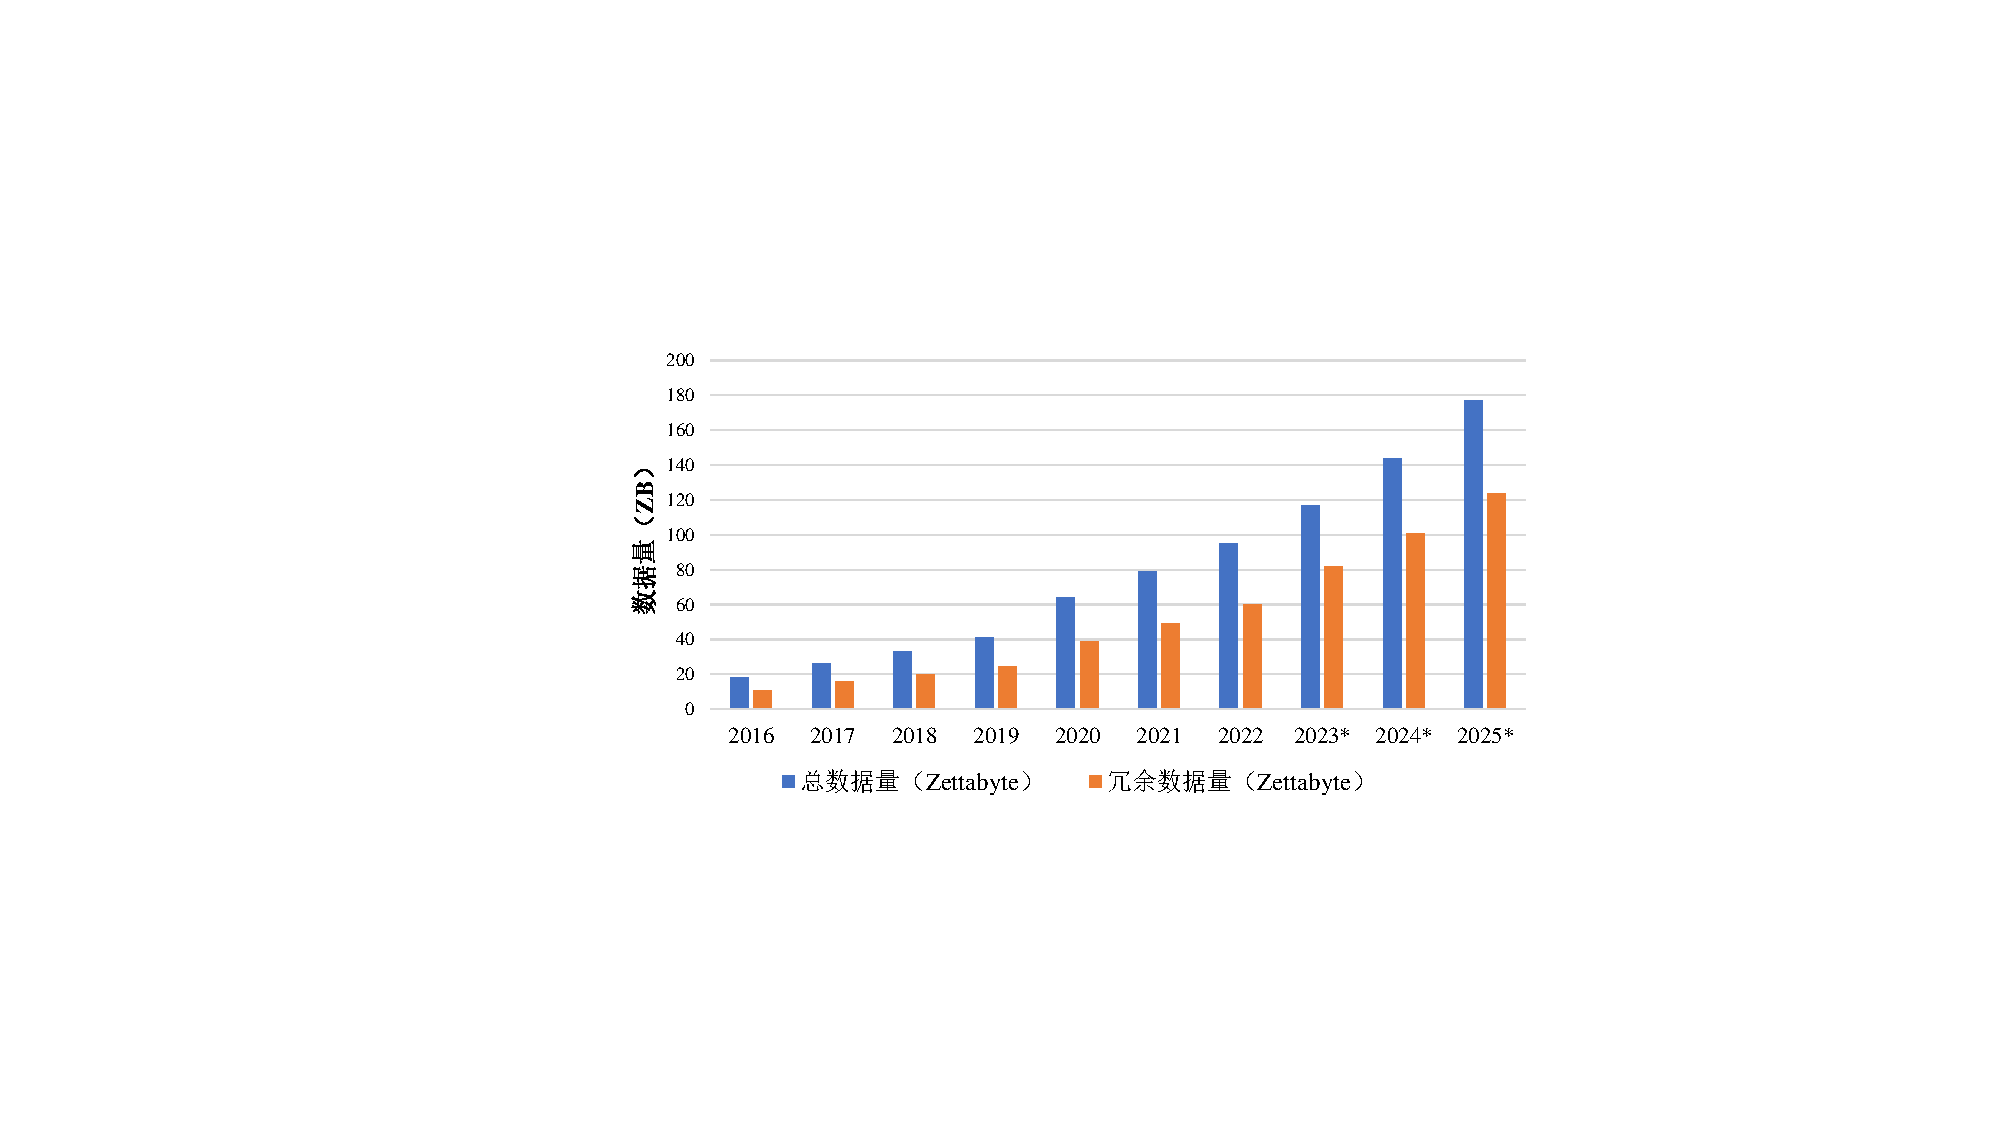
\includegraphics[width = 0.9\linewidth]{pic/数据增长图}
    \caption{数据总量和冗余量的增长及预测}
    \label{数据总量和冗余量的增长及预测}
\end{figure}

数据的爆炸式增长不仅要求研究人员致力于节约存储容量的研究,还要求人们投入更多的精力关注敏感数据的安全存储当中。根据\acrlong{ITRC}的数据显示\citing{databreach}:与2021年同期相比,2022年第一季度实际报告的数据泄露事件数量大幅度上涨,达到惊人的404起,增加了14\%。勒索软件攻击的平均支付额显著增加,远远超过往年的水平。下表\ref{2022年十大数据泄漏事件}
\citing{databreach}盘点2022年最大规模的十个数据泄漏事件涉及的公司及受影响人数。其中某几个公司的数据泄漏事件多次发生,波及人数千万计。可见,敏感数据的安全存储技术发展迫在眉睫。

\begin{table}[htbp]
    \begin{center}
        \caption{2022年十大数据泄漏事件}
        \label{2022年十大数据泄漏事件}
        \begin{tabular}{|c|c|}
            \hline
            \textbf{公司名称}             & \textbf{波及人数(万人)} \\
            \hline
            Cash App Investing            & 820                       \\
            \hline
            Beetle Eye                    & 700                       \\
            \hline
            FlexBooker                    & 375                       \\
            \hline
            Elephant Insurance Services   & 276                       \\
            \hline
            Lakeview Loan Servicing       & 257                       \\
            \hline
            Horizon Actuarial Services    & 229                       \\
            \hline
            Shields Health Care Group     & 200                       \\
            \hline
            Texas Department of Insurance & 180                       \\
            \hline
            Flagstar Bank                 & 154                       \\
            \hline
            Baptist Medical Center        & 124                       \\
            \hline
        \end{tabular}
    \end{center}
\end{table}

数据量指数级增长和敏感用户数据泄漏问题给存储系统研究人员带来了巨大的挑战和机遇,因此近年来关于安全和高性能的存储系统研究层出不穷。其中,以密文去重的存储系统最为有效,下文简述该系统的研究发展。


当前的数据存储系统主要都是以数据块为粒度进行存取的,所以研究密文去重技术往往也是从研究数据块存储技术开始。数据块存储是一种控制数据存储和存储设备的技术。它将任何对外存数据的操作转化为对数据块的操作,进而按照一定的规则进行恢复成逻辑文件内容或者切分成若干数据块存放在外存中。去重技术往往是按照数据块粒度开展的,所以叫块数据去重。基于块存储的去重技术是指存储系统中只会存储重复数据块的一份物理副本,而重复的数据块不会存放实际数据但会存放一个指向物理副本的引用。因为指针占用物理空间极小,所以这样的操作很节约存储开销。当下,无论主存储系统(主存储系统是指个人电脑、台式机的存储系统,叫primary storage system,数据冗余度较小)\citing{meyer2012study}还是备份存储系统(备份存储系统是指云服务器的存储系统,叫backup storage system,数据冗余度交大)\citing{zhu2008avoiding, lillibridgesparse, wallace2012characteristics}广泛使用块数据去重技术,用来实现高度的存储空间的节约。以往的研究表明:块数据的去重技术可以有效地将主存储系统的存储空间减少50$\%$左右\citing{meyer2012study},将备份存储系统的存储空间减少98$\%$\citing{wallace2012characteristics}左右。因此,为了降低存储成本,大量云服务商的备份系统都会充分使用块数据去重技术,例如Dropbox、AWS和Alibaba Cloud\citing{harnik2010side, paulo2014survey}等。不仅如此,一些现有的操作系统能支持主存储机器上的数据去重,例如EMC的VNX/VNX2和Netapp的FAS系列\citing{paulo2014survey}。

为了提供安全性的保证,密文去重技术提供了一个加密层\citing{bellare2013message, keelveedhi2013dupless},以确保数据信息在写入可去重数据存储系统之前被加密。这种加密可通过对称密钥加密的方式来实现,而密钥来自于数据块本身的内容,例如,密钥被设置为数据块内容本身的哈希值。
这样,重复的明文数据块在加密后也会是确定的且相同的密文数据块,因此也可经过去重处理,即可对加密的数据块应用数据去重技术,以达到节约存储空间的目的。ClearBox\citing{armknecht2015transparent}、DupLESS\citing{keelveedhi2013dupless}、CDStore\citing{li2015cdstore}和REED\citing{qin2017design}等诸多研究已经设计了各种加密数据去重方案。这些方案大致都能被概括为一个共性去重系统框架,见图\ref{加密数据重复与删除系统逻辑视图}。具体来讲,客户端首先选用固定大小或者可变大小的数据块切分算法将逻辑文件切分成大小相等或者不等的若干逻辑数据块;对每一个逻辑数据块进行加密算法计算形成密文数据块,并将这些密文数据块发送至服务端。服务端先用指纹函数(参考\ref{指纹})提取密文块的指纹值(fingerprint)对照指纹索引判断是否是唯一的(unique),如果是唯一的话,需要在指纹中加上新索引项。最后,服务端更新密钥元数据和文件元数据,以及将新数据块存放在外存。其中更新密钥元数据就是记录该密文数据块的加密密钥等信息,更新文件元数据就是记录组成逻辑文件的密文数据块的具体物理外存的位置等相关信息。

\begin{figure}[htbp]
    \centering
    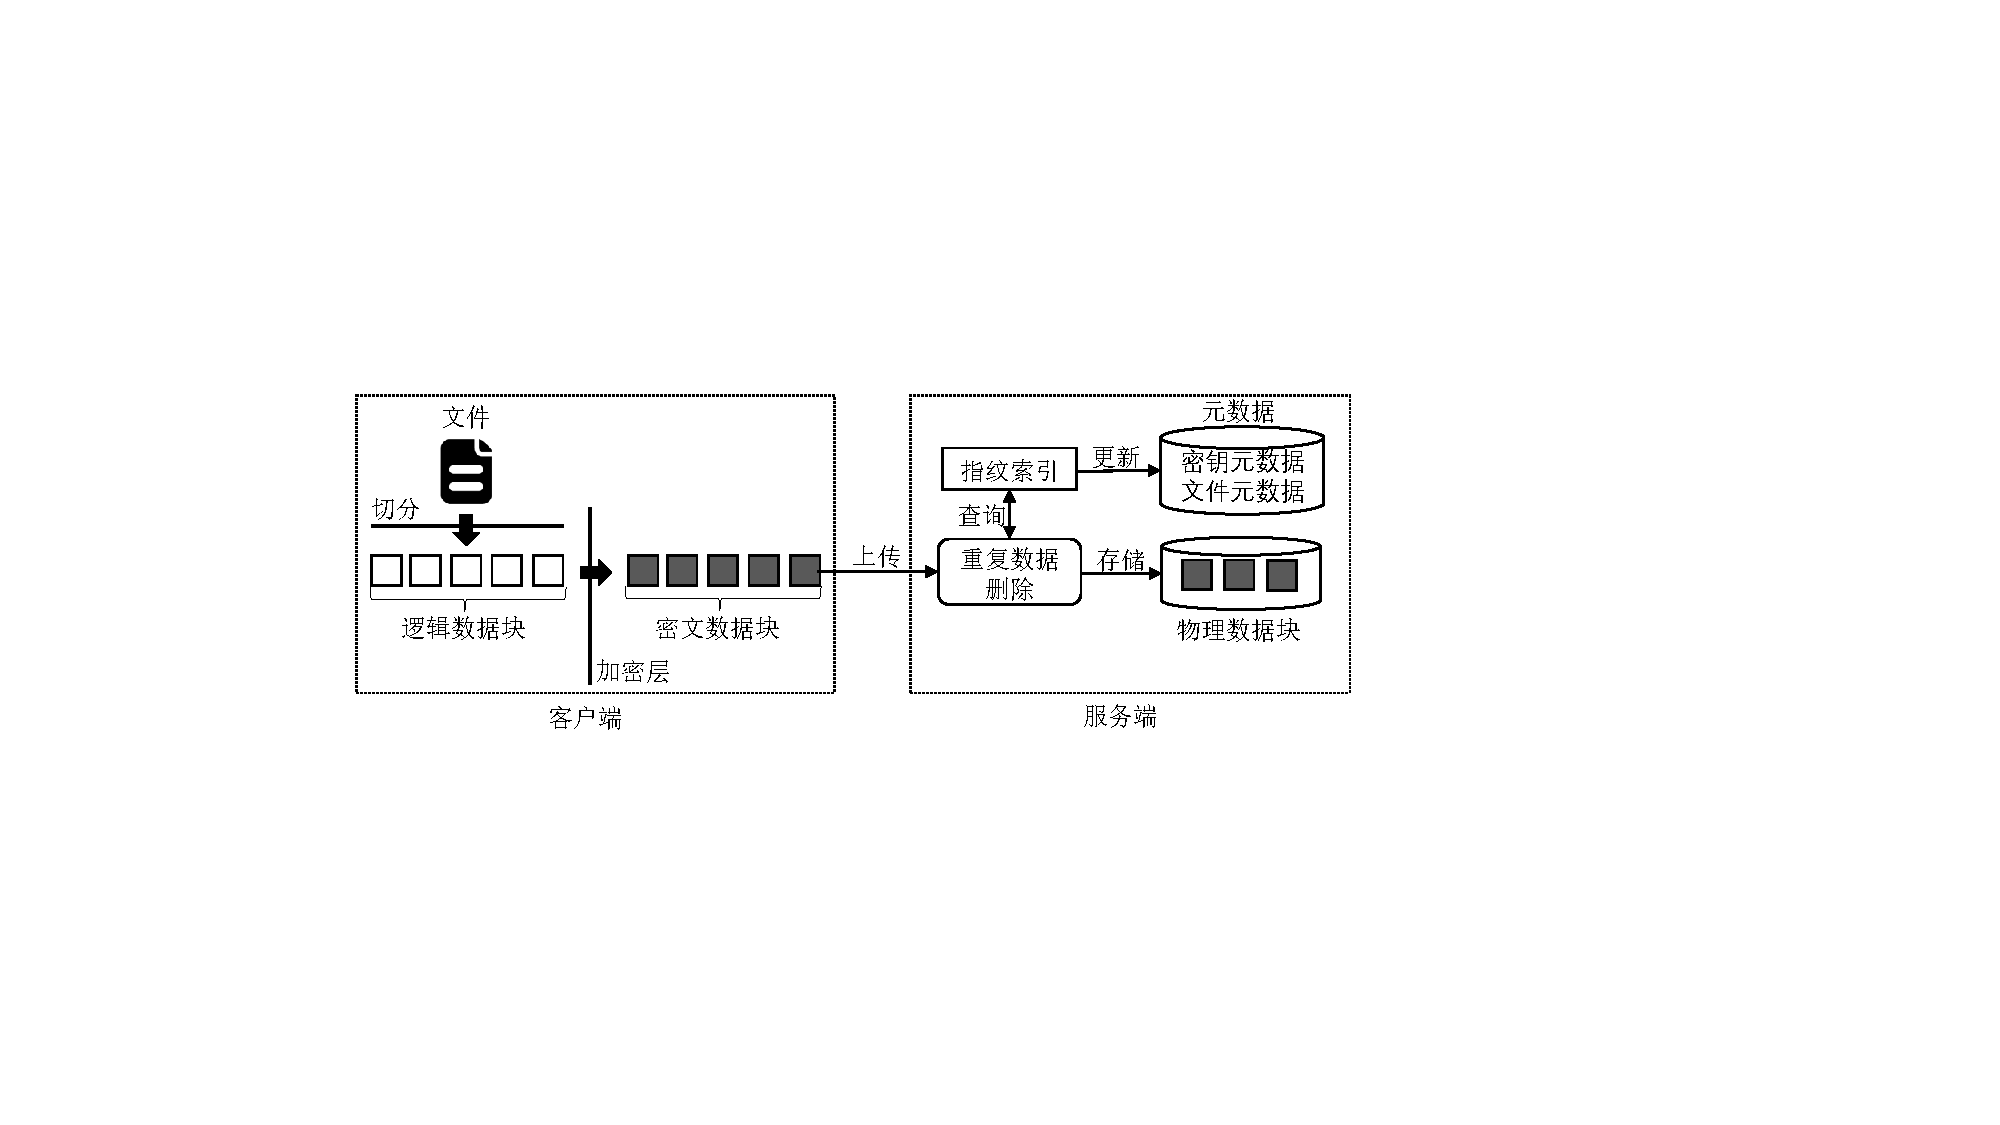
\includegraphics[width = 1.0\linewidth]{pic/加密数据重复与删除系统逻辑图}
    \caption{加密数据重复与删除系统逻辑视图}
    \label{加密数据重复与删除系统逻辑视图}
\end{figure}

除了考虑基础的密文安全性保障之外,应用数据去重技术的存储系统还需要考虑额外的功能,比如:兼容高效密钥更新和密文关键词检索的功能。密钥更新的功能是指用户在上传加密数据至云端之后,可以更新密钥并对已上传的文件重加密,该功能保证了数据去重系统的密钥安全性以及访问权限撤销的功能性\citing{qin2017design};密文关键词检索功能是指使用可搜索加密技术实现,在服务端不知道关键词明文的前提下对关键词关联的文件进行检索的功能,该功能极大地减小了传统方法所占用的网络带宽,比如用户端下载密文再解密检索,还能在一定程度上规避掉诚实且好奇的云服务端刺探隐私数据的风险\citing{song2000practical}。

兼容高效密钥更新的功能,众所周知,是一个至关重要的保障密文安全的手段。在多用户使用云存储服务的环境下,密文去重系统向各个用户开发密钥更新的接口,这样文件属主有选择地下载云端文件、更新加密、上传。同一份数据进行多次加密生成不同的密文,那么去重操作需要多次被应用在不同的密文上,反复计算会浪费宝贵的CPU资源,同时随之产生大量的网络I/O。本论文认为密钥更新带来的网络带宽占用和CPU资源的损失远超于去重带来的空间收益,因此提出一种新型的、既能兼顾存储效能又能减少因密钥更新带来的额外开销的密钥更新技术是十分有必要的\citing{qin2017design}。

密文去重系统中关键词检索、关联分析和密态推荐一直是一个研究的痛点。在遇到如何对密文进行检索的难题时,最简单的方法就是对文件下载解密再查询。这种方法往往不适用,它导致网络开销和计算开销的浪费,原因是下载了不必要的文件并且解密和查询的成本很高\citing{song2000practical}。云服务器的计算能力强大,因此人们希望能够利用其进行检索功能。然而,由于云服务器通常是“诚实且半可信”的,用户的隐私面临暴露出来,虽然可以把密钥发送给云服务器并由服务器进行解密和查询,但这种方法可能存在隐私泄露的风险。可搜索加密技术应运而生,但并没有前人的工作很好地将其和关联分析,密态推荐融合起来,也没有相关工作揭露一个具备完整的检索功能的密文去重系统样貌。


\section{国内外研究现状}
\subsection{密文去重技术删除研究进展}\label{ciphertext_dedup}
密文去重技术按照粒度可简单分为文件级数据去重和数据块数据去重,文件级粒度上的去重技术相对简单,目前相关研究工作较少;与文件级去重相比,数据块级的去重技术能够检测和删除更多的冗余信息(例如相似的文件中的相同数据块),但实现的复杂程度也相应增加。

早期的密文去重系统以基本\acrshort{MLE}(message-locked encryption)搭建\citing{anderson2010fast, cox2002pastiche, wilcox2008tahoe},易于受到暴力破解攻击。例如,频率分析攻击。频率分析是一种针对确定性加密的密码分析技术。假设攻击者已知某明文集合,致力于推测目标密文集合内各密文对应的原始明文(注:这里的集合均包含重复的明文或密文)。为了实施频率分析,攻击者根据出现频率分别对明文和密文进行排序,然后将每个密文映射为与其具有相同排名的明文。该技术已被应用于破解匿名日志\citing{kumar2007anonymizing}、破坏关键词隐私\citing{islam2012access}、重构密文数据库记录\citing{naveed2015inference}等实际攻击。
服务器辅助 \acrshort{MLE} 是当前密文去重系统所采用的主流方法\citing{keelveedhi2013dupless, shah2015lamassu, zheng2015enabling, armknecht2015transparent},DupLESS\citing{keelveedhi2013dupless}是其中的代表性系统。DupLESS 实现了一个专门的密钥服务器来管理系统密钥,该密钥服务器使用 RSA 盲签名方法来产生\acrshort{MLE}
密钥,并实施速率限制机制防止恶意用户的在线暴力攻击。Duan\citing{duan2014distributed}证明,在当前的重复数据消除模式下,使用除数据本身之外的其他秘密来生成加密密钥可以实现最佳的安全性。然后,Duan引入了一种分布式协议,该协议消除了对密钥服务器的需求,并允许较少管理的系统(如P2P系统)享受高安全级别。

当前的数据块级密文去重系统包括 Dekey\citing{li2013secure}、CDStore\citing{li2015cdstore}和 SecDep\citing{zhou2015secdep}。以下对这三个系统做简要分析。

Dekey系统里用户不需要自己管理任何密钥,而是在多个服务器上安全地分发收敛密钥共享。安全分析表明,Dekey在所提出的安全模型中指定的定义方面是安全的。Dekey使用Ramp密钥共享方案(RSSS)来实现,并证明在现实环境中的开销有限。

CDStore建立在一种称为收敛分散(convergent dispersal)的增强密钥共享方案的基础上,该方案通过使用确定性内容派生的散列值作为密钥共享的输入来支持s数据去重,CDStore的设计将收敛分散与两级数据去重消除相结合,以实现带宽和存储节省,并对侧信道攻击具有鲁棒性,CDStore比基准云存储解决方案节省了70\%的资金成本。

SecDep采用用户感知收敛加密(UACE)和多级密钥管理(MLK)方法:UACE结合了跨用户文件级和内部用户块级数据去重技术,并利用用户之间和内部的不同安全策略将计算开销降至最低。具体来说,文件级和块级s数据去重都使用收敛加密(CE)的变体来抵抗暴力攻击。主要区别在于,文件级收敛加密的密钥是使用服务器辅助方法生成的,以确保跨用户数据去重的安全性,而块级密钥是使用用户辅助方法生成,计算开销较低。为了减少密钥空间开销,多级密钥管理方法使用文件级密钥来加密块级密钥,以便密钥空间不会随着共享用户的数量而增加。此外,多级密钥管理方法将文件级密钥拆分为共享级密钥,并将它们分发到多个密钥服务器,以确保文件级密钥的安全性和可靠性。安全分析表明,SecDep确保了数据机密性和密钥安全性。基于几个大型真实世界数据集的实验结果表明,与最先进的数据去重方法相比,SecDep更具时间效率和密钥空间效率。

\subsection{密文关键词检索研究进展}\label{密文关键词检索技术研究进展}
当前,密文关键词检索功能主要是通过可搜索加密(SE,searchable encryption)技术来实现的\citing{song2000practical}
可搜索加密主要包含对称可搜索加密(SSE,symmetric searchable encryption)和非对称可搜索加密(ASE,asymmetric searchable encryption)2种类型,这2种类型来源于不同的现实问题,用来解决不同的需求问题。对称可搜索加密解决的是不可信的云服务端存储问题,举例来说,当用户Alice将数据加密存储在云服务端并需要检索某个关键词是否被数据包含时,无需将整个数据下载、解密和检索明文关键词的浪费计算资源和网络带宽的操作,引入一种新型加密方法:对加密后的文件可以执行检索功能,并在这个过程中不会泄漏任何明文的敏感信息。非对称可搜索加密解决的是不可信赖服务器路由问题,举例来说,用户Bob通过一个不信赖的邮件服务器向用户Alice发送邮件,该邮件服务器在不能获取邮件内容和敏感关键词信息的前提下会根据邮件包含的不同关键词发送到不同的终端。


由于本论文的系统属于典型的不可信赖的云服务端存储系统,所以本章节后续部分只针对对称可搜索加密算法做综述。
Song等人\citing{song2000practical}在对称密码体制下引入可搜索加密,提出了SSE(symmetric searchable encryption)概念,同时也提出了首个对称可搜索加密的构造方案包括SWP方案\citing{song2000practical}。SWP方案将文件切分为长度固定的单词,并采用分组加密和流密码加密相结合的方法,使得服务器不能获取任何明文相关信息,但是因需要全文扫描而算法效率极其低下,并且该算法极其容易受到统计攻击的威胁。由于Song等人\citing{song2000practical}在提出SWP构造方案时,并没有进行安全性定义,Curtmola等人\citing{curtmola2006searchable}在2006年提出了安全性的定义,与此同时提出了两种SSE方案,即SSE-1和SSE-2。其中,SSE-1是非适应性安全的构造方法,但检索效率高:数组存储着关键词加密结果,速查表(一个倒排索引)存放着关键词信息和其在数组中的位置;SSE-2是适应性安全的构造方法,但是需要占用更大的通讯带宽和服务器存储资源:不像SSE-1中维持链表,而是对每一个关键词建立关键词族,并建立关键词组成员到文件的映射关系。

除了以上经典的构造方案以外,2010年来有很多适用于不同场景的新式方案被提出。Wang等人\citing{wang2010secure}定义了加密云数据上的安全排序关键字搜索问题,并提供了这样一种有效的协议,该协议实现了安全的排序对称可搜索加密的定义,几乎没有关键字关联的隐私信息泄漏。Premasathian等人\citing{premasathian2012searchable}提出了一种不需要计算陷门值(trapdoor)的密文检索方案:用中国剩余理论(Chinese Reminder Theorem,CRT)判断两个密文检索算法得到的同余方程组的最小正整数是否存在来判断密文中是否含有某一个关键词。Cash等人\citing{cash2013highly}提出了一个可搜索对称加密(SSE)协议的设计和分析,该协议支持对外包对称加密数据的联合搜索和一般布尔查询,并可扩展到非常大的数据库和任意结构的数据。对于联合搜索的情况,以前的SSE构造要求数据库中文档总数的线性工作,并且仅为结构化属性值数据提供良好的隐私,这使得这些解决方案对于大型实用数据库来说过于缓慢和不灵活。相比之下,Cash等人的解决方案通过有效地支持非常大的数据库,在性能和隐私之间提供了一种现实和实用的权衡,代价是向外源服务器的适度和明确的泄漏(泄漏是以数据访问模式的形式出现的,而不是直接暴露明文数据或搜索值)。Cash等人还对协议的隐私和安全性进行了详细的形式密码分析,并建立了允许泄漏的精确上限。Cao等人\citing{cao2013privacy}首次定义和解决隐私保护的多关键词排名搜索问题(Multi-keyword Ranked Search, MRSE):选择关键词的“坐标匹配”,尽可能多的匹配关键词和文档关联性,换句话说就是采用文档中出现的关键词数量,定量评估文档与搜索信息的关联度。Dai等人\citing{dai2019privacy}于2019年提出了混合云上的多关键词排名搜索问题的解决方案:将现有机器学习算法去计算并预测多个关键词之间的关联度,并以此为基础建立混合元多关键词检索的框架。

%将相关知识背景中存在的问题和该段放在一起 单拿出来形成一章节:现有系统不足以及研究动机
\section{现有系统的不足及研究动机}\label{现有系统的不足和研究动机}
正如\ref{ciphertext_dedup}所展示,现有的密文去重系统虽然解决了一些分布式安全存储系统的中问题,但仍没考虑到问题有三点:

(1)用户为了更高的安全性会选择去更新文件密钥和撤销指定用户的权限。MLE密钥机制(参考\ref{消息锁加密})在密文去重的应用中,保证了相同的明文不会生成不同的密文,但同时也带来了文件重加密,即密钥更新的问题。存在一个这样的场景:现有一份相同的文件被多个用户拥有,他们均采用DupLESS机制\citing{keelveedhi2013dupless}获取相同的文件密钥,所以一份相同的密文在云服务上被共享。当他们其中任意一个用户的文件密钥可能被泄漏时(例如,存储文件解密密钥的设备被非法访问),那么该用户需要对文件重新加密。

针对文件重新加密,即密钥更新的问题,以下两种简单的方式常常被使用:\ding{172}一个对称密钥被用户重新生成,用户使用这个密钥对文件进行重新加密。用户首先从云服务器上下载原始密文,并采用原始密钥解密,之后用新的文件密钥对文件重新加密,并将新密文上传至云服务器。\ding{173}密钥服务器更换签名密钥。当一个用户需要进行重加密时,便请求密钥服务器更新签名密钥,即用户重新将文件的哈希值盲化,通过与密钥服务器交互获取一个新的文件密钥。用户采用新密钥将文件重加密之后,将新密文上传至服务器。

虽然以上两种方法实现过程相对简单,但是也存在很多缺点:数据去重效能不高,新上传的密文和旧密文不相同且独立,难以实现去重,所以相同的明文会在服务器存放多个密文的副本,严重浪费存储资源;不能保护用户数据机密性,即旧的密文任然存在于云服务器中,拥有某一个历史密文数据版本的密钥依旧可以获取明文信息;通信开销大,需要将整个新密文上传至云服务器,占用了极大的网络带宽和计算资源。

(2)密文关键词检索时往往不具备关联分析与推荐的功能。以往的工作很少能考虑到百万级数据的密文检索效率瓶颈问题,即包含同一个密文关键词的文件在分布式系统中有成千上万个。即使建立了密文关键词和文件名的倒排索引,数以万计的文件数量在被执行检索时也会占用极大的CPU资源和内存空间。此外,将如此数量的文件全部传输给用户,供用户去筛选和抉择自己想要的文件不仅占用了很大的网络带宽,还给用户带来了极差的体验。所以,在密文检索的功能设计中,往往要考虑关联分析和推荐的功能。也就是说,云服务能够智能化地对密文关键词和关键词、关键词和文件之间关联进行分析并将用户最有可能想要检索的若干文件或关键词筛选出来推荐给用户。

(3)当前的密文去重系统不具备边缘服务器和云服务器架构的适配性。边缘计算是指使用用户或者数据源附近的物理机进行计算,这样能降低延迟和节约带宽,所以近年来非常受关注\citing{yu2017survey}。此外,边缘计算和中心云计算机并行计算的方式加速数据计算速度和提高数据备份的容灾性\citing{cao2020overview}。然而,当前无论是密文关键词检索功能还是密文去重系统都不具备“云边协同”服务架构的适配性。也就是说,当前的密文检索功能或密文去重系统都是用在中心化的云服务器上的,在云服务器和边缘服务器的架构上还不能很好地被应用。其中,密文检索功能在“云边协同”架构上应用需要考虑的是在安全和低延迟的前提下对多个边缘服务器下的密文关键词和文件进行关联性分析;密文去重系统在“云边协同”上的架构需要考虑整体系统的安全性、功能性以及存储效能。

总结来说,目前没有一个具备密文关键词检索和推荐功能、用户可选择更新文件密钥功能的适用于云边协同架构的分布式密文去重系统。

\section{本文的主要贡献和创新点}\label{本文的主要贡献和创新点}
为了设计一个具备密文关键词检索和推荐功能、用户可选择性更新文件密钥功能的适用于云边协同架构的密文去重系统,本论文设计了一套基于云边协同架构功能完整的密文去重系统。本文论文的贡献总结如下:

(1)基于CANOT安全高效的兼容密钥高效更新的加密技术。CAONT是一种无需密钥随机变换模式,可将原始明文转换成CAONT密文(称为CAONT package),保证了攻击者即使获取了部分CAONT package,也无法恢复原始明文。CAONT package由存根(stub)和修剪包(trimmed package)两个部分组成,将CAONT内部的随机因子替换成明文的hash值,这样相同的明文就可以被加密成相同的密文,从而支持数据去重。其中的存根部分可以由文件主选择的文件密钥加密,因为其占比小,当文件密钥更新时,所占用的网络资源和计算机相应地减小很多。本论文的密文去重系统,利用基于CAONT的加密技术达到了高效密钥更新和支持懒惰更新的动态访问控制的功能。

(2)设计简约但性能优越的密文检索算法,并增加密态关联和推荐的功能。现有的可搜索加密技术无论基于哪种思想,要么需要全文关键词检索,要么需要对索引进行全表扫描,存在一定的性能瓶颈,需要巧妙的设计增强检索性能,尤其是关键词不命中的检索性能;现有的密文检索功能只能做到检索和关键词关联的文件信息,但是并没有良好的关联分析和推荐功能,用户体验较差。本论文的密文去重系统将基础密文推荐技术进行改造,加入密文关键词的图关联信息,根据图中边权可推荐关联性最高的若干关键词和关联文件,因此具备了良好的密文检索和推荐功能。

(3)云服务器和边缘服务器协同架构上的两级去重方案。本论文以一个中心化的云服务器和多个边缘服务器的协同的,类似于“花蕊和花瓣”的架构模式。其中,每一个边缘服务器在不同的机构里部署,并且只为该机构下的所有用户服务,本论文在边缘服务器上进行文件级粒度的去重,这样保证了来源于同一个文件的数据块往往存储位置相邻,大大加快数据的读写速度;中心化的云服务器是为每一个边缘服务器提供服务的,本论文在云服务上对来源于不同边缘服务器的数据块进行细粒度的去重,在作为各边缘服务器的存储备份的同时,能进一步节约存储开销。此外,中心化的云服务还能对来源于不同边缘服务下的关键词进行关联分析,达到跨服务的推荐效果。

(4)最后,本论文将基于AONT安全高效的兼容密钥更新的技术增强的基础密文推荐的技术融于云边两级去重架构上,完成了一个具备完备功能的密文去重系统。本论文用合成数据集和真实数据集两种环境进行模拟实验,不仅测试了该原型系统的密文去重、密钥更新和密文检索与推荐的各个模块子功能,还对存储效能、密钥更新效率和数据上传下载速度多方面进行性能测试。实验结果表明,各模块子功能完善,各个方面性能相对优越,可以算得上是一个优良的完备密文去重原型系统。


\section{本文的结构安排}
本论文共计五个章节,章节结构安排如下:

第一章作为绪论部分,简明扼要地介绍了去重技术,并交代了具备加密层的去重技术,即密文去重技术,继而进一步提出了密文去重系统中往往需要考虑的两个方面的问题,包括了为了更高的安全性密钥更新的问题和密文关键词检索的问题。然后,根据这两个方面从国内外的研究现状分析密文去重系统的方案和不足。最后,提出了本论文的去重系统与现有系统相比而言功能完备性和研究的创新性。

第二章首先讲述了密文去重系统涉及的若干要点:去重的流程和分类,关键数据结构和重要概念。然后,对可搜索加密做了简要阐述。其次,对现有关联分析和密文推荐技术做了综述,着力于分析现有技术的挑战。最后,分析云边协同的概念、应用和涉及的安全问题。

第三章节主要针对密文去重系统的两部分技术核心做了详细交代。首先交代了系统架构,介绍系统整体外观并交代了这种架构方式的优势。然后,分析威胁模型并引入本系统设计的三个安全性目标。为了达成这三个安全性目标,本论文有条理地介绍了两大核心技术点:兼容密钥更新的安全高效的密文去重技术和兼具关联性推荐的密文检索技术。在密文去重技术中,详细交代了安全和高效的突出点以及是如何兼容密钥更新的;在密文检索技术中,详细阐述关联值的公式表述和更新以及关联分析和推荐的功能实现流程。最后,在每个技术点后面都交代了对“云边协同”架构适配性,并且在密文检索技术的最后交代了两个技术点的兼容性。

第四章节主要对系统实现和实验做详细说明。本章主要分为两个部分,第一部分详细地介绍了整个系统各个组成的底层实现和优化,其中至关重要的是作为和用户的交互接口,即客户端的实现;边缘服务器的实现在于直接为客户端提供服务;云服务器的实现核心在于对庞大的数据块索引进行压缩索引方式的优化加快了索引访问速度;第二部分主要是整个实验环节:先交代了实验的实施方案,然后从各个方面展示实验的结果以及本系统的性能优势。

\section{本章小结}
本章作为绪论,粗浅简单地介绍了明文和密文去重技术、可搜索加密技术的发展,最后提出了本文的密文去重系统关注的两个方面问题:密钥更新问题和密文检索检索问题。以此综合国内外发展现状分析现有系统的不足以及本论文的动机。继而,对现有密文去重系统进行批判性总结并简要地说明本论文密文去重系统的优势,即本论文的贡献点。最后,简单交代了本论文的章节安排。

\chapter{相关知识背景}

\section{密文去重系统}

\subsection{数据去重技术}\label{指纹}
数据去重技术是一种可以节约存储空间的数据存储技术\citing{xia2016comprehensive},同时又被称为重复数据删除技术。数据去重技术按照粒度被分为文件级去重技术(粒度大)和数据块级去重技术(粒度小)。其中,文件级去重技术的核心思想是:对文件整体内容做哈希运算提取其指纹信息并存储在文件级指纹索引中,重复的指纹说明相同文件内容已经被存储过。文件级数据去重的去重率往往不高,因为两个相似的文件即使一个字符的差距也会生成不一样的文件级指纹,所以需要更细粒度的数据去重技术,即数据块级去重。

数据块级去重的核心思想是:将大量的数据划分为若干数据块(数据块的大小是固定的或者可变的),并计算每一个数据块的哈希值,称为数据块的“指纹”(fingerprint),以此来识别每一个数据块是否是唯一(unique)的或是否已经存储过(duplicate)。具体来说,利用哈希函数的防碰撞性使得不同的数据块具备唯一性的标识。将文件切分为若干大小相等或者大小可变的数据块之后,只需将这些数据块的内容转变为对应的数据流,传递给散列计算函数,那么可获得数据块对应的指纹(fingerprint)。用唯一性的指纹去标识每一个数据块,数据去重技术便可根据指纹标识来确定某新数据块是否存储过。若该新数据块是之前未被存储过的(unique),那么执行磁盘写操作存储该数据块;若该数据块是之前已经存储过的(duplicate),那么找到相同数据块的物理位置,建立指向该物理块的指针可用于恢复。这种方法往往也可以用在密文去重技术中,但是需要在加密模块中进行巧妙的设计才能兼容现有的明文数据去重技术。

数据去重技术从去重发生时机上又可以划分为在线去重(in-line deduplication)和离线去重(post-line deduplication)。在线数据去重意思是在数据写入磁盘或存储端的前进行数据分块、数据块指纹运算以及数据块指纹检索并判断是否需要真正落盘操作的流程。比如,大名鼎鼎的ZFS文件系统(Zettabyte File System)采用的就是在线去重方式。而离线数据去重是指先将数据一股脑全部写入到磁盘或者存储端,当系统空闲时,由后台线程读出数据块并进行指纹计算和数据块查重。在线去重和离线去重对比起来各有优劣,简单来说,在线去重牺牲了存储性能但收获了存储空间,而离线去重会先损失存储空间但是给用户良好的存储体验,当存储空间不足时离线存储功能是极为受限的。在此多赘述一句:本论文的系统采用的是在线去重的方式。

在数据去重系统中往往涉及两个重要的数据结构:指纹索引表(fingerprint index)和文件指纹序列(file recipe)。其中,指纹索引表维护在存储端,是全局唯一的,用于记录已经存放在磁盘上的数据块指纹值;文件指纹序列是指逻辑文件被切分成的逻辑数据块的指纹序列,用于恢复整个文件。指纹索引表和文件指纹序列又被统称为元数据(metadata)。

最后,简单阐述一下数据去重技术和数据压缩技术的区别:虽然两者目的都是减小数据的冗余,但压缩技术是采用压缩算法(例如,LZ77、Human等)深入编码层\citing{kodituwakku2010comparison},用尽量少的数码代表尽量多的信息,往往被用在信号传递和信息传输上,而数据去重技术是在数据块或文件粒度上减小数据存储空间。

\subsection{消息锁加密}\label{消息锁加密}%密文去重系统
在密文去重技术中,往往会遇到一个棘手的问题:数据块加密和数据去重的存储效能兼顾困难。比较直接点的方法是通过常用的加密算法,对称加密算法(比如,AES、DES等)或者非对称加密算法(比如,RSA)对数据块明文进行预处理,加密密钥由用户提供。

然而,由于不同的用户可能会选择不同的密钥对数据块进行加密,那么即使相同的明文块也会被加密成不同的密文块,去重后的存储效率大幅降低,所以这种直接的简单加密方法极其不利于数据去重技术的运用。详细来说,假设某一个的数据块$C$,被多个用户共享,用户Alice选择的加密密钥是$k$,那么该数据块经过加密后变成$[C]_k$;用户Bob选择的加密密钥是$k'$,那么该数据块进过加密之后结果是$[C]_{k'}$,此时$[C]_k \neq [C]_{k'}$。很明显,跨用户的密文去重技术几乎不可实现。更糟糕的是,即使单个用户使用不同的密钥对不同文件进行加密,来源于同一用户的相同数据也可能无法进行密文去重。此外,将非对称加密算法运用在加密层做如此简单的操作也会导致相同的问题,并且非对称加密算法性能开销更大而不能被良好地运用在密文去重系统中。

因此为了保证相同的明文块能被加密生成相同的密文块,Bellare等人\citing{bellare2013message, keelveedhi2013dupless}提出了消息锁加密(message-locked encryption,MLE)技术,它使用数据块内容本身生成对称加密密钥来加密数据块本身。该对称密钥被称为MLE密钥,例如,使用收敛加密算法\citing{douceur2002reclaiming}计算数据块内容的哈希值作为MLE密钥。如此即可确保数据块的明文和密文具备一一对应关系,即相同的明文数据块一定生成相同的密文数据块,此时便可将传统的明文数据去重技术运用到密文系统中。

MLE算法主要分类如下:

(1)早期MLE算法

早期MLE算法\citing{bellare2013message}(Historical MLE)是用基于文件数据本身内容上的某一些公开函数生成MLE密钥的。这样的密钥生成函数有加密哈希函数或者内容提取函数等,为不可预测的数据提供的最高安全性是语义安全性,同时,MLE潜在的缺点是密文相等性泄漏了潜在的明文相等性。当一个数据块从有限的集合中抽取出来时,那么容易受到离线暴力破解攻击\citing{bellare2013message}。具体来说,对于给定某个目标加密数据块,攻击者可以从有限的可能明文数据块中依次抽取并采用相同MLE加密方式进行加密,再和给定目标密文数据块进行比对,然后建议明文数据块和密文数据块的对应映射关系,完成离线暴力破解攻击。经典的收敛加密方案\citing{douceur2002reclaiming}就存在这样的内在缺陷。

(2)基于服务器辅助MLE算法\label{RSA盲签名}

为了抵御离线暴力字典攻击,DupLESS系统\citing{keelveedhi2013dupless}引入一个密钥服务器,该服务器采用盲签名的机制,协助用户基于文件哈希值信息生成文件加密密钥。用户通过与密钥服务器进行在线交互才能获取文件加密密钥,因此,用户将不能进行离线暴力字典攻击。此外,密钥服务器执行严格的用户请求签名速率,因而能够有效抵抗攻击者的在线暴力字典攻击。不妨假设密钥管理器的公钥$pk = \{N, e\}$,私钥$sk=\{d\}$,那么密钥服务器进行在线交互获取文件加密密钥的流程如下:

\ding{172}客户端向密钥管理服务器申请用户身份验证,验证通过则继续执行后续操作。

\ding{173}用户计算文件$f$的哈希值$H(f)$。

\ding{174}用户从正整数中选取随机数$r$,并利用随机数$r$将文件的哈希值盲化,并将盲化后的结果发送给密钥服务器,盲化公式如下:
\begin{equation}
    h^* = H(f) \cdot r^e\, mod\, N
\end{equation}

\ding{175}密钥服务器用私钥$sk = \{d\}$对$h^*$进行签名,并将签名后结果返回给客户端,公式如下:
\begin{equation}
    sig^* = (h^*)^d\,mod\,N
\end{equation}

\ding{176}客户端用第\ding{174}中的随机数$r$对来自于密钥服务器的签名去盲化操作,公式如下:
\begin{equation}
    sig = sig^* \cdot r^{-1}\,mod\,N
\end{equation}

\ding{177}客户端对去盲化后的签名值进行校验,验证公式如下:
\begin{equation}
    H(f) = sig^e
\end{equation}

\ding{178} 如果校验通过,客户端用$H(sig)$作为加密密钥。

本论文的数据块MLE密钥生成过程借鉴RSA盲签名的密钥管理服务器的思路,所以为了论文叙述的完整性,在此处详细叙述了RSA盲签名生成加密密钥的流程。

\section{可搜索加密}
在现代信息技术快速发展的背景下,随着云计算和大数据技术的不断发展,越来越多的数据被存储在云服务器上。但是,由于数据隐私和安全问题的存在,很多用户对于将自己的数据存储在云服务器上并进行关键词搜索还存在担忧。因此,如何在保护数据隐私的同时实现高效的关键词搜索成为了云计算和大数据领域亟待解决的问题。

可搜索加密技术是一种新型密码学方法,旨在解决数据隐私保护和检索效率问题。它允许在数据加密的同时,在密文领域进行关键词搜索。数据拥有者使用加密密钥对数据进行加密,并将密文上传到云服务器。然后,授权的数据使用者使用对称密钥生成陷门,发送到云服务器进行查询检索。云服务器检索每个上传文件的索引表,匹配陷门关键词并返回密文文件。最终,数据使用者使用解密密钥解密云服务器返回的密文文件\citing{song2000practical}。

在可搜索加密技术中,关键的问题是如何实现高效的关键词检索。为此,需要考虑索引的数据结构以及检索索引的算法,同时还需要在索引的建立过程中考虑到关联分析。索引数据结构可以选择树型结构、哈希表等多种方式,不同的数据结构有着不同的优劣,需要根据具体情况进行选择。检索算法方面,有传统的倒排索引、布隆过滤器、哈希索引等多种算法可以选择,其中倒排索引是应用最广泛的算法之一。在倒排索引中,首先将所有文档中出现的关键词提取出来,并建立一个以关键词为索引的倒排表,每个关键词对应着一个文档列表,列表中包含了包含该关键词的所有文档。在搜索时,只需根据用户输入的关键词从倒排表中找到对应的文档列表,即可快速定位到含有该关键词的文档\citing{bosch2014survey}。

另外,关联分析也是建立索引时需要考虑的因素之一。在搜索时,除了根据单个关键词进行检索外,还可以根据多个关键词之间的关联关系进行检索。例如,在搜索“计算机”这个关键词时,还可以同时搜索与“计算机”相关的关键词,如“编程”、“算法”等,从而得到更准确的搜索结果。

总之,实现高效的关键词检索需要综合考虑索引的数据结构、检索算法以及关联分析等多个因素,根据具体情况进行选择和优化,以提高搜索效率和准确性。

\section{关联分析}
关联分析是一种发现数据集中项之间关系的技术。它基于频繁项集的概念,频繁项集是指在一个数据集中经常同时出现的项的集合。通过计算频繁项集,我们可以找到项之间的关联规则,这些规则可以告诉我们,当某些项出现时,其他项也可能同时出现。
关联分析的应用非常广泛,包括市场营销、推荐系统、医学研究等领域。在市场营销中,关联分析可以帮助企业识别客户购买的商品之间的关联关系,从而进行更有效的推销活动。在推荐系统中,关联分析可以根据用户的历史购买记录和浏览行为,向用户推荐相关的商品。在医学研究中,关联分析可以帮助研究人员发现疾病和基因之间的关联关系,从而更好地理解疾病的发生机制。

关联分析的主要算法包括Apriori算法\citing{hegland2007apriori}和FP-Growth算法\citing{borgelt2005implementation}。Apriori算法是一种基于频繁项集的算法,它通过迭代的方式生成候选项集,并计算每个候选项集的支持度,从而找到频繁项集。FP-Growth算法是一种基于树形结构的算法,它将数据集压缩成一颗FP-Tree,然后利用FP-Tree来发现频繁项集。相比于Apriori算法,FP-Growth算法更加高效,能够处理大规模数据集。

关联分析面临的主要挑战之一是维度灾难。随着数据集维度的增加,计算频繁项集的时间和空间复杂度呈指数级增长。为了解决这个问题,可以采用维度削减和分布式计算等方法。另一个挑战是数据的稀疏性。在某些数据集中,频繁项集可能非常少,这会导致关联分析算法难以发现有用的规则。

\section{密态推荐}
密态推荐技术是一种基于矩阵分解的推荐算法。矩阵分解是一种将一个大矩阵分解成多个小矩阵的技术,其中每个小矩阵都包含原始矩阵中的一部分数据。在推荐系统中,我们可以使用矩阵分解将用户-物品评分矩阵分解成两个低秩矩阵,一个矩阵表示用户的偏好,另一个矩阵表示物品的特征。

密态推荐技术的主要算法包括SVD、NMF、PCA等。其中,SVD是一种基于奇异值分解的算法,它可以将一个矩阵分解成多个小矩阵,从而提取出矩阵中的关键特征\citing{hoecker1996svd}。NMF是一种基于非负矩阵分解的算法,它可以将一个矩阵分解成多个非负矩阵,从而发现矩阵中的潜在模式\citing{luo2014efficient}。PCA是一种基于主成分分析的算法,它可以将一个矩阵转化成多个主成分,从而提取出矩阵中的重要信息\citing{vozalis2007recommender}。

以机器学习为代表的密态推荐技术存在着诸多挑战,比如:过拟合问题、冷启动问题、数据稀疏问题和算法效率问题等。这也是本系统不采用以机器学习为代表的关联分析和密态推荐技术的本质原因。
\section{云边协同}
云边协同是指利用云计算和边缘计算相结合的技术,将数据处理和计算资源分布在云端和边缘设备上,以实现更高效、更快速的数据处理和应用程序部署。在云边协同技术中,云端负责大规模数据的存储和处理,边缘设备则负责实时数据采集和处理。云边协同技术将云端的高性能计算能力与边缘设备的低延迟、低能耗的特点相结合,可以极大地提高数据处理的效率,降低系统的响应时间,并减少数据传输带来的网络负载。

在传统的云计算架构中,所有数据都需要传输到云端进行处理,由于数据量大、传输时间长等原因,容易造成网络延迟和数据安全问题。而在云边协同架构中,一部分数据可以在边缘设备上进行处理,只有需要进行深度学习、机器学习等复杂计算时才将数据传输到云端,这样可以大大降低数据传输的量和网络延迟,提高数据处理效率。

云边协同技术在许多领域都有应用,例如智能家居、智能制造、智慧城市等。在智能家居领域,云边协同可以将传感器数据在边缘设备上进行实时处理,只有当需要进行语音识别、图像处理等复杂计算时才将数据传输到云端进行处理,这样可以大大提高智能家居设备的响应速度。在智能制造领域,云边协同可以将传感器数据在设备端进行实时监测和分析,只有当需要进行生产计划优化、故障诊断等复杂计算时才将数据传输到云端进行处理,这样可以提高生产效率和产品质量。在智慧城市领域,云边协同可以将传感器数据在边缘设备上进行实时分析和处理,只有当需要进行交通管理、安全监测等复杂计算时才将数据传输到云端进行处理,这样可以提高城市管理效率和居民生活质量。

在云边协同技术中,安全问题也是一个重要的考虑因素。由于边缘设备的安全性通常较差,攻击者可以通过攻击边缘设备来获取敏感数据或者入侵系统。因此,云边协同技术需要采取一系列的安全措施来保障数据的安全性和系统的稳定性。一种常见的安全措施是采用端到端的加密传输技术,对数据进行加密处理,只有授权用户才能解密数据,保护数据的机密性和完整性。另外,云边协同技术还可以通过访问控制、数据备份等方式来保障系统的可靠性和稳定性。

总的来说,云边协同技术是一种非常有前途的技术,在未来的智能化发展中具有重要的应用价值。随着边缘计算和物联网技术的不断发展,云边协同技术将在越来越多的领域得到应用,为人们的生产和生活带来更加便捷、高效、安全的体验。
\section{本章小结}
本章节首先用大量的篇幅讲述了密文去重系统涉及的若干要点:去重的流程和分类,关键数据结构和重要概念。然后,对可搜索加密做了简要阐述,为下文的密文关键词检索做好知识铺垫。其次,对现有关联分析和密文推荐技术做了综述,着力于分析现有技术的挑战,以此表明本论文的密文关键词检索的关联分析和推荐技术不落窠臼。最后,分析云边协同的概念、应用和涉及的安全问题,以此引出本论文的云边协同的架构中所要考虑的诸多重点。

\chapter{系统设计和技术细节}\label{系统设计和技术细节}
该章节将会对本论文密文去重系统涉及的几个技术点进行详细的介绍。其中,\ref{系统架构}章节简单介绍整个密文去重系统的系统架构,\ref{CAONT}章节会介绍基于CAONT(Convergent All-or-Nothing Transform)加密和高效密钥更新相关思想和技术,\ref{keyword_search}章节讲述本论文的密文关键词功能核心思想和兼容关联性推荐的亮点。

\section{系统架构}\label{系统架构}
本论文的密文去重系统采用C/S架构(客户端/服务器架构方式),不过服务端是“云边协同”的构架,即云服务器和边缘服务器协同的架构设计。“云边协同”要求我们有一个中心化、全局的服务器,即云服务器;有若干个边缘服务器,边缘服务器可视为不同机构独有的区域性服务器。如图\ref{密文两级去重系统架构图}所示,在用户端基于CAONT技术进行数据的分块和数据块加密,同时采取类似于DupLESS\citing{keelveedhi2013dupless}系统中可以提供给客户端访问MLE密钥的密钥管理器,这样每一个用户端可以咨询密钥管理器得到必要的加密密钥;边缘服务器作为每一个机构的区域性服务器,可以当做云服务的边缘缓存,顺序存储每一个物理文件,只进行文件级数据去重,而云服务器作为中心化服务进行全局的数据块级别的数据去重。

\begin{figure}[htbp] %画个大括号 
    \centering
    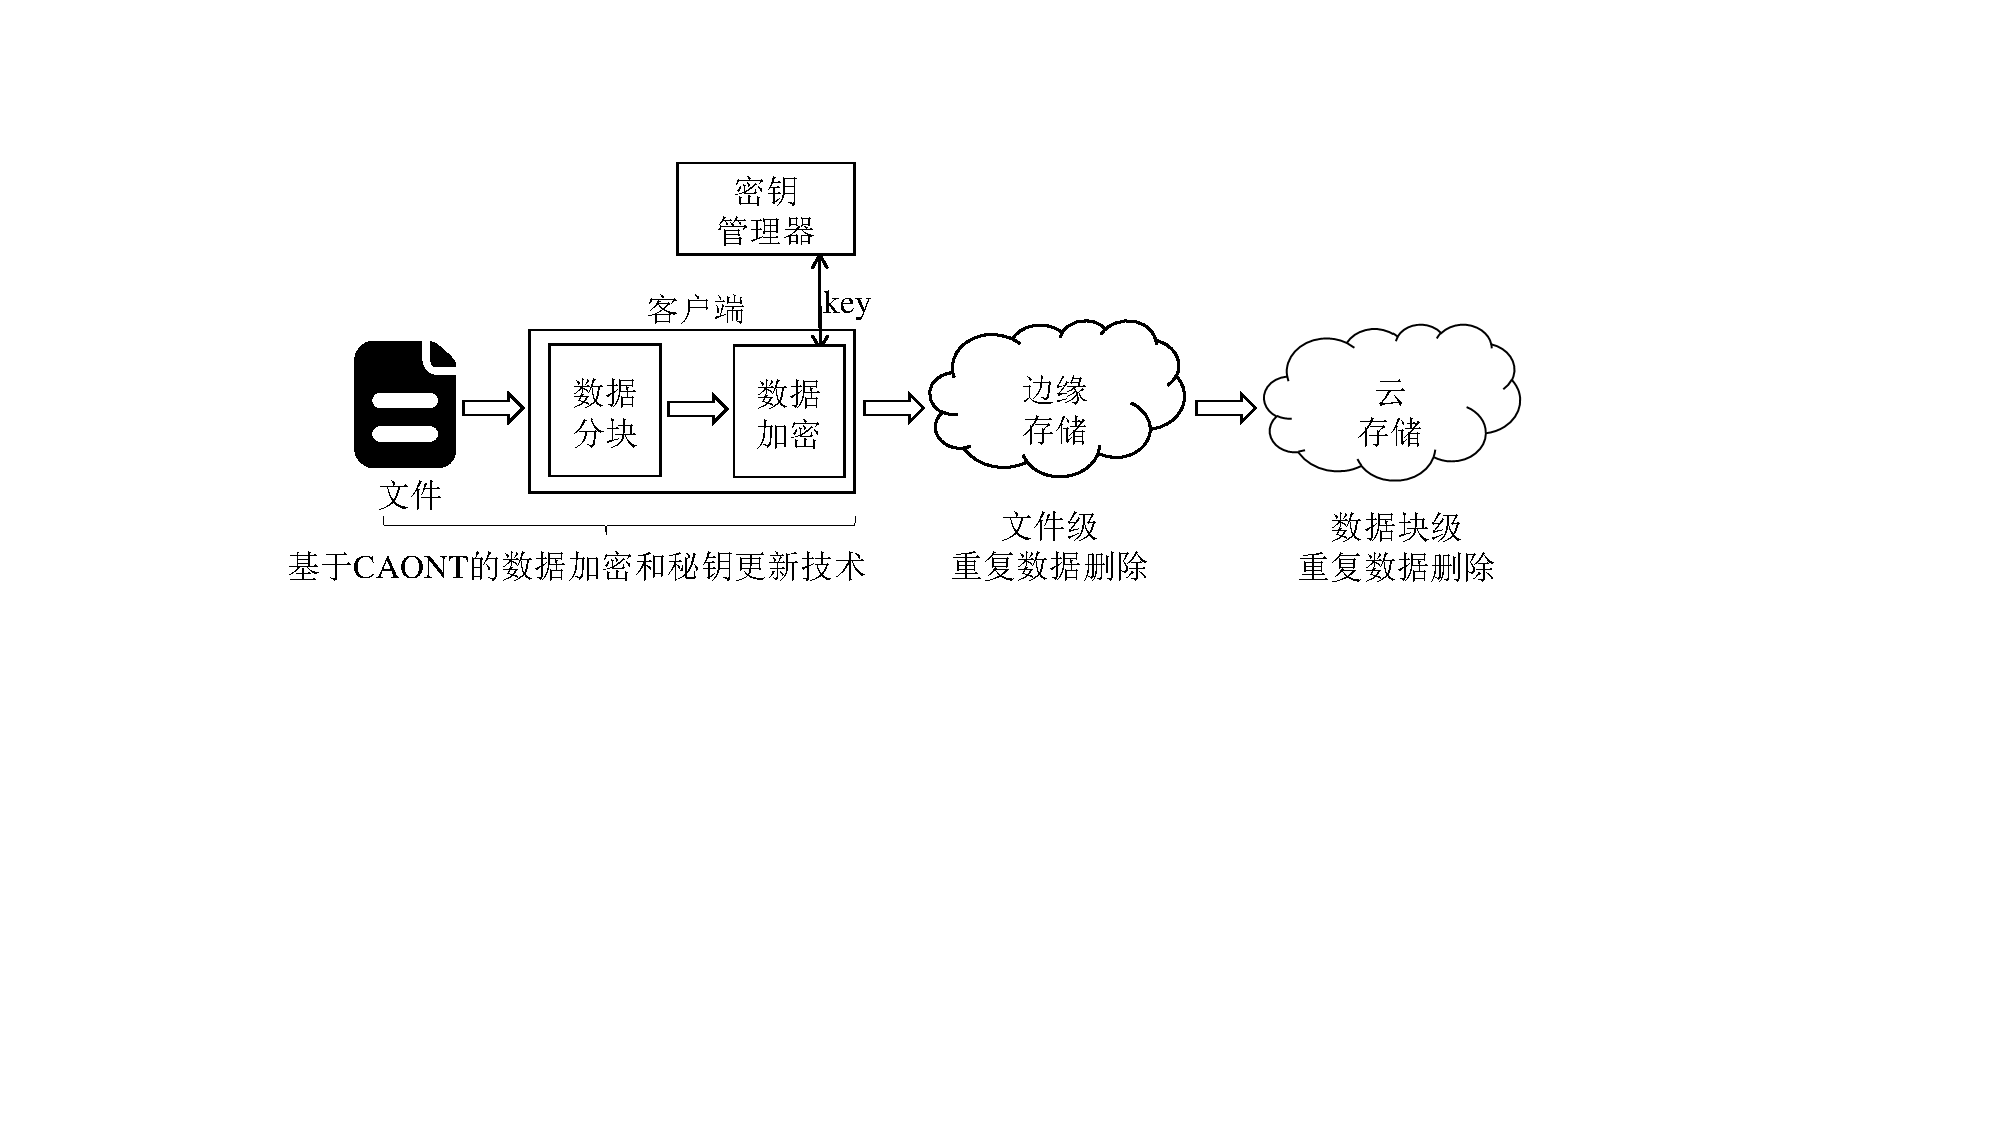
\includegraphics[width = 1.0\linewidth]{pic/jiagoutu.pdf}
    \caption{密文两级去重系统架构图}
    \label{密文两级去重系统架构图}
\end{figure}

在上传数据文件时,作为密文去重系统的入口,用户端会对要上传至服务端的数据本文进行分块(chunking),然后采用基于CAONT的数据加密技术对每一个数据块进行加密处理(加密密钥需要从密钥管理器获取,类似于DupLESS\citing{keelveedhi2013dupless}),得到密文数据块并上传至边缘服务器。边缘服务器会对整个密文数据整体做一个单向性的哈希运算得到总体密文的指纹值,即密文fingerprint。边缘服务器对密文进行文件级去重:维护一张边缘服务下全局性文件的指纹表,根据指纹表判断密文数据文件是否已被存放过,边缘服务器不对密文数据进行数据块级别的去重,仅仅将来自于同一文件的密文数据块顺序存放在边缘存储的外存上,最后上传密文数据块至云服务器上。云服务器会维护一张全局的数据块指纹索引表,并据此判断数据块是否已经被存储过,最后写入新的数据块。

在密文关键词检索时,用户端生成关键词门限(trapdoor)上传至边缘服务器,边缘服务器基于特定的数据结构进行检索和对比操作找到包含该关键词的关联度最大的若干文件以及关联度最大的其他若干关键词。此外,该边缘服务器会向云服务器请求其他边缘服务器的上密文检索结果,云服务收到该请求并转发请求,收集其他边缘服务的执行结果一并返回给该边缘服务器。最后,边缘服务器会将结果分类返回给客户端。图\ref{密文检索流程图}清楚地描述密文关键词的基本流程。

\begin{figure}[htbp]  %边缘存储和云存储
    \centering
    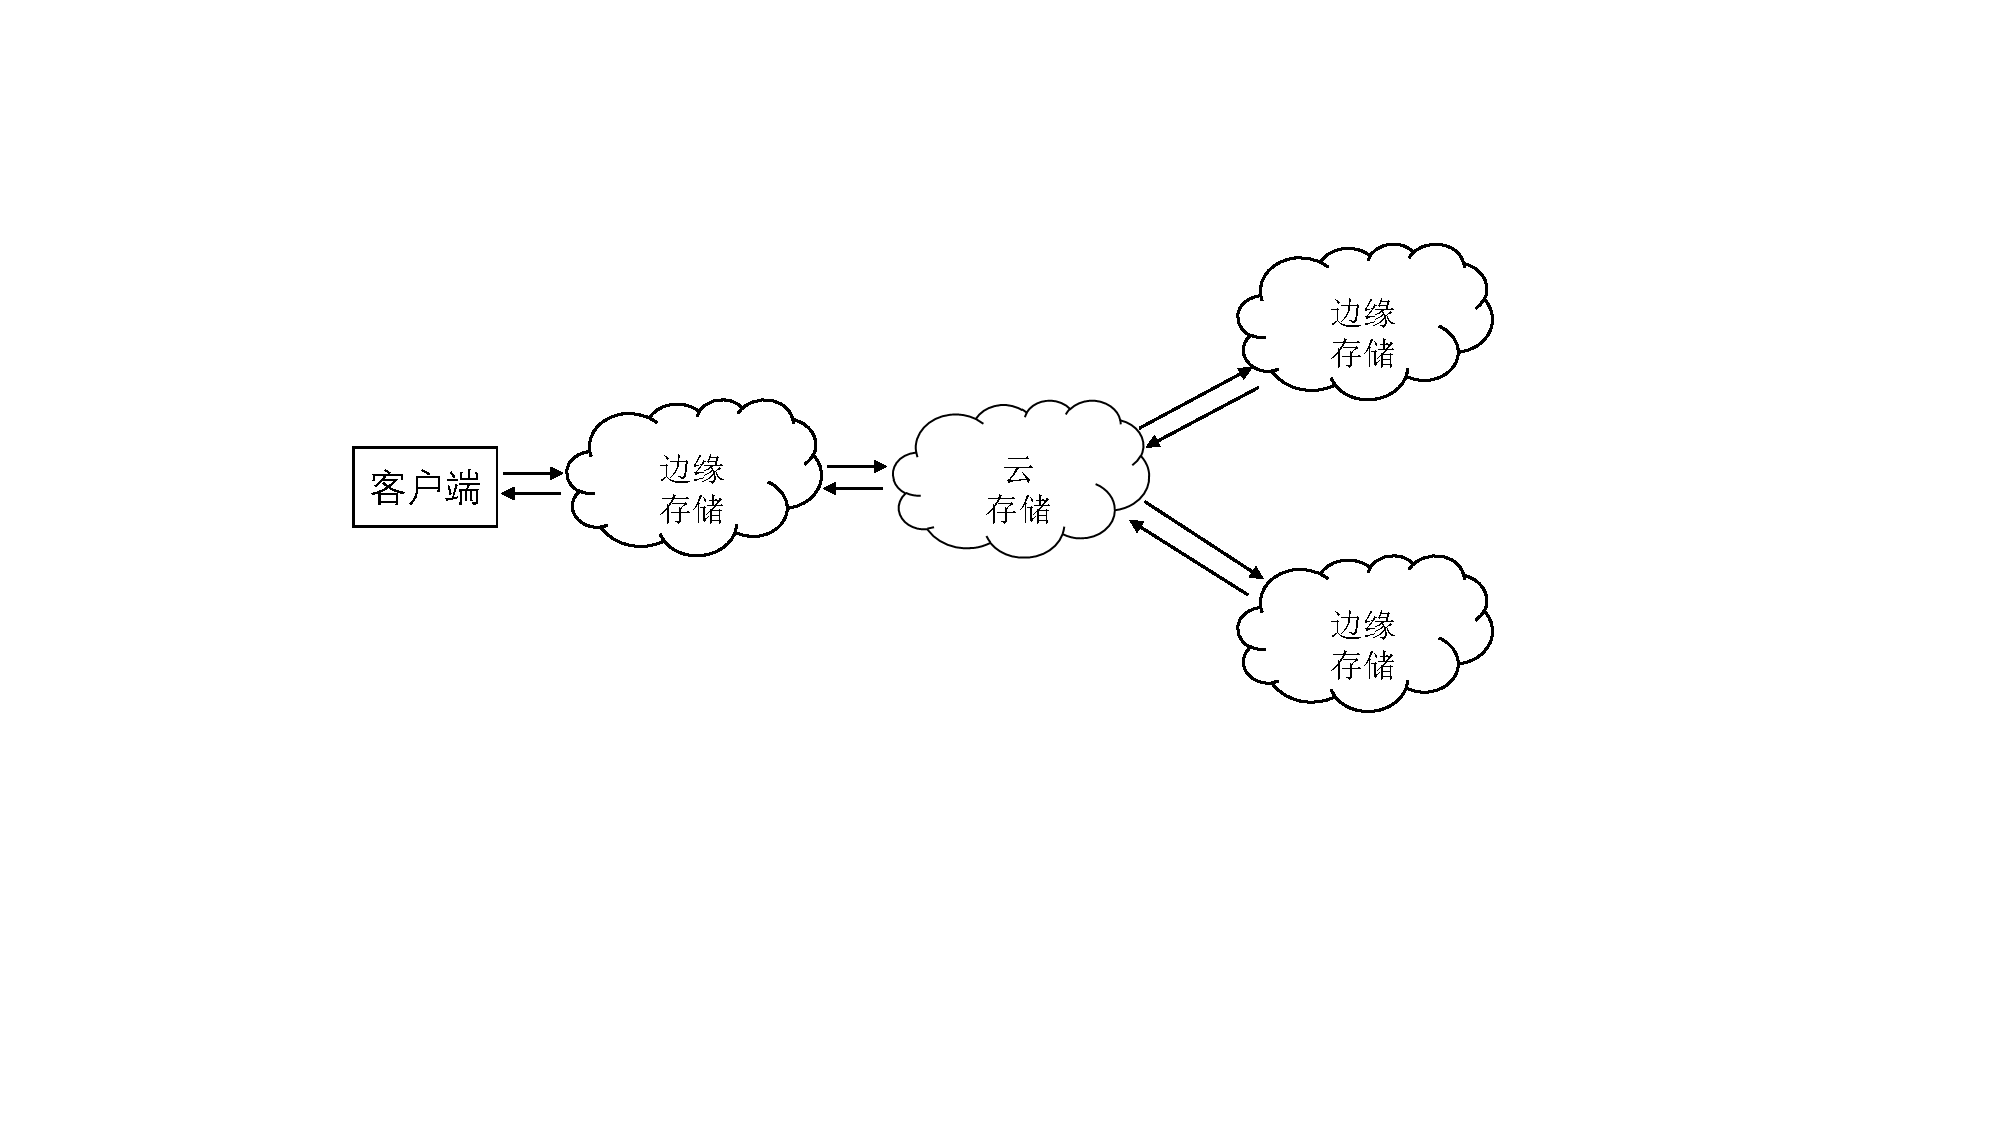
\includegraphics[width = 1.0\linewidth]{pic/miwenjiansuoliuchengtu.pdf}
    \caption{密文检索流程图}
    \label{密文检索流程图}
\end{figure}

在密钥更新时,用户端下载密文文件的一小部分(基于CAONT加密方案生成的小部分数据),更新密钥之后加密之后重新上传至边缘服务器,这个时候边缘服务器会有选择的上传新数据至云服务器。

在下载数据文件时,倘若用户端想要下载与其同边缘服务下的其他用户的数据文件,那么边缘服务器直接传输数据块和元数据给用户端,用户端根据元数据信息拼接并解密成明文文件;倘若用户端要下载的文件是其他边缘服务下的,那么满足一定的权限下(基于密文策略属性基加密方案\citing{bethencourt2007ciphertext}实现权限管理和认证),云存储会将数据块及相应元数据传输给该用户端的边缘服务器,边缘服务器再传输给目标用户端。

本论文的系统采用这种架构模型,旨在实现以下几点目标:

1)存储上的低开销。往往来源于同一个机构的文件级重复度相对较高\citing{chen2015bl},所以在边缘服务器上采用文件级别的去重保障一定的存储低开销;在中心化的云服务上进行数据块级的去重保障了来源于不同边缘服务器的数据的存储低开效。

2)响应多用户的高吞吐量。在每一个边缘服务器上,采用文件级去重,并保障来源于同一个文件的密文数据块顺序存储在磁盘上。众所周知,磁盘的顺序读写性能远远高于随机读写。这种架构方式充分利用磁盘的顺序读写性能,无论在响应多用户的上传文件(磁盘写)还是下载文件(磁盘读)方面,都能达到较高的响应速度。

3)关键词检索的局部性和全局性统一。关键词关联信息存在一定的局部性,边缘服务器存放相关局部性特征。此外,全局的云服务器也会充当边缘服务器密文关键词检索的客户端,向四周的边缘服务发起该关键词检索的关联信息检索,收集并一起推送给用户所在边缘服务器。

4)一定程度的容灾备份。本论文的密文去重系统目前只涉及服务器逻辑层面的功能,即无论边缘服务器还是云服务对外提供服务都是以逻辑机器服务提供出去。\ref{展望}会接着探讨物理机器层面的高可用以及机器分片的高性能。即便如此,本论文的密文去重系统毅然存在一定程度的容灾备份效果:云服务器作为全局的中心服务器,备份存储了来源于各个边缘服务器的数据块,也就是说每一个密文数据块至少存在了两个副本,其中一个是云服务上经过去重之后的副本,还有至少一个副本存放在边缘服务器顺序存储的磁盘上。
\section{威胁模型}
本论文假设存在一个诚实且好奇(honest-and-curious)的敌手,他致力于获取外包存储服务上文件的内容。这个敌手可以采取以下攻击措施:

1)敌手能够攻陷服务器,并且能够访问存放在服务器上所有的数据块和秘钥。

2)敌手能够与一些未授权或权限撤销的客户端密谋,并且尝试学习超出合谋客户端的访问范围的文件。

3)敌手可以监视客户端的申请MLE密钥活动,识别密钥管理器返回的MLE密钥,并提取被监视客户端拥有的文件。

4)敌手监听客户端的密文检索活动,根据检索同一个密文关键词的频率以及文件唯一标识符等信息,推断出其他超出范围的信息。

本论文对威胁模型做出以下假设:

1)本论文假设为了抵御网络通信活动中的窃听风险,客户端和密钥管理器间的通信是经过加密和认证的(例如,使用SSL/TLS)。每个客户端和密钥管理器采用模糊密钥生成技术\citing{keelveedhi2013dupless},所以密钥管理器不能推断出指纹信息和学习信息内容。

2)本论文假设密钥管理器部署在一个完全受保护的环境,并且任何敌手不能攻陷或者获取密钥管理器的访问权限。

本论文不考虑敌手从受损客户端对密钥管理器发起在线暴力攻击的威胁,因为密钥管理器会对每一个客户端的查询速率进行速率限制\citing{keelveedhi2013dupless}。本论文的系统可以和远程数据检查\citing{ateniese2007provable, juels2007pors}结合部署来高效检测外包数据的完整性、抵御恶意数据破坏。由于本论文的系统采用的是服务端去重,它不会在数据去重中引入辅助通道(side-channel),因此也不存在辅助通道攻击。

最后,本论文的系统聚焦于三个主要的安全性目标:

1)系统保证机密性,所以密文数据块的内容不能被任何城市且好奇的敌手(例如,任何未授权的用户或服务端)窥探到。此外,系统阻止被撤销权限的用户访问和更新任何存放于服务端的文件。

2)系统保证完整性,所以当一个客户端下载一个数据块时可以检测数据是否完整。

3)本文的密文关键词检索功能并具备传统对称可搜索加密的安全性\citing{curtmola2006searchable},而是以“尽可能强的安全性”(as strong as possible  security strength)为目标的\citing{wang2011enabling}。也就是说,为了功能性和高效性,本系统会对有些关键性信息以明文形式存放于服务器。但是,这不代表这密文检索功能完全不安全。


\section{兼容密钥更新的安全高效密文去重方法}\label{CAONT}
本系统的安全性是同时建立在两个对称加密密钥上的:每一个文件的文件级密钥(简称文件密钥)和每一个数据块的MLE密钥(简称MLE密钥)。在密钥更新期间,系统只需要更新密文密钥而所有数据块的MLE密钥保持不变。本论文认为这种重新加密方案实现了安全目标,同时保持了数据去重的高效性,并允许在权限撤销中进行轻量级重新加密。

\subsection{基于CAONT的数据加密和密钥更新技术}\label{基于CANOT的数据加密和密钥更新技术}
本论文提出了两种加密方案:基本加密方案和增强加密方案。基本加密方案更高效但容易遭受MLE密钥泄漏的攻击;增加加密方案阻止了MLE密钥的泄漏同时也引入了额外的加密步骤。在阐述两种加密方案之前,先简单叙述CANOT技术。

\textbf{CAONT技术}

本系统是采用CAONT(Convergent All-or-Nothing Transform)技术作为基础加密原语的,CAONT技术可以视为\acrshort{AONT}(All-or-nothing)技术的变种。为了整篇论文逻辑的完整性,本章节会简单交代AONT技术的要点,然后再阐述CAONT技术的创新点,最后总结本系统基于CAONT原语的原因。

AONT技术\citing{rivest1997all}将一个明文信息$M$转换成一个数据包$(C, t)$,其中$C$代表数据包的头部,$t$代表数据包的尾部。具体来说,首先选择一个随机的加密密钥$K$并且产生一个随机掩码$G(K) = E(K, S)$,其中$E(\cdot)$代表一个对称加密函数(例如,AES-256)且$S$是一个公开的、和明文$M$有相同大小的数据块。然后计算$C = M \oplus G(K)$,此处‘$\oplus$’代表异或(XOR)操作符,并且计算$t = H(C) \oplus K$,其中$H(\cdot)$是一个哈希函数(例如,SHA-256)。这样计算出来的结果数据包比原始数据$M$多了$t$。为了计算出原始明文$M$,假设已知数据包$(C, t)$,可以先计算出$K = H(C) \oplus t$,然后计算出$M = C \oplus E(K, S)$。

CAONT\citing{li2015cdstore}技术和以上ANOT技术具有相同的加解密逻辑,但是使用确定的、来源于明文$M$的哈希信息$h = H(M)$作为随机的加密密钥$K$。这样使得相同的密文信息会产生内容相同的数据包,因此使得密文去重成为可能。CAONT技术的另一个特性是,它允许在没有填充的情况下进行完整性检查。具体来说,在恢复数据包之后,可以通过计算明文$M$的哈希值来检查其是否等于$h$来验证完整性。

AONT是一种未知的随机加密模式,它将消息转换为称为密文数据包,其属性是:在不知道整个包的情况下,在计算上基本不可能还原成原始消息。原生的AONT设计阻止了数据去重,因为它的转换将随机密钥作为构建密文数据包的输入。而CAONT技术用确定性消息派生密钥替换随机密钥来构建密文数据包,这确保了相同明文总能加密生成相同的密文包。

\textbf{基础加密方案}\label{caont-basic}

基础加密方案运用CAONT技术产生两个密文部分:修剪包(trimmed package)和存根(stub)。实际上,本论文对CAONT方案做了两个地方修改。第一个修改是数据加密密钥方面:从用哈希函数提取明文信息的哈希值作为加密密钥的方式转变成由密钥管理器生成MLE密钥的方式。这个思路借鉴了DupLESS\citing{keelveedhi2013dupless}系统,其中密钥管理器生成密钥的方式有两点好处:\ding{172}密钥管理器采用盲签名机制协助客户端基于明文哈希值生成MLE密钥,规避离线暴力字典攻击;\ding{173}密钥管理器执行严格的客户端请求MLE密钥生成速度,有效抵抗在线暴力字典攻击。然而,第一个修改会使得系统不能使用哈希值去验证数据的完整性。因此,本论文又增加了第二个修改点:在原始明文数据$M$中追加一个公知的、固定大小的数据$c$,称为“金丝雀”。在明文数据块加密再解密之后,可以校验“金丝雀”$c$是否发生改变并以此来验证数据的完整性。
% \begin{figure}[htbp]  
%     \centering  
%     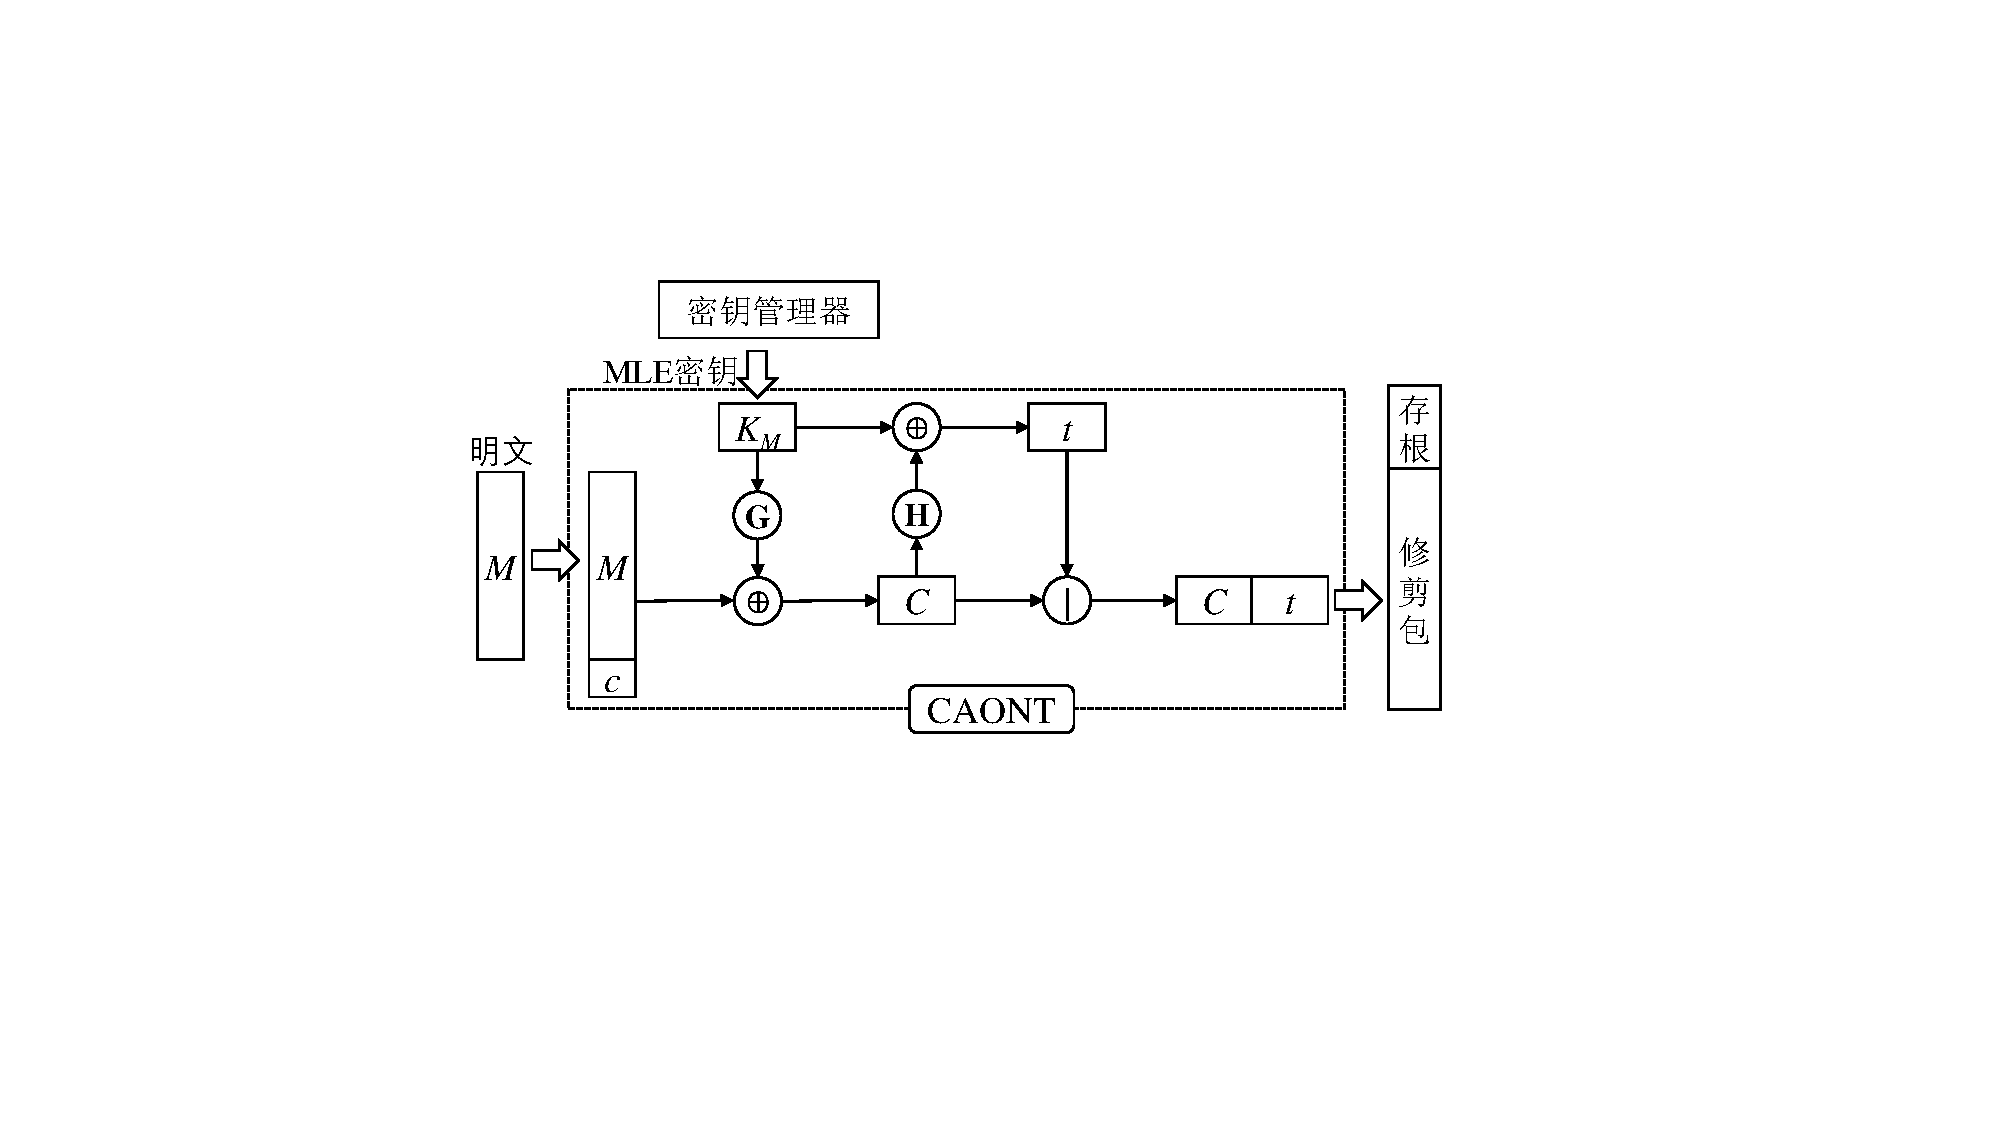
\includegraphics[width = 0.8\linewidth]{pic/基础加密图}  
%     \caption{基础加密方案} 
%     \label{基础加密方案}  
% \end{figure}
%不画图

基础加密方案详细流程如下:

1)首先,拼接明文块$M$和“金丝雀”$c$生成$(M||c)$并作为一个整体参与后续计算,计算伪随机掩码$G(K_M) = E(K_M, S)$,此处$K_M$是从密钥管理器获取的MLE密钥并且$S$是一个公知的、和$(M||c)$具有相同大小的数据块。

2)然后,计算数据包的头部$C = (M||c) \oplus G(K_M)$,此处‘$\oplus$’是异或(XOR)操作符,计算数据包的尾部$t = K_M \oplus H(C)$。

3)最后,将数据包的头部和尾部拼接在一起形成整个数据包,并选取整个数据包的最后的若干字节(例如,64字节)的数据作为存根(stub),将剩余的部分称为修剪包(trimmed package)。

将文件的所有数据块的存根(stub)使用用户选定的文件密钥加密,并上传外包服务端。这样,数据块大部分内容(即修剪包)都能加密成相同密文支持密文数据去重,而只有少部分内容(即存根)由用户指定文件密钥加密而不能参与去重但却能被用户更新密钥而重加密。因为重加密的部分是来源于每一个数据块的极少部分(即存根),所以重加密的速度理论上来说要比重加密整个数据块提升很大,与此同时,因重加密而上传下载文件的网络带宽也会得到极大的节约。

基础加密方案很容易受到MLE密钥泄漏攻击。具体来说,敌手在攻破某一个客户端之后会监听由密钥管理器生成的MLE密钥(即上文中的$K_M$)。如果一个MLE密钥泄漏,那么敌手很容易能发现伪随机掩码(即上文中的$G(K_M)$)并用该掩码和密文中修剪包做异或(XOR)操作获取数据块中大部分内容。

\textbf{增强加密方案}\label{caont-enhanced}

由于基础加密方案存在MLE密钥泄漏攻击问题,所以本论文进一步设计了安全性增强的加密方案,其中方框中内容代表数据(包括明文或密文)或者组件,圆圈和椭圆中符号代表运算符,箭头代表运算流程方向。增强加密方案的工作流程中首先运用密钥管理服务器的MLE密钥生成MLE密文,再将CAONT技术运用到整个MLE密文上。其底层原理在于因为MLE密文被CAONT保护着,即使敌手攻破了MLE密钥,仍不能恢复原始的明文数据块。
% \begin{figure}[htbp]  
%     \centering  
%     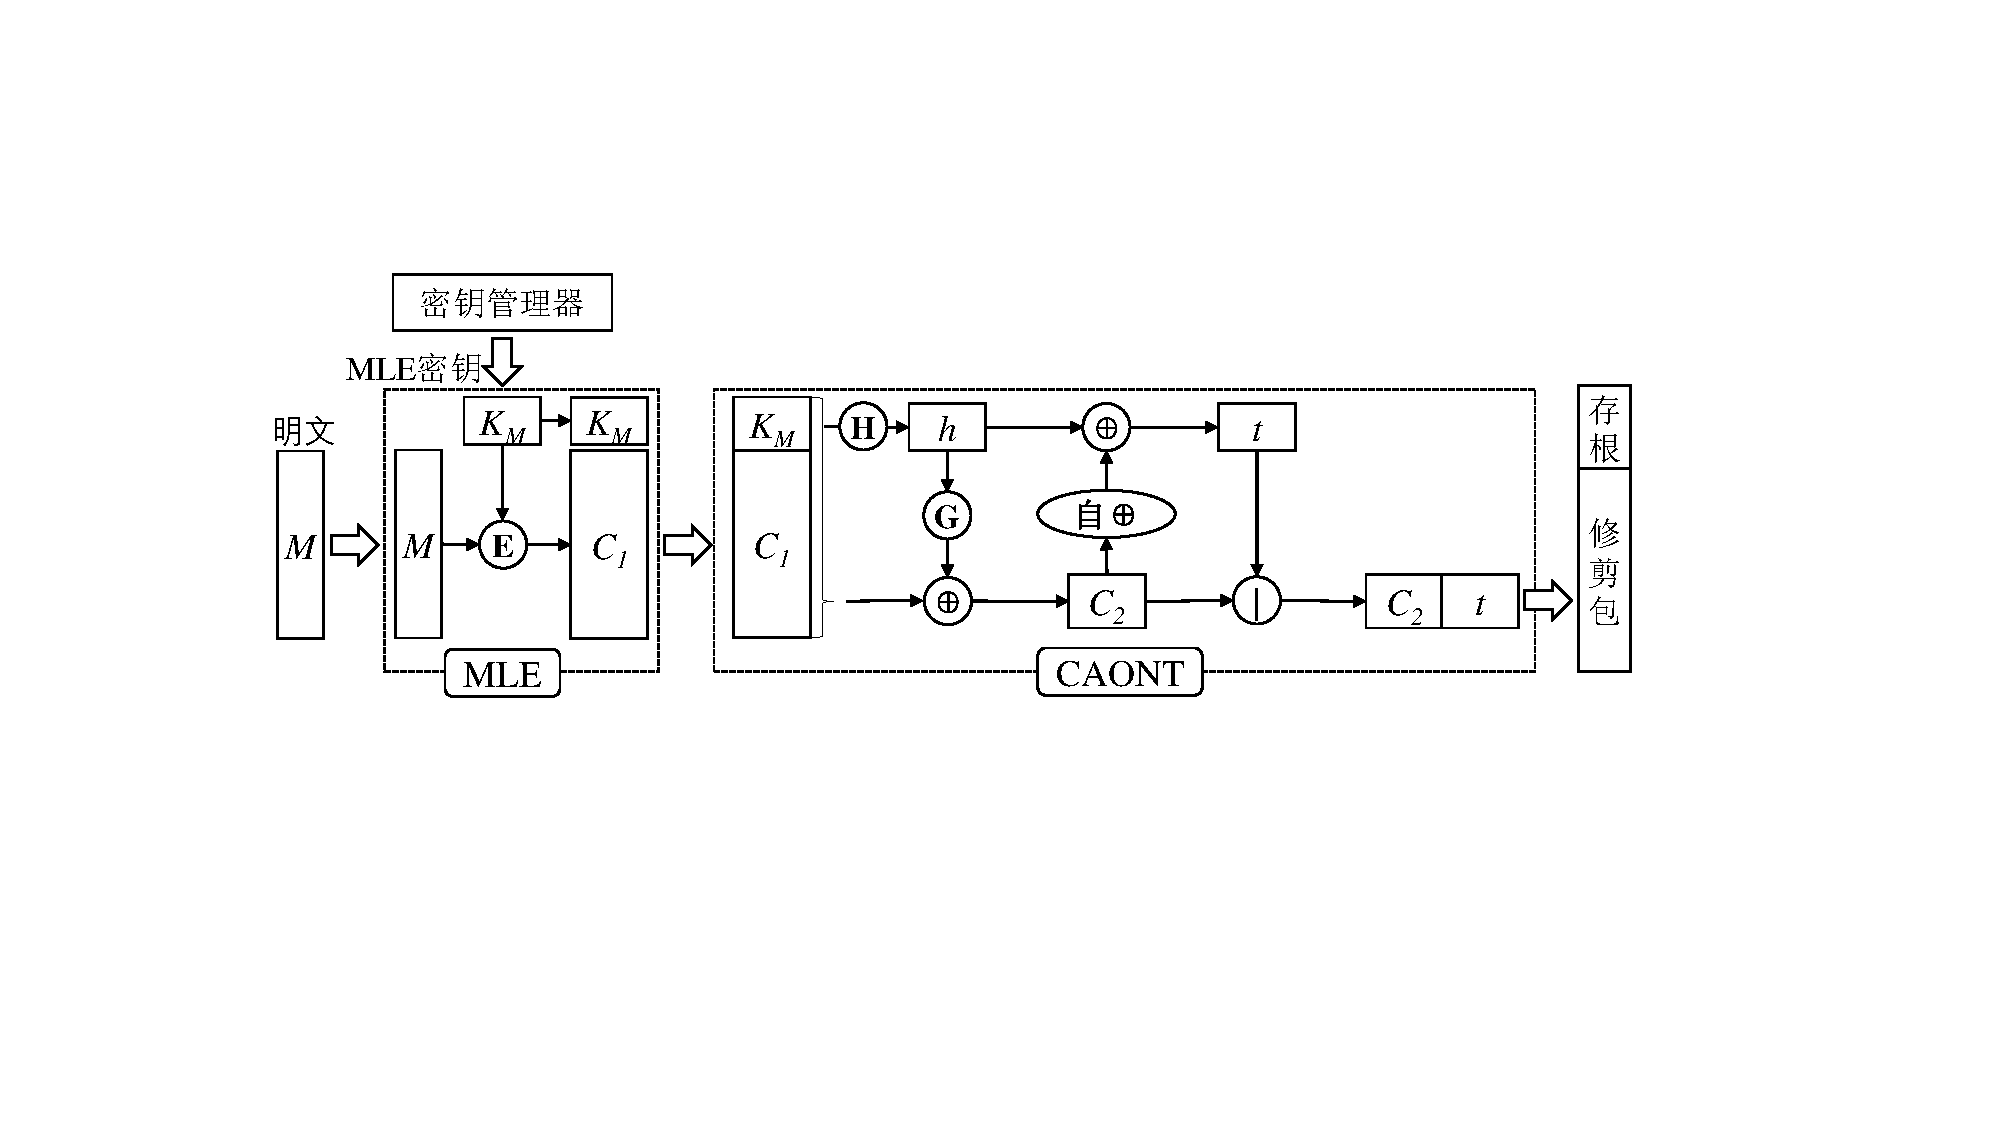
\includegraphics[width = 1.0\linewidth]{pic/增强加密图}  
%     \caption{增强加密方案} 
%     \label{增强加密方案}  
% \end{figure}
%不画图

增强加密方案细节描述如下:

1)首先,像基础加密方案一样,从密钥管理器获取的MLE密钥$K_M$,使用$K_M$加密一个输入的数据块并且获取密文$C_1$。

2)然后,基于原始的CAONT技术对结合体$C_1||K_M$进行转换。本论文并没有采用基础加密方案中的MLE密钥而是采用哈希值$h =  H(C_1||K_M)$去转换数据包,这样就可以规避使用CAONT技术转换强依赖MLE密钥安全性的风险。严谨地说,本文计算哈希值$h = H(C_1||K_M)$和伪随机掩码$G(h) = E(h, S)$,此处$S$是一个公共知晓的、和$C_1||K_M$具有相同大小的数据块,然后计算机数据包的头部$C_2 = (C_1||K_M) \oplus G(h)$。

3)最后,由于可以使用哈希值$h$可以检测数据的完整性,为了高效,本论文并没有使用基础加密方案中对密文运用哈希运算而是采用自抑或的操作来产生数据包的尾部$t$。具体来说,均等地将$C_2$分为一组和$h$具有相同大小的数据块,然后异或操作所有的数据块以及$h$得到数据包的尾部$t$。当不知道整个$C_2$的内容时,自异或的结果并不能被预测到。本论文采用和基础加密方案中类似的方法从$(C_2, t)$中截取修剪包和存根。

为了恢复明文$M$,首先要从修剪包和存根中恢复$(C_2, t)$,将$C_2$部分均等地分成若干个和$t$相等大小的数据块并异或操作所有的数据块和$t$得到$h$。然后,通过计算$C_2 \oplus G(h)$得到$C_1||K_M$,并通过比较$H(C1||K_M)$和$h$校验数据的完整性。最后,计算$M = D(K_M, C_1)$,此处$D(\cdot)$是解密函数并且解密密钥是上文中的MLE密钥。

同样地,客户端会使用用户指定的文件密钥对存根部分数据进行再加密。当用户需要密钥更新时,也只需要下载少部分数据(即所有的存根)并进行重加密,大大节约网络通信和CPU计算的开销。

\subsection{基于相似性密钥生成技术}
\ref{基于CANOT的数据加密和密钥更新技术}章节交代了数据块加密和密钥更新的详细流程,然而,若只将外包数据切分成若干数据块并对每一个数据块进行如上的加密操作存在很明显的性能瓶颈:密钥管理器辅助生成MLE密钥造成极大的系统负载。

本论文的实验研究发现,密钥管理器辅助生成MLE密钥必须为每个数据块执行RSA盲签名算法(见\ref{RSA盲签名},一个RSA盲签名算法包括盲化、签名和去盲化)\citing{keelveedhi2013dupless},造成极大系统负载。在千兆网环境下,为一个8KB的数据块生成MLE密钥需要时间1125.3$\upmu$s,其中盲化用时46.3$\upmu$s,签名用时537.2$\upmu$s,去盲化用时246.9$\upmu$s,密钥传输用时294.9$\upmu$s。换句话来说,数据吞吐量是8KB / 1125.3$\upmu$s $\approx$ 6.9MB/s,远低于千兆网络的传输速率(1Gb/s$\approx$128MB/s)。导致该瓶颈的主要原因是RSA盲签名,因为盲化、签名和去盲化操作占了密钥生成的总延迟的73.8\%,见图\ref{服务器辅助生成MLE密钥各步骤占比}。

\begin{figure}[htbp]
    \centering
    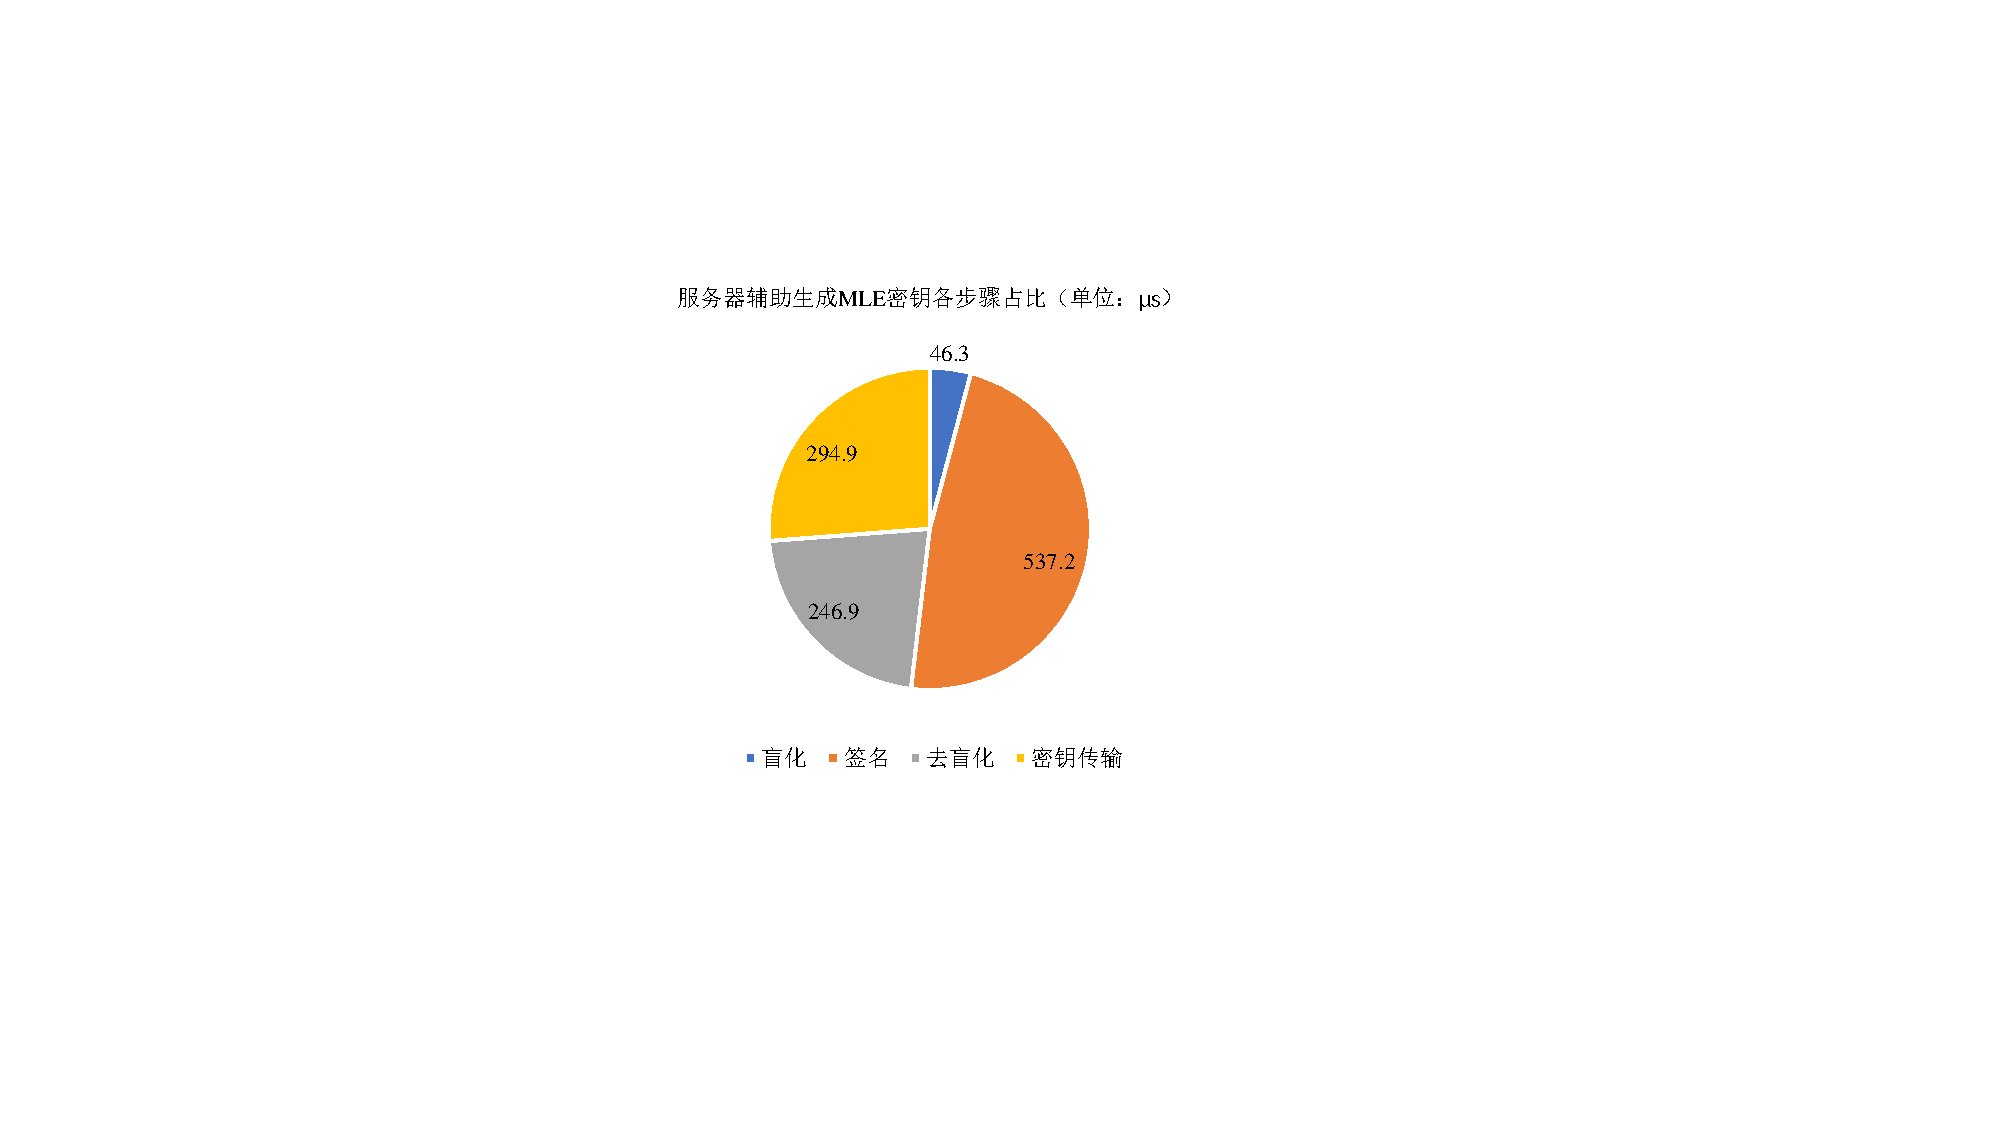
\includegraphics[width = 0.55\linewidth]{pic/服务器辅助生成MLE密钥各步骤占比.pdf}
    \caption{服务器辅助生成MLE密钥各步骤占比}
    \label{服务器辅助生成MLE密钥各步骤占比}
\end{figure}

\begin{comment}

\end{comment}

本论文提出了基于相似性的密钥生成技术,其核心思想是:将若干个相邻的数据块聚合在一个数据片段里面(segment),并针对每一个数据片段只会向密钥管理器申请一次MLE密钥,大大缩减了密钥生成次数来提高数据的吞吐量;在生成数据片段级MLE密钥时,本论文选用每一个片段中所有数据块哈希值的最小值作为整个片段所有数据块的代表值,以此向密钥管理服务器申请MLE密钥,从而保证了来自于同一个数据片段的数据块会有相同的MLE密钥并被加密成相同的密文数据块支持密文去重,同时,来源于不同数据片段的相同数据块可能由于MLE密钥不同会被加密成不同的密文块。换句话说,相似性密钥生成方案中密文去重分为两种情况:\ding{172}同一个数据片段中的相同数据块间的去重(片段内去重,不妨叫情况1);\ding{173}不同数据片段中相同数据块并且因为选取的代表块一样而被加密成相同的密文数据块支持去重(片段间去重,不妨叫情况2)。此外,还有一种被忽略的不能支持去重的情况:来自于不同数据片段的相同数据块,但是数据片段选取的代表数据块不同而被加密成不同的数据块密文而不支持去重(片段间无法去重,不妨叫情况3)。

图\ref{基于相似性的密钥生成方案示例}描述了基于相似性的密钥生成技术的一个实例:将输入流按照相邻4个数据块聚合成一个数据片段,作为密钥生成的基本单位,然后从中选取最小的数据块作为申请MLE密钥的代表块。其中,字母A,B,C,D,E代表着每一个数据块的哈希值并且A代表着最小哈希值,E代表着最大哈希值,阴影块代表最小块(即代表块),反斜杠“$\backslash$”代表着支持去重的数据块。对于分段1,采用A作为整个分段的哈希值代表向密钥管理器申请MLE密钥,并分别对四个数据块进行\ref{CAONT}章节中所描述的方式加密。分段2和3采取相同的措施申请MLE密钥并加密数据块。分段1中四个数据块均不相同,均不符合情况1和2,所以不能支持数据片段中去重;分段2中的数据块D和E符合情况2,所以能支持片段内的去重;分段3的数据块A、B和C符合情况2,能支持片段间的去重,也就是说分段3和分段1都是以数据块A作为代表块申请MLE密钥进行加密,那么两个分段中的相同的明文块被加密成相同的密文块支持去重,但是由于分段3的数据块E和分段2的数据块E属于情况3而不支持去重。
\begin{figure}[htbp]
    \centering
    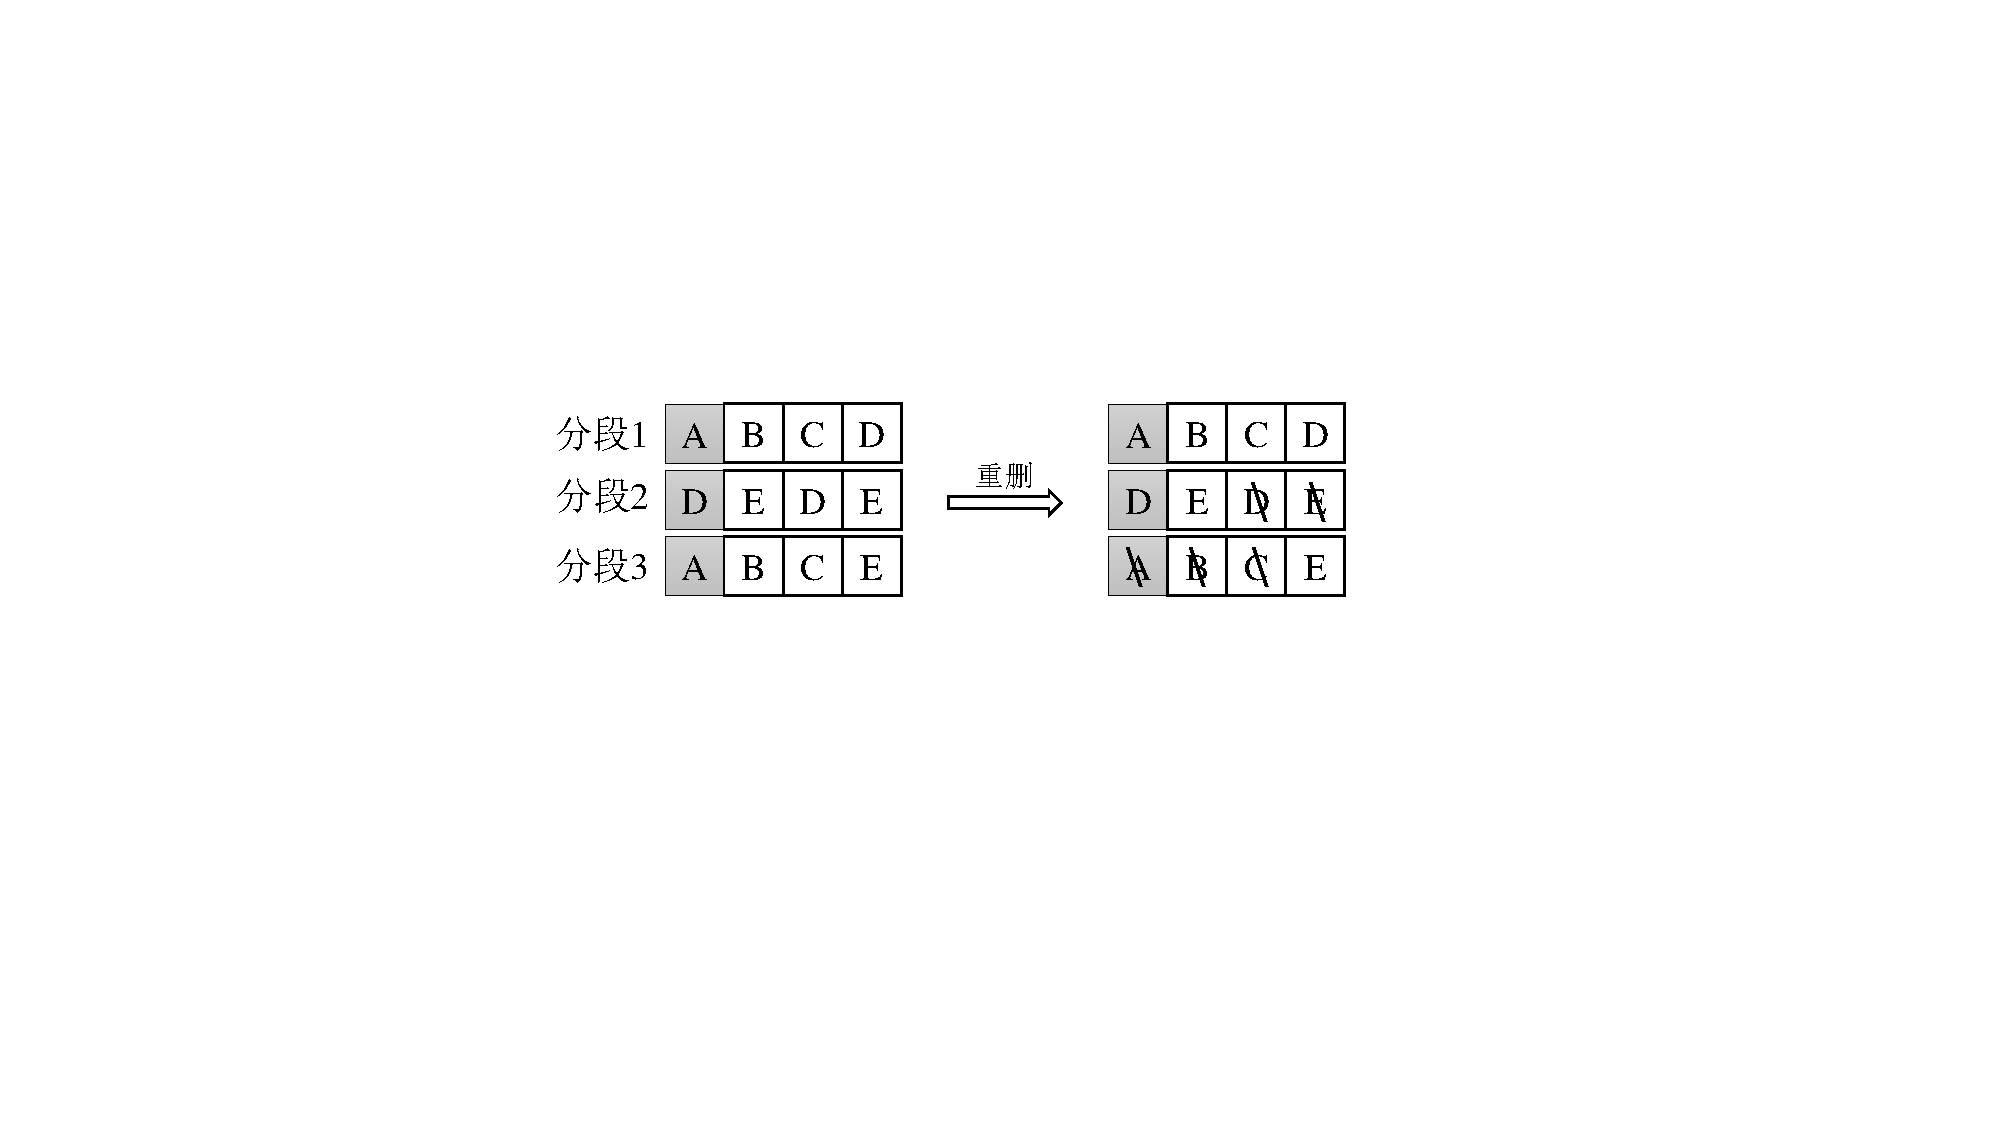
\includegraphics[width = 0.6\linewidth]{pic/相似性密钥生成方案.pdf}
    \caption{基于相似性的密钥生成方案示例}
    \label{基于相似性的密钥生成方案示例}
\end{figure}

基于相似性密钥生成技术中选择最小哈希值作为片段代表性哈希值的理论依据是Broder定理\citing{broder1997resemblance}:将两个集合的相似度系统定义为两个集合所包含元素的最小哈希值相等的概率。当数据集具备良好的局部性特征时,具有较多的相同的数据块的数据片段(即相似数据片段)往往都有相同的最小哈希值,因此来源于不同数据片段的相同数据块被加密成不同的密文数据块的几率是可以忽略的(即情况3是可以忽略的),也就是说在这些数据分段之间执行数据去重操作能够达到接近于数据块级别去重的存储开销。本论文的实验表明,基于相似性的密钥生成技术可以将数据块级别的密钥生成速率从11.8MB/s提升至167.6MB/s,但只会降低至多0.3\%的存储空间开销。

\subsection{支持懒惰更新的动态访问控制技术}\label{支持懒惰更新的动态访问控制技术}
\ref{基于CANOT的数据加密和密钥更新技术}中提及对密文的进行密钥更新时,只是用新的文件级密钥(file key)对密文数据块的存根部分(stub)进行重新加密。那么,文件级密钥又是如何更迭的呢?本章节会做详细阐述。

首先,笼统地讲,本章节的动态访问控制技术是基于两个现有的密码学原语的:基于密文策略的属性基加密(Ciphertext-policy Attribute-Based Encryption,CP-ABE)和密钥回归技术(Key Regression)。所以在讲解核心技术点之前阐述一下这两个密码学原语。

\textbf{属性基加密}\label{属性基加密}

为了细粒度的共享加密数据和细粒度的访问控制,加密存储系统往往会融入属性基加密技术。在本论文中,考虑到现实架构下的需要给特定的用户组不同权限场景,系统中细粒度权限授予和撤销等相关功能需要借用基于密文策略的属性加密技术(Ciphertext-policy Attribute-Based Encryption,CP-ABE),本章节对该技术进行简要叙述。

基本属性基加密(Attribute-Based Encryption)机制源于基于模糊身份的加密(Fuzzy Identity-Based Encryption,FIBE)方案\citing{sahai2005fuzzy},该方案首次提出用一组属性来描述用户身份。基本属性方案被划分成基于密钥策略的属性基加密(Key-policy Attribute-Based Encryption,KP-ABE)\citing{goyal2006attribute}和基于密文策略的属性基加密(Ciphertext-policy Attribute-Based Encryption,CP-ABE)\citing{bethencourt2007ciphertext}。前者是将策略嵌入到密钥中,属性嵌入到密文中,往往被应用在付费视频网站和日志加密管理中;后者是将策略嵌入到密文中,属性嵌入到密钥中,往往被应用在数据加密存储和细粒度共享中。

在CP-ABE方案中,访问树用于隐藏源数据的加密密钥,其形状结构如其名一样,是一颗树。其叶子节点为数据所有者设定的属性和属性值以及父节点传于此节点的秘密值,并对其进行加密处理,只有数据访问者拥有此属性方可解密此节点的秘密值;非叶子节点为门限节点,数据访问者需满足此门限最低值方可解密此节点秘密值,例如门限为3/5,此节点有5个子节点,数据访问者需要至少满足三个子节点才能解密出秘密值。如图\ref{CP-ABE的访问树例图},这是一个访问树例图,只有当用户的属性满足根节点的两个以上子节点才能解开根节点中存放的消息密文。例如,用户Alice的属性集描述为\{计算机学院、硕士、研二、云实验室\},那么前三个属性满足“3/3”这个非叶子节点的门限要求,最后一个属性“云实验室”能满足“1/2”这个非叶子节点的门限要求,所以Alice满足根节点的门限要求。

\begin{figure}[htbp]
    \centering
    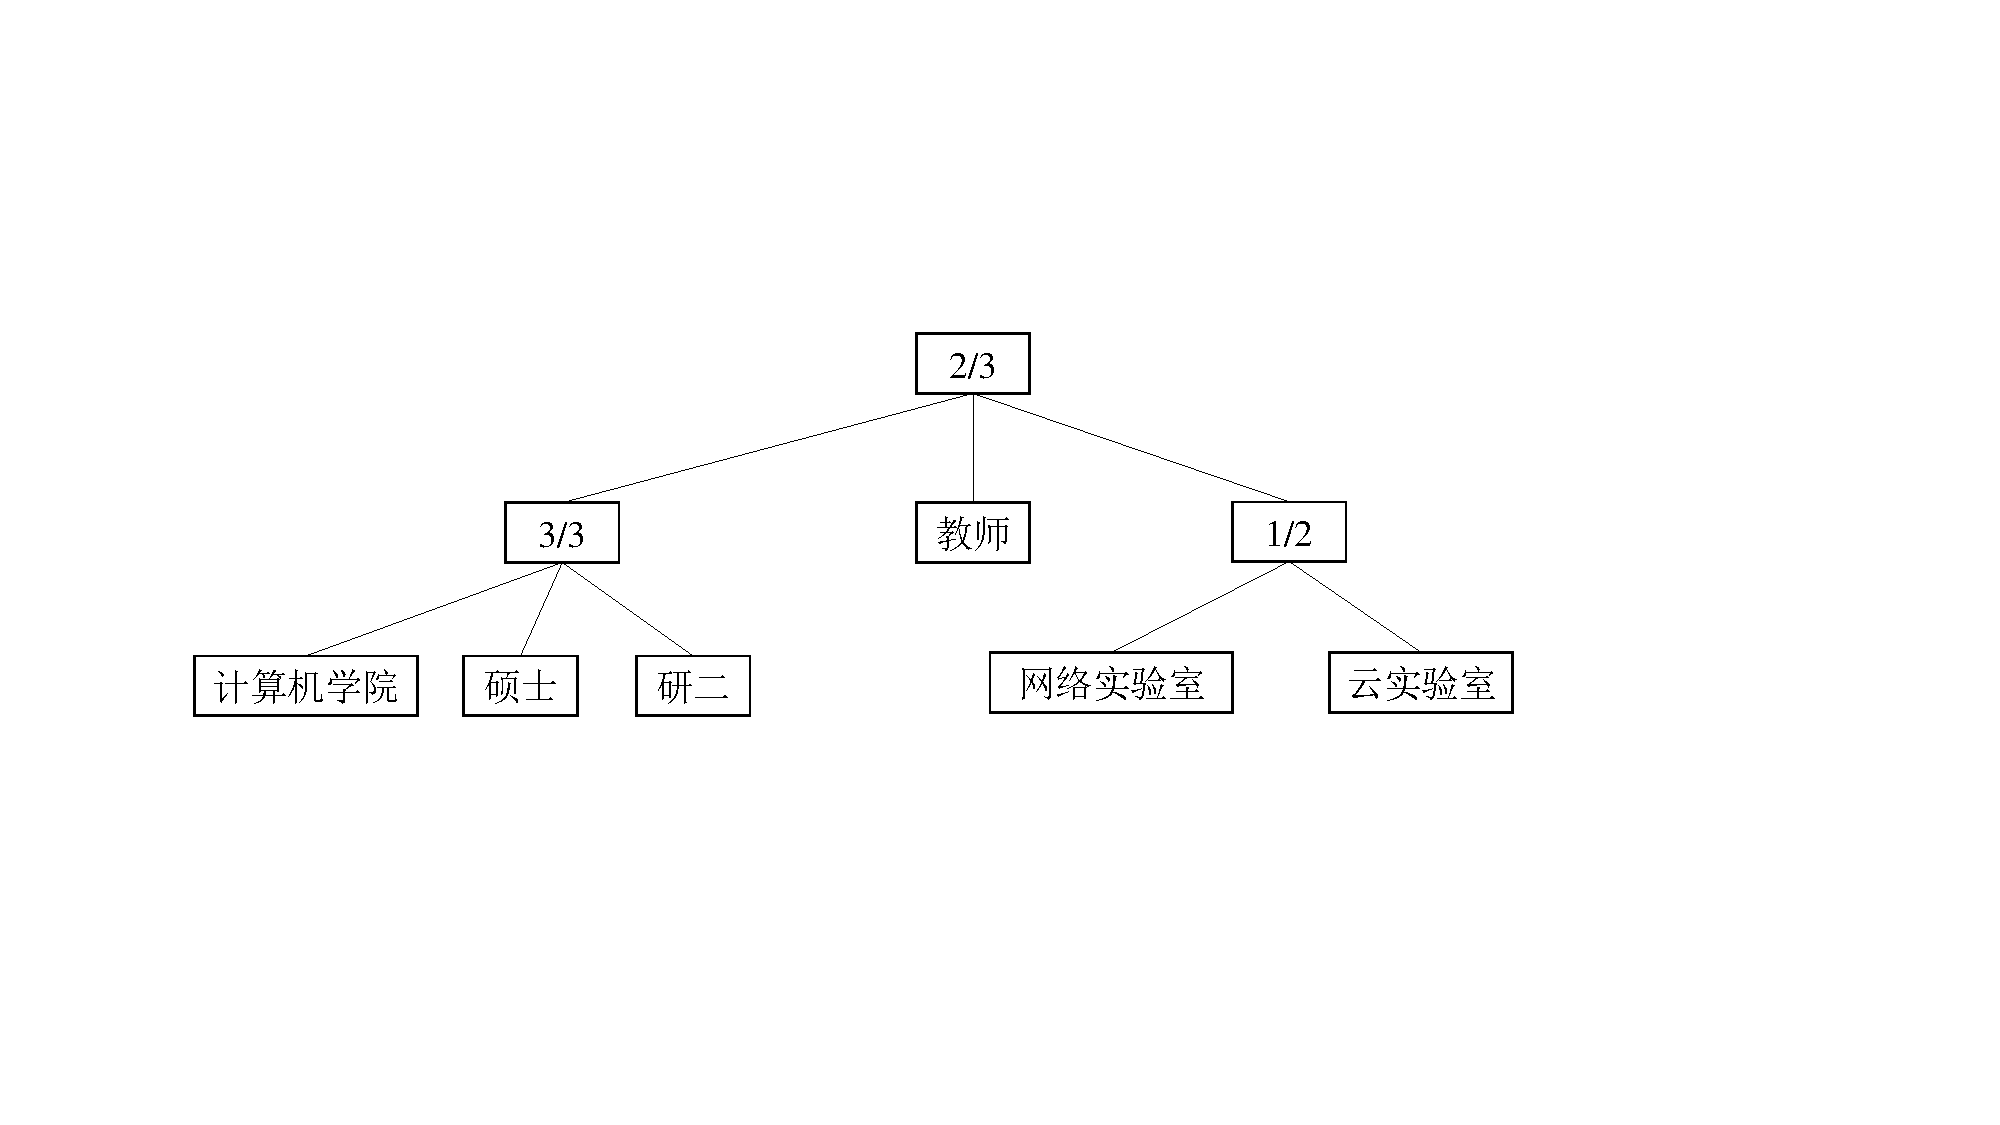
\includegraphics[width = 0.9\linewidth]{pic/基于密文策略的属性基加密例图.pdf}
    \caption{CP-ABE的访问树例图}
    \label{CP-ABE的访问树例图}
\end{figure}

本章节旨在用通俗简易的语言交代CP-ABE的核心思想,为支持懒惰更新的动态访问控制技术中新技术点的研究打下良好铺垫。CP-ABE的详细算法流程以及数学原理可参考\cite{bethencourt2007ciphertext}。

\textbf{密钥回归}\label{密钥回归}

密钥回归(Key Regression)\citing{fu2006key}是一种解决内容分发网络(Content Distribution Network,CDN)上从最近的密钥中导出一系列与时间相关的密钥的方法技术,源于Plutus文件系统中的密钥轮换技术(Key Rotation)。密钥回归技术弥补了密钥轮换技术存在的不安全性,常常被内容分发网络应用来降低内容发布者在实际工作下的带宽需求。本论文中系统的支持懒惰更新的动态访问控制技术需要基于密钥回归技术,并对密钥回归技术做了很好的扩展和应用。

密钥回归技术框架中有多个重要的变量和函数:$stp_i$代表第$i$个内容发布者状态值;$stm_i$代表代表第$i$个成员状态值;$K_i$代表第$i$个成员所拥有的密钥值;三个单向不可逆的函数$wind$、$unwind$和$keyder$。

% \begin{figure}[htbp]  
%     \centering  
%     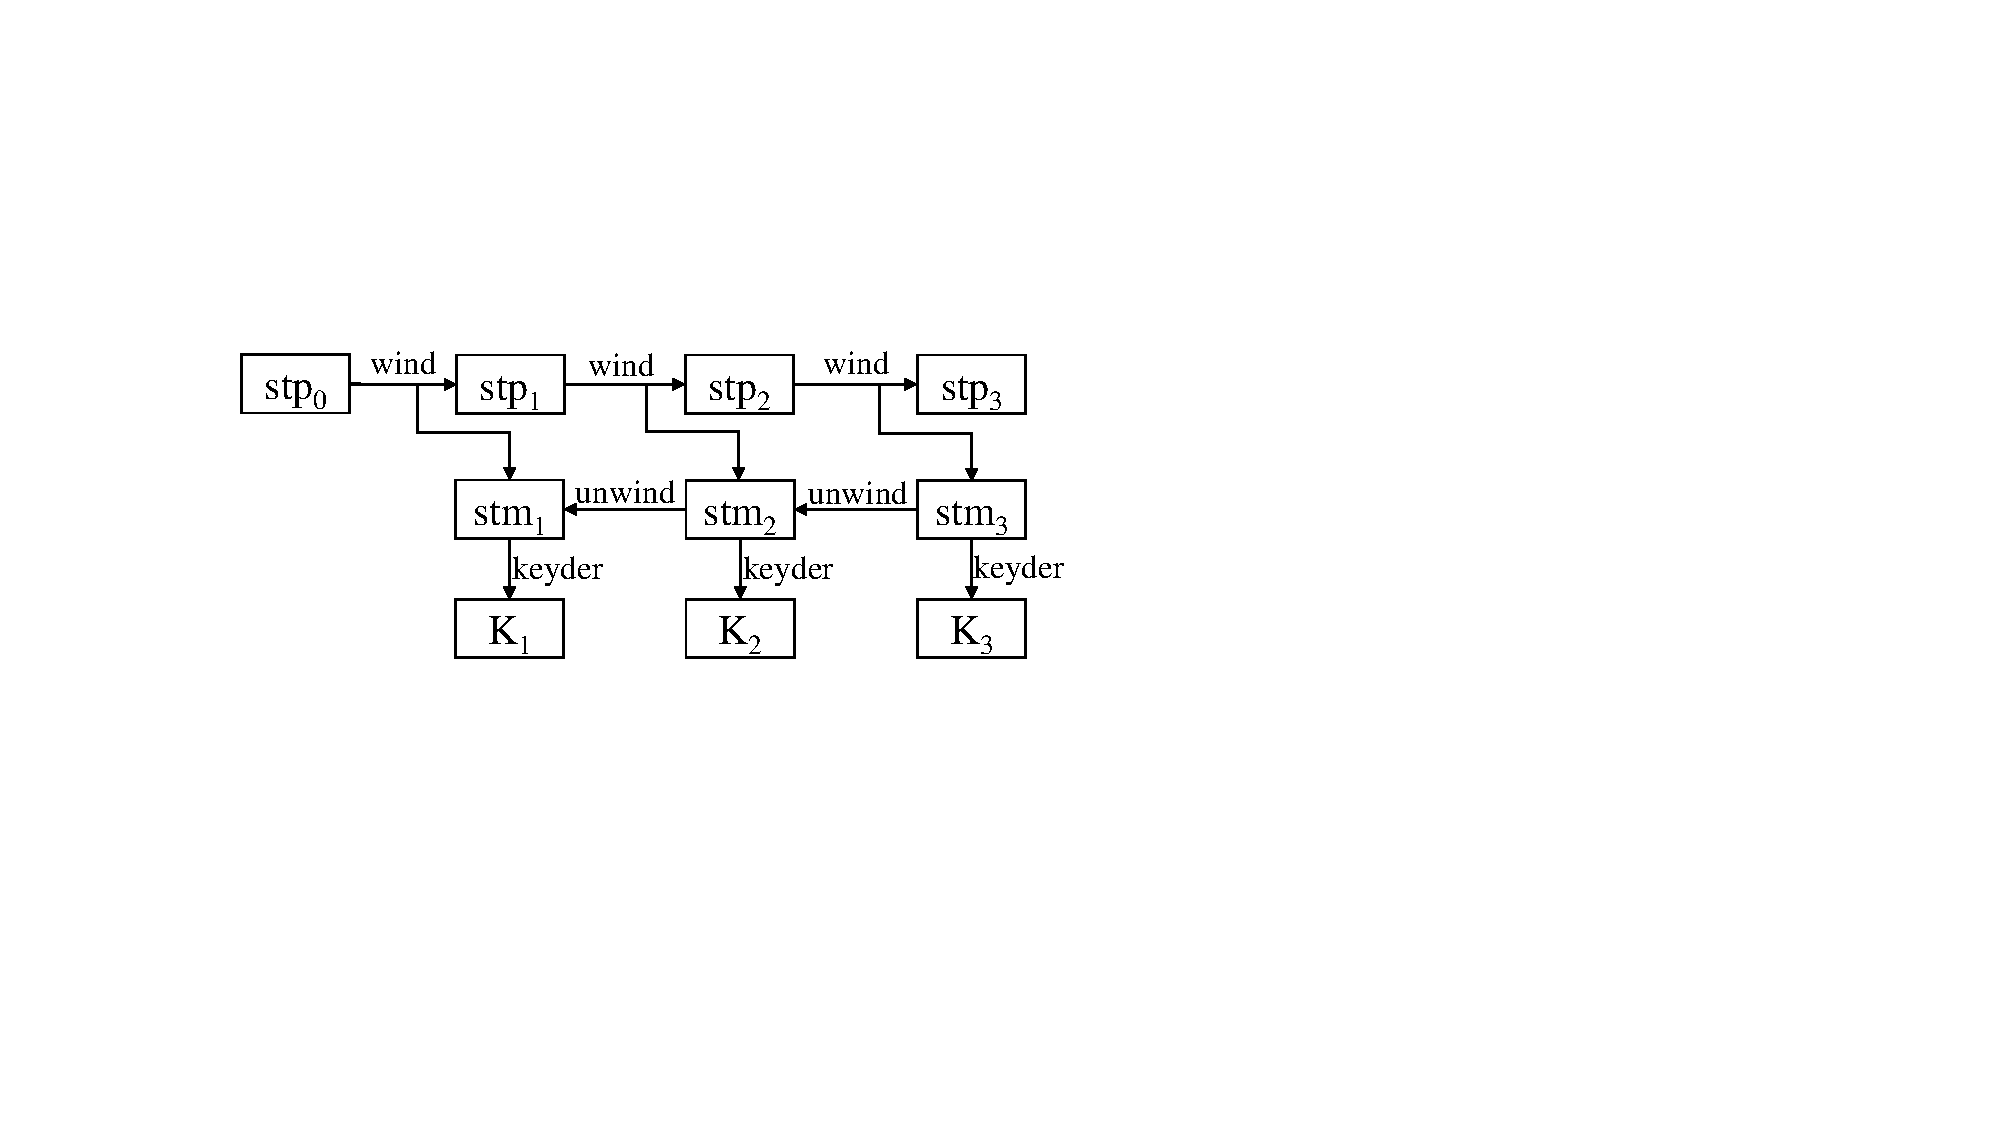
\includegraphics[width = 0.7\linewidth]{pic/密钥回归图.pdf}  
%     \caption{密钥回归框架视图} 
%     \label{密钥回归框架视图}  
% \end{figure}

密钥回归技术框架中,内容发布者并不是直接给新成员密钥$K_i$,而是给他一个成员状态值$stm_i$。新成员可以使用$keyder$函数从这个成员状态值$stm_i$推导出第$i$时间周期的密钥$K_i$。同样地,新成员也可以使用$unwind$函数从成员状态值$stm_i$推导出在此时间周期之前的旧成员状态值$stm_j$,其中$j<i$。所以,给定一个成员状态值$stm_i$,任何成员都可以推导出此时间周期及之前的密钥$K_j$,其中$j<=i$。此外,内容发布者可以使用$wind$函数将发布者状态值$stp_i$迭代生成往后的新的状态值$stp_m$,其中$m>i$,那么内容发布者的新状态值可以推导出新的密钥$K_{m+1}$及新状态前的任何一个周期的密钥,但状态值$stp_i$只能推导出周期$i+1$及之前周期的密钥。也就是说,任何状态值下的内容发布者,只有授予了成员新的状态值,该成员才有资格推导出密钥并有权解密服务器上的资源;反之,若没有被授予新状态值,则无法解密新发布的资源。

本论文支持懒惰更新的动态访问控制技术整体流程框架见图\ref{懒惰更新的动态访问控制技术流程视图},技术细节如下。

\begin{figure}[htbp]  %将服务端改成边缘存储或云存储
    \centering
    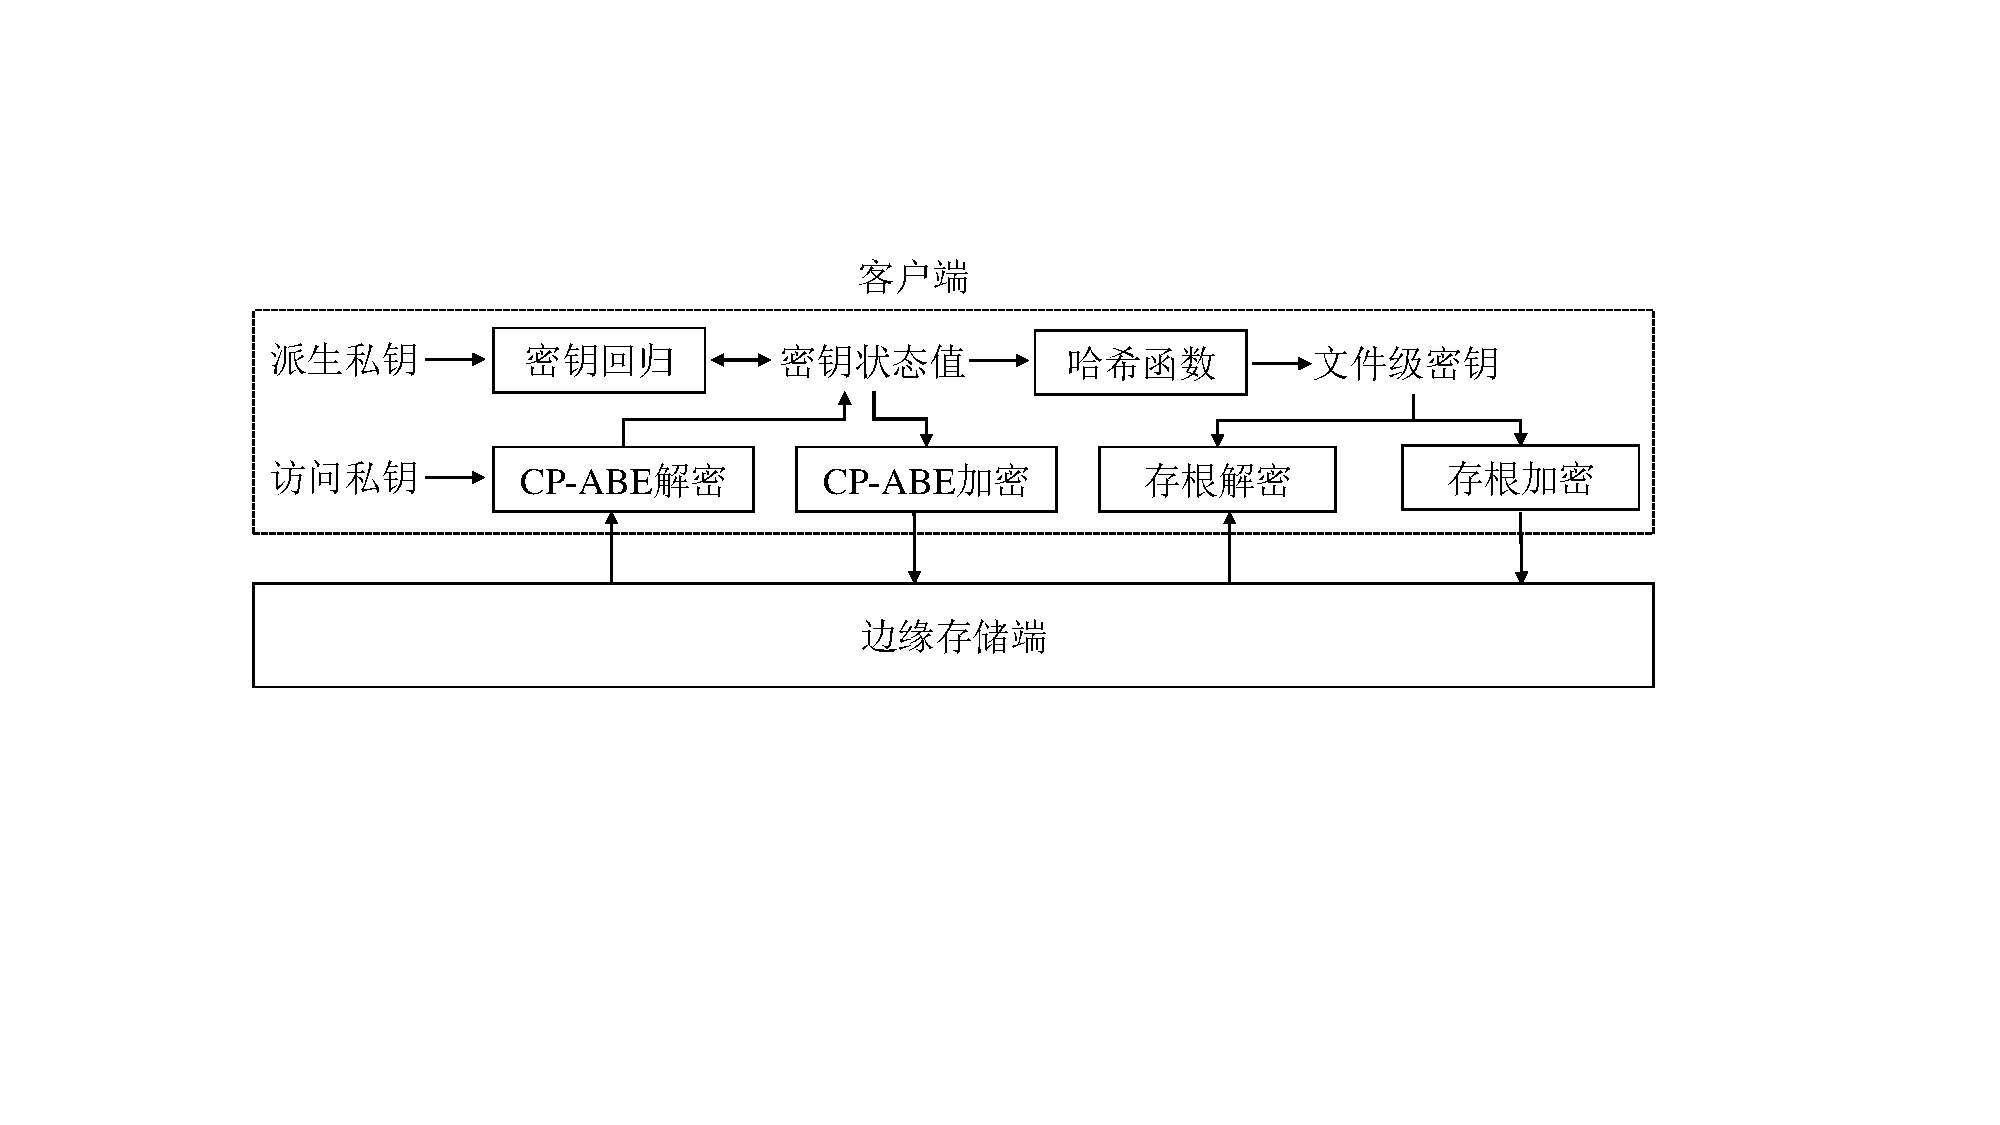
\includegraphics[width = 1.0\linewidth]{pic/dongtaifangwenkonzhi.pdf}
    \caption{懒惰更新的动态访问控制技术流程视图}
    \label{懒惰更新的动态访问控制技术流程视图}
\end{figure}

(1)访问控制。在基于密文策略的属性基加密中,每一个策略是用访问树(access tree)的形式展示的。在访问树中,每个非叶子节点都代表着一个布尔逻辑门(例如,逻辑与或者逻辑或),每一个叶子节点代表着使用者定义或规划的属性(例如,用户的所属的部门、用户员工职级、合同期限等)。每一个用户拥有和属性集合相关的私钥,如果一个用户能满足访问树的属性要求,那么他的私钥能解密密文(核心思想参考\ref{属性基加密})。简单地设计思路是,将每一个属性视为每个用户特有的唯一标识符,给每个用户一个与该唯一标识符相关的CP-ABE的私钥,称为访问私钥(private access key),并将每一个文件定义为一个所有授权用户标识符的逻辑或门的访问树,也就是说所有的授权用户都可以访问密文,其中这个密文是文件级密钥的被加密后的结果。当然,可以定义更多的属性和更复杂的访问树结构来保障更好的访问控制,在核心技术章节省略之,如有必要会在系统实现部分详细讲解。

(2)密钥更新。在懒惰更新上,本系统基于密钥回归技术(一种用于生成不同版本密钥的串行密钥推导方案,详细参考\ref{密钥回归})。简单来说,密钥回归技术引入一系列的密钥状态值,当前密钥状态值能够推导出之前的密钥状态值,但是不能推导出之后的密钥状态值。因此一个授权用户能够访问所有的之前的密钥状态值并通过密钥状态值推导出密钥解密相关的密文。与此同时,一个没有授予当前密钥状态值的(撤销权限的)不能访问任何当前及之后被新密钥保护的密文。由于能允许一个授权用户通过之前的密钥状态值访问还不是最新的密文,密钥回归技术是为了懒惰撤销而设计的,也就是说,数据拥有者可以选择在下一次更新数据的时候重加密文件。这样这些被撤销权限用户在下一次数据更新之前是允许访问当前的旧数据的,只有之后数据被更新时,这些撤销权限的用户就无法用旧密钥状态值来访问新数据了。

本系统采用基于RSA的密钥回归技术\citing{fu2006key}来解决懒惰更新问题。给每个用户分配一个唯一的公私密钥对,称为派生密钥对(derivation keys),其中派生私钥被数据拥有者用来为数据生成新的密钥状态值,而派生公钥用来推导之前的密钥状态值。对当前的密钥状态值运用哈希函数提取的哈希值作为新文件级密钥。当前的密钥状态值又和一个新的策略(new policy)关联起来,这个新策略可能是增加了新用户的访问权限而取消了些旧用户的访问权限,再采用这个新策略的CP-ABE对当前的文件级密钥加密。此时,系统只是更新了文件级密钥还没有对文件数据块的stub部分进行重加密(所以被称为懒惰更新),只有当拥有新访问权限的用户要访问数据时,会通过访问树的策略限制并用上文所说CP-ABE的访问私钥(private access key)解密获取当前最新的密钥状态值,用哈希函数提取其哈希值作为新的文件级密钥,用这个新文件密钥去重加密所有数据块的stub部分,以此实现推迟更新。由于新的密钥状态值是被新策略(例如,一个新授权策略)的CP-ABE加密保护的,那么被撤销权限的用户就不能通过CP-ABE的新策略控制,只能获取被撤销权限时刻及之前的密钥状态;而新授权的用户可以获取新的密钥状态从而获取文件的所有更新信息记录等,所以整个懒惰更新的动态访问控制技术具有很好的前向安全性(forward sercurity)。此外,系统在更新文件级密钥的时候没有立即主动用新文件级密钥重加密数据块的stub部分(主动更新),而是在新授权用户访问数据时才被动重加密(懒惰更新),这样在更新延迟方面可以节约相当的延迟时间。

(3)动态性。在(2)中着重交代了懒惰权限撤销的密钥更新的关键点在于使用密钥回归技术进行密钥状态值迭代并在新授权访问数据时才用新文件级密钥重加密数据块的stub部分。其实,密钥状态值对密钥状态值迭代并采用新策略的CP-ABE技术加密保护新密钥状态值体现了访问权限变换的动态性。换句话说,更新文件的新访问权限必然需要更新文件密钥及重加密文件的所有stub,这样被撤销权限的用户才不能完全解密密文(起码不能解密被重加密的stub部分)因而不能恢复密文的全部信息。本系统依靠着密钥回归技术的密钥状态值的迭代和赋予CP-ABE的新策略实现了动态性。

\subsection{适配“云边协同”架构}\label{适配“云边协同”架构}
上面几个小节专注于安全高效的密文去重技术本身而没有提及对“云边协同”的系统架构的适配性,本章节会对这方面加重笔墨。在探讨对“云边协同”系统的适配性之前,先简单交代一下该系统的全貌:将用户按照来源分为不同边缘服务器下的用户,不同的边缘服务器会和一个中心化的云服务进行交互相关有用信息。边缘服务器对于用户来说,既是服务提供者又是边缘缓存;云服务器对于边缘服务器来说,主要功能是数据块备份存储,即云服务不直接面向用户。此处,边缘服务和边缘服务之间并不存在安全的通信信道,那么他们的协同交互全部由云服务作为中介间接完成。

上文已经阐述过客户端将文件切分为若干数据块,每一个数据块又被加密生成修剪包(trimmed package)和存根(stub)部分。此时客户端将用文件级密钥加密一个文件所有的存根部分然后和修剪包一起上传至边缘服务器。边缘服务器会先用所有修剪包的哈希值拼接再哈希计算出一个总指纹(fingerprint)。倘若边缘服务元数据表(元数据表由文件总指纹值和文件存放位置构成)中已经存有该总指纹值,那么说明同一个文件之前被上传过,那么边缘服务器就不会存储这些修剪包,而只会存放存根和文件的元数据信息表(文件的元数据信息表存放着文件的密文数据块组成信息,密文数据块的修剪包和存根组成信息);否则,边缘服务器顺序存储这些修剪包、存根以及该文件的元数据信息,并将该总指纹值追加到服务器元数据表中。此处,边缘服务器顺序存储的优势在于机械硬盘的顺序读写性能远远高于随机读写性能因而增大了读写吞吐量。

边缘服务器会将修剪包上传至云服务器而不会上传存根部分,原因在于:\ding{172}修剪包部分是数据块的大部分支持去重,上传至云服务支持全局去重;\ding{173}存根部分只是数据块的一小部分且被用户文件级密钥加密,而每个用户选用的文件级密钥不尽相同所以存根部分并不支持去重,倘若上传至云服务会导致冗余数据降低存储效能;\ding{174}用户会更新文件级密钥而重新加密存根部分,倘若将存根也备份在云服务器上则增加数据覆盖写的次数。当边缘服务器上传修剪包至云服务器时,云服务器会根据修剪包的指纹值检索全局元数据表(全局元数据表由修剪包的指纹值修剪包存放的位置信息构成)。若命中说明之前被存储过;否则存储该数据包,并更新全局元数据表。

用户更新文件密钥时,只需将边缘服务器上的存根部分下载来重加密并上传至边缘服务器即可。此外,客户端下载目标文件时,若文件来源于本边缘服务器,则所有数据全从本边缘获取;倘若来源于其他边缘服务器,云服务则向指定边缘服务申请目标文件的元数据信息表和存根部分,然后从云后台存储上获取文件元数据中包含的所有修剪包一并发送给指定客户端所在的边缘服务器,再由边缘服务器发送给客户端。

\section{支持关联性推荐的密文检索技术}\label{keyword_search}
在阐述密文检索功能之前,先交代本系统的密文关键词检索功能不是为了达到传统意义上对称可搜索加密的安全性而设计的,而是为了海量数据的高效检索而设计的、“尽可能安全”的技术方案。该章节会对密文检索功能做出详细阐述,会对基本密文检索方案和增强密文检索做出详细交代和对比。其中,基本密文检索方案效率高而安全性稍低,所以本章节又对安全性增强的方案进行了探讨,即给出了作者的关于提高安全性的两点优化和思路分析,但没给出具体技术方案,以供后来者多墨。
\subsection{基础密文检索方案}\label{基础密文检索方案}
在\ref{系统架构}章节中,已经交代了密文关键词检索的基本流程。但在实现密文检索功能之前,每个边缘服务器还需要向中心云服务申请全局唯一的单向且抗碰撞的哈希函数,并将该哈希函数分发边缘服务下的每一个被授权的客户端。换句话来说,只有授权的客户端才有资格获取该哈希函数,才有资格用该全局的哈希函数生成关键词密文对服务器上资源检索。

客户端在上传密文文件时,会对文件明文做关键词切分,维持一个文件包含所有关键词的表备用,称为关键词备案表。并根据以下公式\citing{wang2011enabling}计算关键词和文件的关联度初始值。此处,不得不说明的是,现有文献记录的关键词和文件关联度计算公式很多\citing{wang2011enabling},本论文选用该公式原因在于该公式更简单且被众多文献所引用。其中$F_d$代表着某一个文件,$|F_d|$代表着文件的长度,$KW$代表要检索的关键词,$f_{d,KW}$代表着文件$F_d$中包含的关键词$KW$的个数。简单来说,公式\ref{关键词-文件关联度公式}体现了关键词和文件的关联度和文件长度成反比,和该文件中包含某关键词的频率呈正相关。

\begin{equation}
    Correlation(KW, F_d) = \frac{1}{|F_d|} \cdot (1\,+\,\ln{f_{d,KW}})
    \label{关键词-文件关联度公式}
\end{equation}

然后用公式\ref{关键词-关键词关联度公式}计算不同关键词之间关联度初始值,其中$F_d$代表着某一个文件,$|F_d|$代表着文件的长度,$KW_i$代表某一关键词,$Freq(KW_i, kw_j)$代表着文件中关键词$KW_i$和$KW_j$成对出现且距离小于等于指定参数$len$的频率。具体来说,公式\ref{关键词-关键词关联度公式}体现了关键词与关键词之间关联度与文件长度呈反比,与关键词成对出现频率呈正相关。

\begin{equation}
    Correlation(KW_i, KW_j) = \frac{1}{|F_d|} \cdot (1\,+\,\ln{Freq(KW_i, KW_j)})
    \label{关键词-关键词关联度公式}
\end{equation}

最后,客户端用服务器授与的全局哈希函数对关键词和文件标识符做运算隐藏真实信息,由于该哈希函数具有抗碰撞性,所以盲化后的密文关键词和文件标识符还是具备唯一性的,并用密文标识代替明文标识在网络上传输以求一定的安全性。

此外,用户端还需要构造两类主要的数据结构来维护一些重要的关联信息。其一是从关键词密文标识符到文件密文标识符的倒排索引,这也是经常被用在全文检索功能中的一个数据结构\citing{singhal2001modern};其二是关键词和关键词之间的无向图。下面,我们一一分析这些数据结构以及其保留的重要信息。

(1)关键词和文件标识符关联的倒排索引。倒排索引是一个key值为关键词,value值是一系列由文件标识和该文件与key值之间关联度组成的pair对。除了关联信息值是明文以外,关键词和文件标识符都被全局的哈希函数掩盖,所以服务器只能从倒排索引表中看出掩盖后的关键词和文件的关联强度,在基础方案中,这是不可避免的,在增强方案的思路探讨中用现有的一些密码学原语加以掩盖。倒排索引中文件的标识集合可以用堆,红黑树等数据结构表示出来,但必须严格按照关联度(correlation)排序。倒排索引被用户端提取出来后会发送至边缘服务端进行保存,边缘服务器会收集边缘下的所有授权用户的倒排索引信息,维持一张边缘下的全局表。
% \begin{figure}[htbp]  %删除图 文字描述
%     \centering  
%     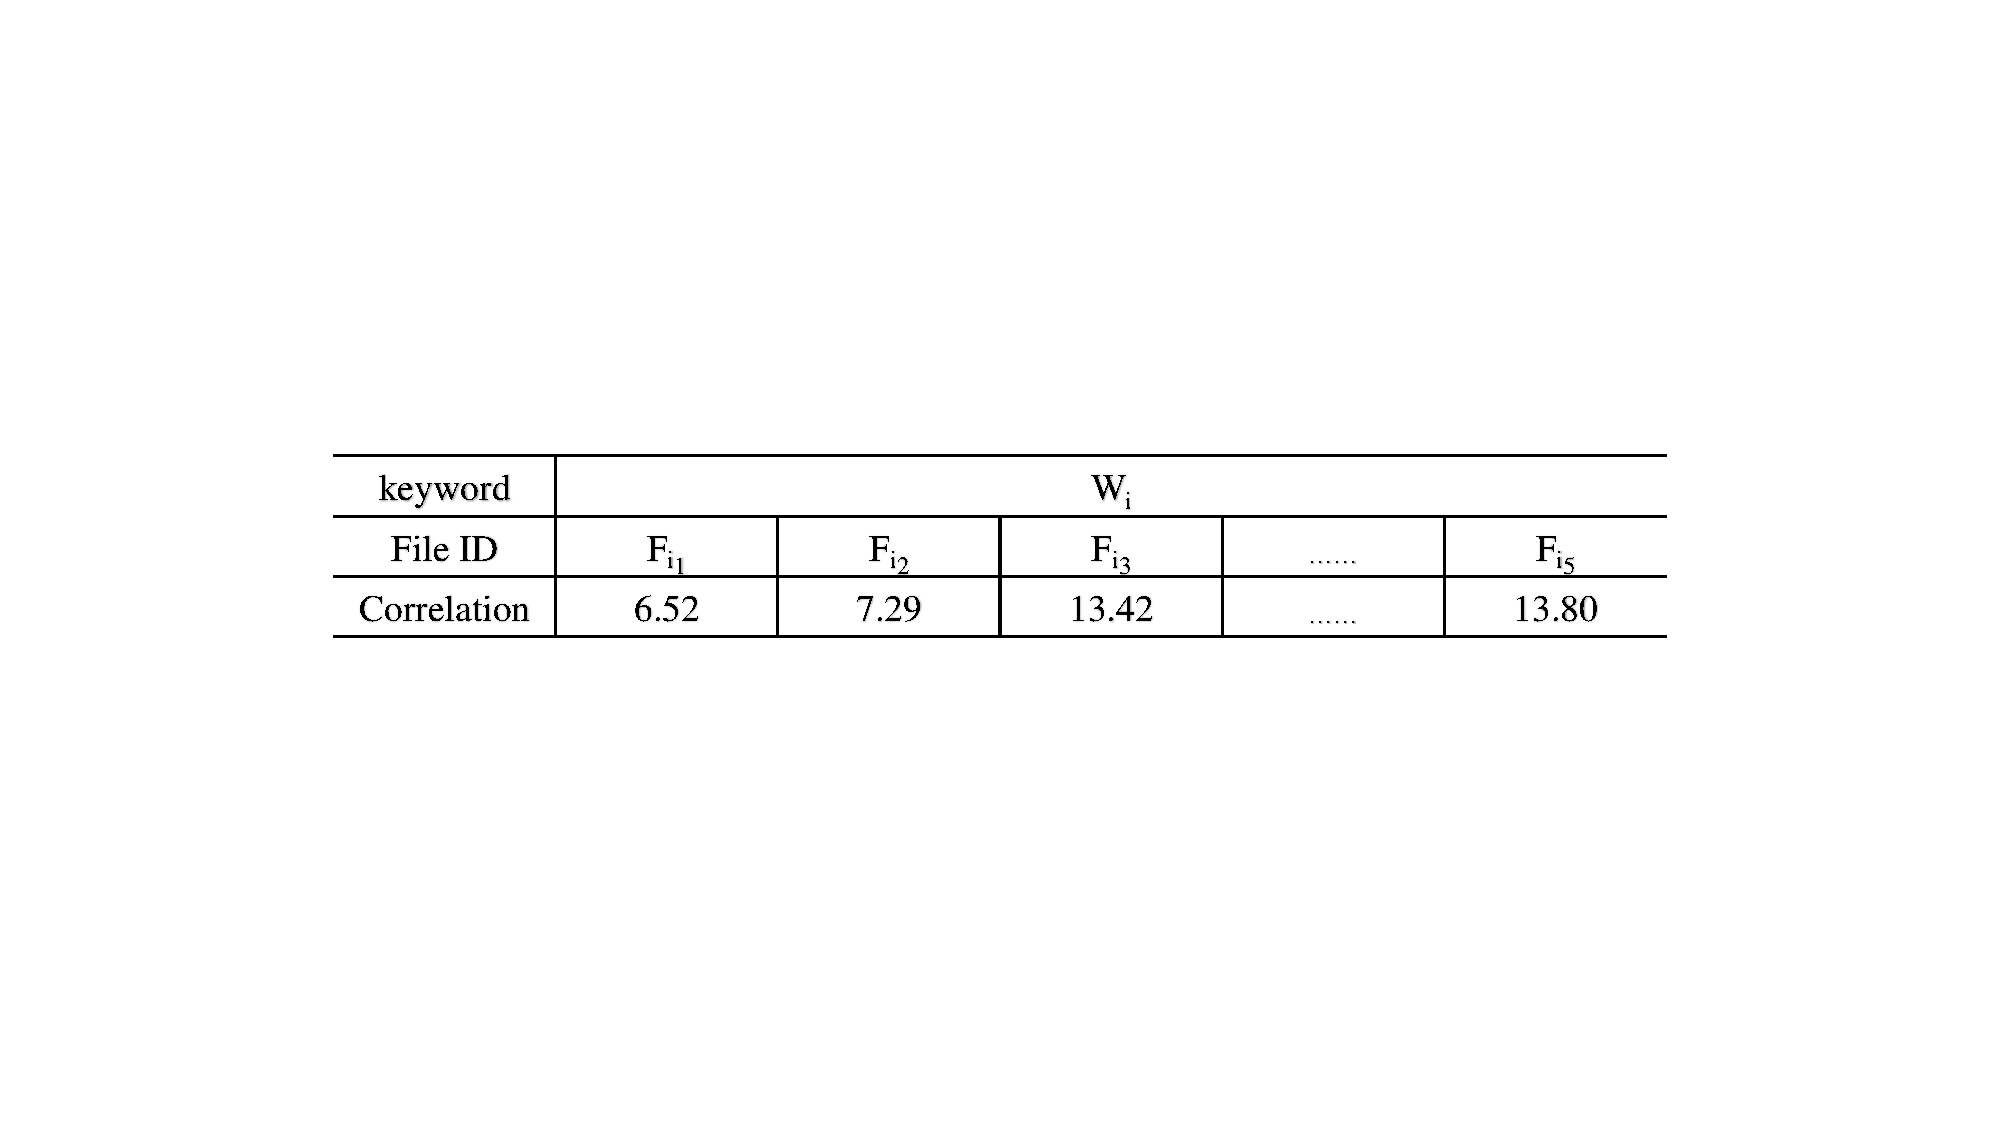
\includegraphics[width = 1.0\linewidth]{pic/倒排索引示例图.pdf}  
%     \caption{倒排索引示例图} 
%     \label{倒排索引示例图}  
% \end{figure}

当有新授权用户检索某一关键词时(先不考虑边缘服务向云服务询问其他边缘服务上的关联信息),边缘服务会根据该倒排索引表挑选关联度最高的$t_1$文件标识符返回优先返回给用户,底层逻辑在于关联度越高的文件越有可能被用户检索\citing{wang2011enabling}。但例外的情况是,用户确实向检索一项关联度更小的某一项文件。那么按照用户的翻页请求,边缘服务会依次返回按照关联度排序的文件标识符直到命中,当用户将选中的文件标识符发送给边缘服务时,边缘服务器会在密文关键词和命中文件标识符的关联度值增加权重$w$并更新倒排索引相关的条目保证包含该关键词的文件标识符依旧保持着关联度的有序性。这个权值$w$是值得周密设计的,倘若前面用户的检索行为更影响后面用户行为,那么不妨稍微加大这个权值$w$。换句话来说,往往一个热点文件会常常被检索,所以前面的用户行为启发式地增加权值,以便后面检索用户在更短的时间内获取目标文件。当然,这里涉及的推荐算法,本系统不做过多的探讨和设计,以待后面研究者加大笔墨。
当考虑边缘服务向云服务询问其他边缘服务上关联信息时,图\ref{密文检索流程图}中交代了全局服务器的全局询问流程:全局服务器会向其他各边缘服务器请求执行相同的密文关键词检索功能。此处,本系统只设计了最关联的前$k_1$项来自于其他边缘服务器的文件标识符。根据局部性原理,同一边缘服务下的用户检索同一边缘服务器上的资源倾向更高。当然,例外的情况时有发生,所以本系统会随着不命中次数增加而逐步增大$k_1$值,维护一个步长$step_1$。步长$step_1$具体值是个值得深究的话题,大抵应该和客户端展示条目数成正相关,和网络占用情况呈负相关。此处,本系统不做深究,以待后来人多关注。最后,当命中的是其他边缘服务器下的文件时,需要通过云服务器向其他边缘服务器发送特殊指令,表明需要在相应的关联度上增加权重$v$,此处$v$应该比$w$小,表明来源于其他边缘服务的检索影响比来源本边缘的更小。将上述服务端的操作整理成一个算法\ref{关键词的关联文件检索算法},如下。

在具体实现的时候,本算法还有值得优化的几个点。比如,哈希值合法且存在于倒排索引中的判断需要前置一个布隆过滤器(Bloom filter),对密文关键词的定位需要用到一些直接定位数据结构等。这些优化不是技术核心要点,会放在系统实现部分详细交代。

(2)关键词与关键词关联的无向图。如图\ref{关键词-关键词关联度示例图}所示,在图中,$KW$代表关键词(keyword),$C_{i-j}$代表第$i$和$j$关键词之间的关联度,初始化为\ref{关键词-关键词关联度公式}的计算值。同样地,关键词是被单向哈希函数所掩盖,但是关联度是明文传输给服务器。关键词间的无向图会被客户端提取出来并初始化权值发送给边缘服务器,边缘服务器会维持边缘下的全局无向图,形式结构同图\ref{关键词-关键词关联度示例图}。
\begin{figure}[htbp]
    \centering
    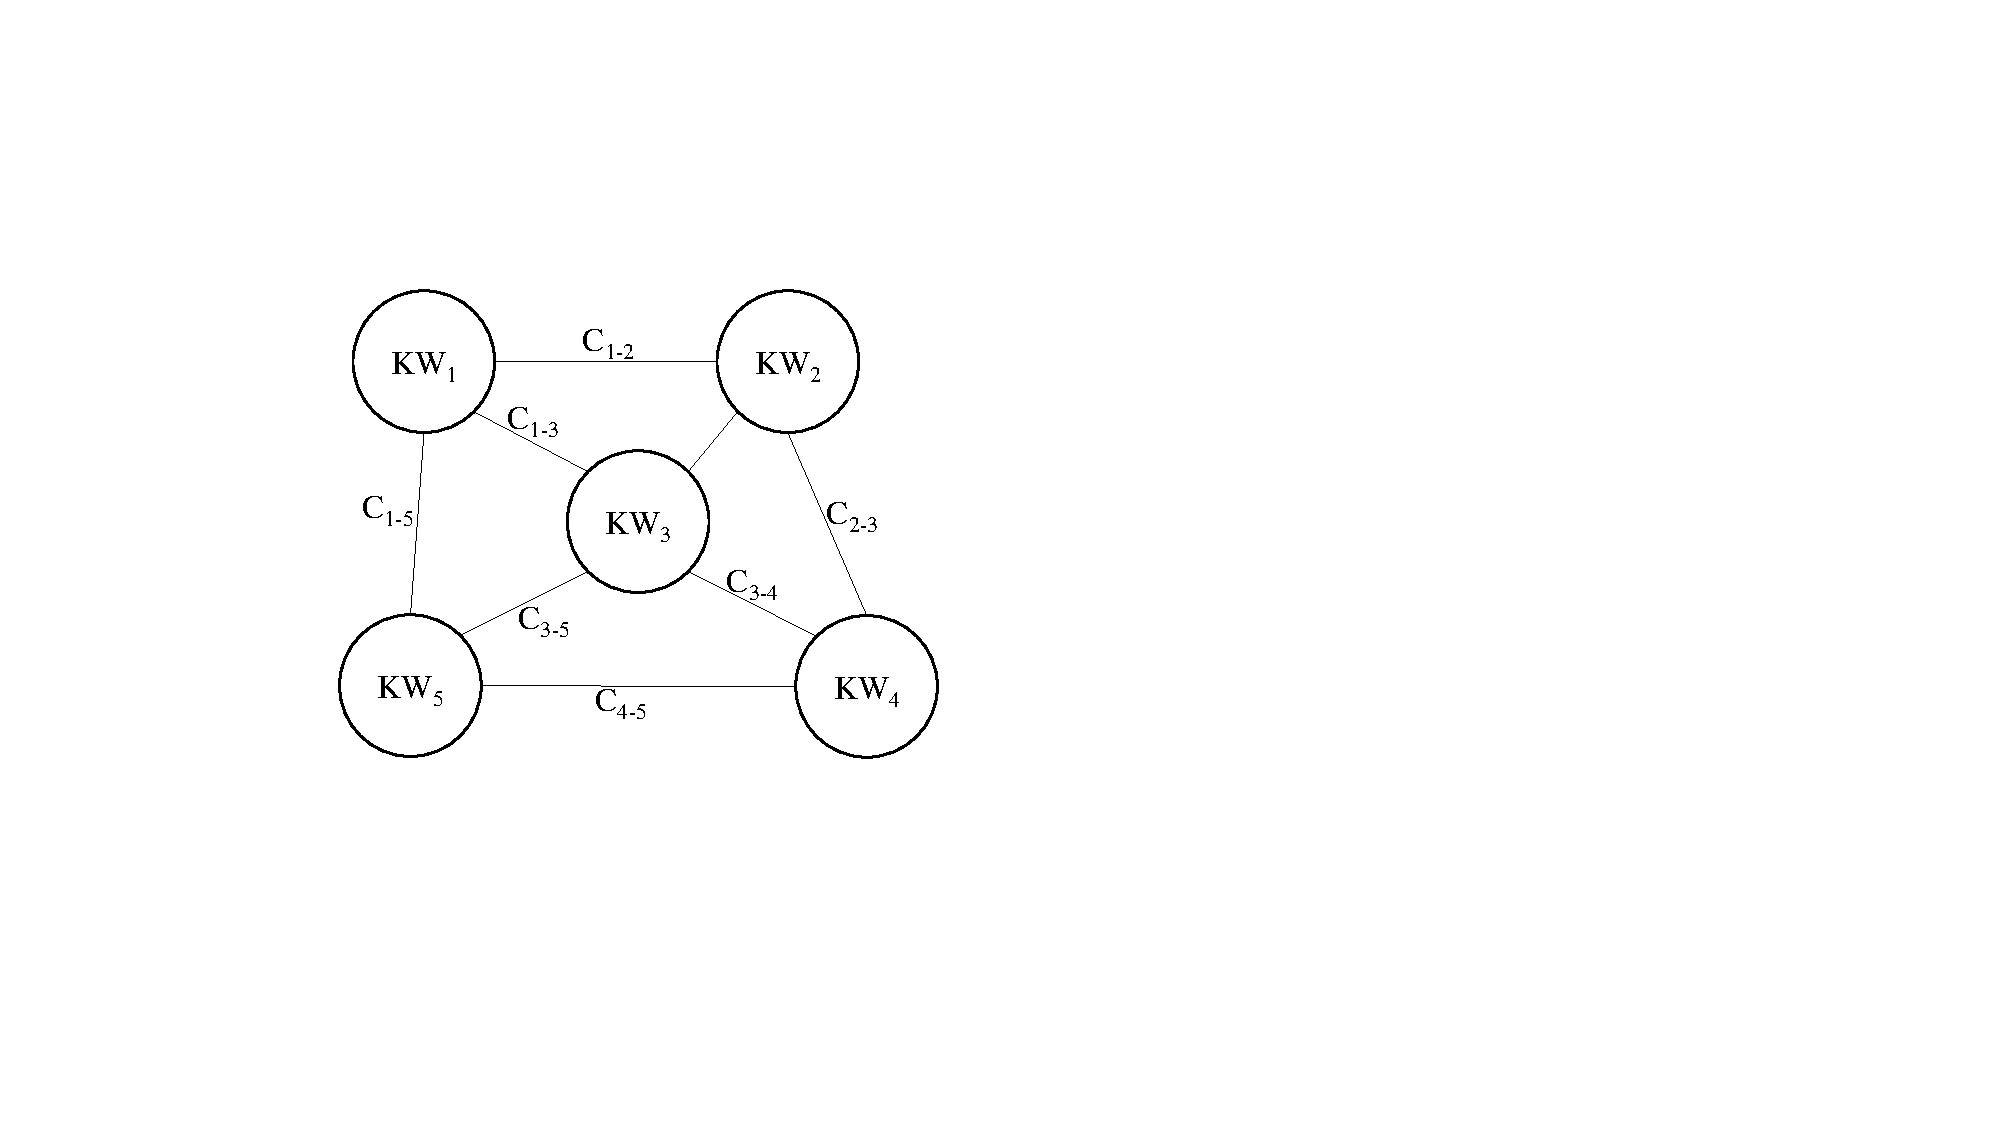
\includegraphics[width = 0.6\linewidth]{pic/关键词关联度示例图.pdf}
    \caption{关键词-关键词关联度示例图}
    \label{关键词-关键词关联度示例图}
\end{figure}

当有授权用户检索某一关键词时,边缘服务器会根据关键词-关键词无向图定位关键词所有相邻关键词以及其关联度(边权值),按照边权值从大到小逆序排列,挑选其中最相关的$t_2$项关键词,并依次对每一个关键词检索边缘服务下的关键词和文件标识符的倒排索引,并按照下公式\ref{得分公式}的计算结果进行排序,选出最大的$n$项作为密文关键词检索的推荐,若没有命中则不断扩大$n$的值。公式\ref{得分公式}中,$KW$是指关键词,$F_d$是指文件。该公式可以视为公式\ref{关键词-文件关联度公式}和公式\ref{关键词-关键词关联度公式}的线性组合,$a$和$b$视为组合系数,且$a + b = 1$,$a>0$,$b>0$。
\begin{equation}
    Score(KW_i, F_d) = a \cdot Correlation(KW_i, KW_j) + b \cdot Correlation(KW_j, F_d)
    \label{得分公式}
\end{equation}

同样地,云服务器还会咨询其他边缘服务这个关联推荐的结果整合出最大的$k_2$项。当没命中时,相应地增大选中的相关关键词数量和相邻关键词的关联关键的数量,维持一个变量步长$step_2$;命中时,按照关键词备案表(关键词备案表其实就是每一个文件的关键词关联信息的汇总信息表)找到目标文件下的所有关键词,并更新\ref{关键词-关键词关联度示例图}中的边权值。其中,若文件来自于本边缘服务器,那么边权值增加$w$;若文件来源于其他边缘服务器下,相应地的增加$v$,此处$w$和$v$和(1)中相同,此处不赘述。为了表述清楚这个流程,现将主要步骤描述在算法\ref{关键词相邻关键词的关联文件检索算法}中,算法\ref{更新小顶堆算法}很好地将算法\ref{关键词的关联文件检索算法}融入进来,通过调用每一个最相邻关键词的关联文件检索算法得到最关联文件不断更新小根堆并推送给客户端。

密文检索的关联性分析和推荐主要体现有两点:\ding{172}通过密文关键词和文件标识符建立一对一的联系,初始化其关联度并随着用户的检索行为不断更新关联度,因为关联度值启发式地影响后面读者的检索行为,这样前面读者的用户访问行为会被统计和累积并切实记录在关联度数值中,关联度数值影响着关联文件的排名,也影响着被推送给用户的次序,这种动态的变动关联度形成推荐根据是以往工作中少见的;\ding{173}本系统不仅建立密态关键词和文件的关联,还建立了密文关键词和关键词的关联,再通过关联关键词去查找关联文件,独创地提出了关键词关联度公式\ref{关键词-关键词关联度公式}和关联总分公式\ref{得分公式},并以公式\ref{关键词-关键词关联度公式}获取最相邻关键词,再以关联总分公式\ref{得分公式}计算某一关键词间接关联的总得分,以总得分为根据排序选出最大得分的若干项推荐给用户,这样的间接关联性通过两个公式量化的方式也是已有工作中鲜有的,此外前面读者的检索行为会影响关键词-关键词关联的无向图的边权值,启发式地影响后面读者的检索行为。
\SetKwInput{KwIn}{输入}
\begin{algorithm}[H]
    \KwData{边缘下全局倒排索引-$inverted\,index$}
    \KwIn{关键词的哈希值-$keyword\,hash$}
    初始化$pos = 0$\;
    \eIf{哈希值合法且能在inverted index中找到keyword hash}{
        \While{$pos$小于关联文件个数}{
            挑选关联文件(已倒叙排列)的第$pos$到$pos+t_1-1$个\;
            询问云服务其他边缘服务下关联度最高的$k_1$项文件\;
            发送给客户端,等待回应\;
            \eIf{命中}{
                \eIf{来自于本边缘}{
                    相应关联度自增$w$\;
                }{
                    相应关联度自增$v$\;
                }
                break\;
            }{
                $k_1 = k_1 + step_1$\;
                $pos = pos + t_1$\;
                $t_1 = t_1 +step_1$\;
            }
        }
    }{
        返回非法行为\;
    }
    \caption{关键词的关联文件检索算法}
    \label{关键词的关联文件检索算法}
\end{algorithm}

\SetKwInput{KwIn}{输入}
\begin{algorithm}[H]
    \KwData{边缘下全局倒排索引-$inverted\,index$,边缘下的全局关键词关联无向图-$graph$}
    \KwIn{关键词的哈希值-$keyword\, hash$}
    初始化$pos = 0$\;
    初始化一个大小为$n$的小根堆$HEAP_1$,大小为$k_2$的小根堆$HEAP_2$\;
    \eIf{哈希值合法且能在graph中找到keyword hash}{
        \While{pos小于关联关键词个数}{
            挑选关联关键词的第$pos$大到$pos+t_2-1$大\;
            调用算法\ref{更新小顶堆算法}并输入第$pos$大到$pos+t_2-1$大的关联关键词\;
            发送$HEAP_1$和$HEAP_2$中的文件标识符给客户端,等待回应\;
            \eIf{命中}{
                \eIf{来自于本边缘}{
                    根据关键词备案表对所包含关键词的相应关联度自增$w$\;
                }{
                    根据关键词备案表对所包含关键词的相应关联度相应关联度自增$v$\;
                }
                break\;
            }{
                $k_2 = k_2 + step_2$\;
                $n = n + step2$\;
                $pos = pos + t_2$\;
                $t_2 = t_2 +step_2$\;
            }
        }
    }{
        返回非法行为\;
    }
    \caption{关键词相邻关键词的关联文件检索算法}
    \label{关键词相邻关键词的关联文件检索算法}
\end{algorithm}

\SetKwInput{KwIn}{输入}
\begin{algorithm}[H]
    \KwData{边缘下全局倒排索引-$inverted\,index$,边缘下的全局关键词关联无向图-$graph$}
    \KwIn{第$i$到第$j$个相邻关键词}
    \While{第$i$到第$j$个相邻关键词}{
        执行算法\ref{关键词的关联文件检索算法}得到$t_1$项本边缘下的结果,$k_1$项其他边缘下的结果\;
        分别用公式\ref{得分公式}计算得分并丢进$HEAP_1$和$HEAP_2$\;
    }
    \caption{更新小顶堆算法}
    \label{更新小顶堆算法}
\end{algorithm}

\subsection{安全性增强方案探讨}\label{安全性增强方案}
在基础密文检索方案(见\ref{基础密文检索方案})中,探讨了兼具关联性分析和推荐功能的密文检索功能的详细技术细节,其中包括了关键词-文件的关联度、关键词-关键词关联度更新的细节和整个关联系分析和推荐的算法流程。基础密文检索方案简单且高效,似乎已经是完美的了,但其实依然存在不足:为了对关联度值动态更新,不得不将关联度值设置成明文存储在服务端,给予服务端窥探关键词密文和文件标识符密文之间的关联度的机会,存在潜在威胁。

为了规避潜在的风险,将关联度值也设置成密文是一个不错的方法。但如果将关联度值设置成密文,则无法像对明文做更新操作那般简单操作关联度密文值。于是,在本章节进行一些安全性增强方案的启发式探讨,也就是说,本章节并没有给出具体的安全性增强方案技术细节,而是给出了一些安全性增强的思路来优化基础方案。在探讨安全性增强的思路前先交代两种加密原语。

\textbf{同态加密}\label{同态加密}

同态加密(Homomorphic Encryption,HE)是指满足密态同态运算性质的加密算法,也就是说数据经过同态加密之后对密文进行特定的计算后再进行同态解密得到的明文结果,和对原始明文进行同样计算的结果完全一致,实现数据的“可算不可见”,同态计算的性质如下图\ref{同态加密性质}所示。
\begin{figure}[htbp]
    \centering
    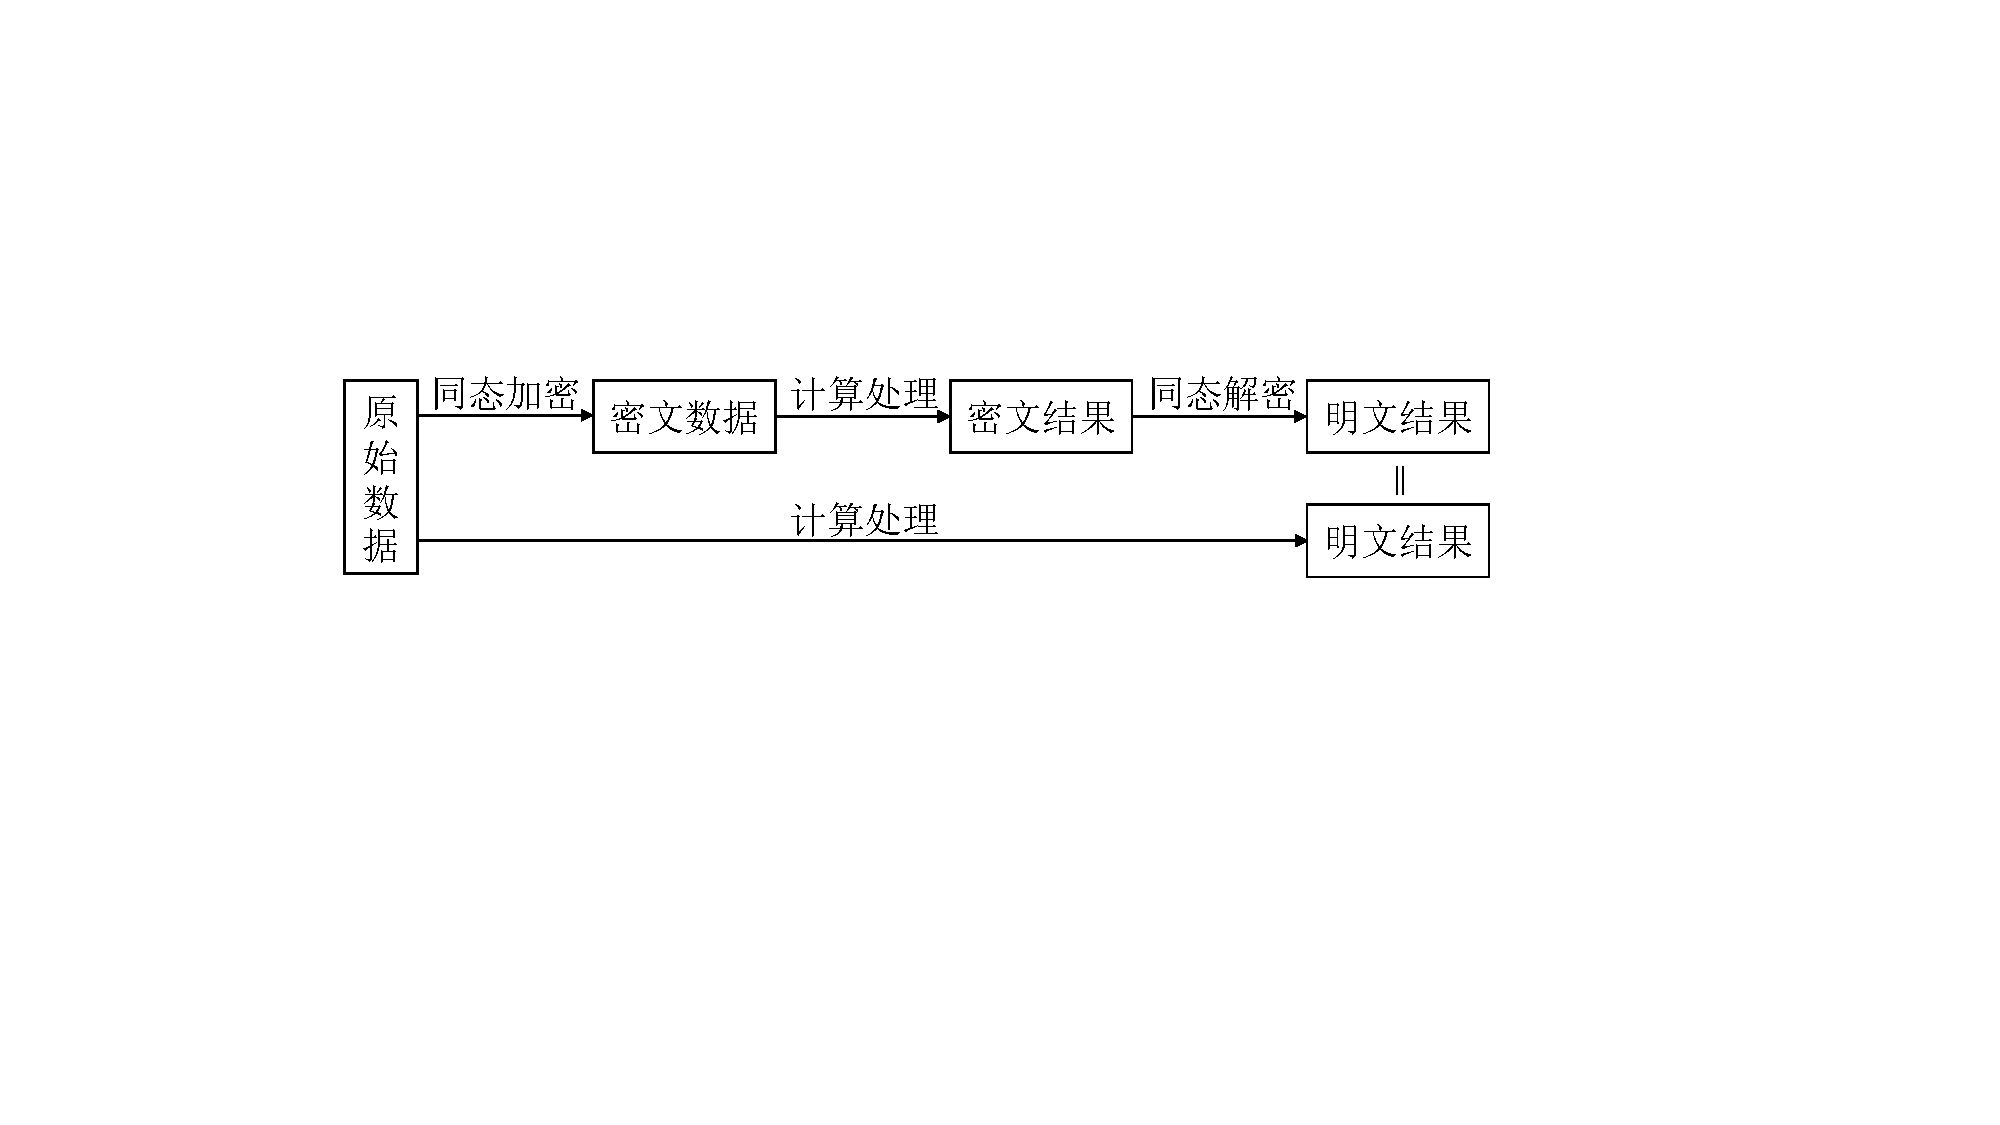
\includegraphics[width = 0.8\linewidth]{pic/同态加密性质.pdf}
    \caption{同态加密性质}
    \label{同态加密性质}
\end{figure}

同态加密目前已有的研究将其划分为全同态加密和半同态加密,半同态加密有时候也被称为部分同态加密。全同态加密是指支持对密文进行任何形式的运算;半同态加密是指仅支持部分形式的运算,例如仅支持加法、乘法或有限次的加法和乘法运算。目前,同态加密算法在很多领域都有落地应用\citing{acar2018survey},其中包括区块链、联邦学习和云计算等涉及隐私计算需求的场景。其中全同态加密算法仍处于探索和研究阶段,现有的一些算法存在着诸多不足:运行效率低、密钥过大和密文爆炸等,在效率和性能方面和可行过程应用还存在一定的差距;半同态在现实场景应用较多,比如加法同态加密。


\textbf{保序加密}\label{保序加密}

保序加密(Order-Preserving Encryption,OPE)是一种保留原始明文顺序的加密方案,也就是说,倘若原始明文有大小顺序,那么保序加密之后还能保证这样的顺序,它能在保护用户数据隐私的前提下实现密态范围查询的功能。当客户端进行范围查询时,客户端只要给服务端传输区间两个端点的的密文,然后服务端根据已有顺序的密文数据并对照两个端点值查找区间内的所有符合要求的数据。最后,服务端返回符合要求的数据给客户端。通俗来说,客户端允许服务端知道明文的顺序信息而不允许服务端知道明文的具体值以及其他信息。

现有的一些保序加密方案可以按照其构建过程是否存在索引分为无索引结构的保序加密方案和基于索引结构的保序加密方案。其中,无索引结构的保序加密是指加密密文保留了明文的顺序信息;基于索引结构的保序加密方案是指通过一般的加密方案(例如AES、DES)对明文数据进行加密,同时建立一个安全的保序索引结构,用于存储明文顺序信息。因为其保留明文顺序信息的特性,保序加密方案常常被应用在排序的密文关键词检索方案中。在本系统的密文检索方案中,安全性增强的密文检索方案的一个思路就是利用安全可信的第三方对明文进行保序加密并委托给服务端,服务端根据保留的明文顺序信息进行关联度的分析和推荐。

客户端对明文的关键词切分、提取关键词和文件标识符的哈希值以及计算关键词-文件关联度和关键词-关键词关联度的初始值和基础密文检索方案中完全一直。不同的地方在于:客户端利用同态加密对关联度初始值加密并发送给服务端。由于同态加密原语的密文同态运算性质,服务端对关联度的计算是“可算不可见”的(同态加密的描述见\ref{同态加密})。服务端对关联度密文更新后,客户端解密密文得到的明文也是被更新的,换句话来说,服务器对关联度密文的更新能被一一映射在明文的更新中。但这会带来一个严峻的问题:服务器在不得知关联度数值明文的前提下无法按照关联度数值进行排序,也不能完成关联度最高的若干项分析和推荐。对于这个问题的解决,本论文提供以下两种思路:

(1)服务端只针对关键词的相邻关键词和文件进行检索,将检索到的所有关键词和文件标识符都发送给客户端,客户端解密关联度值、指定想要查询的相邻关键词或者文件标识符并发送给服务端,服务端根据客户端的指令返回对应的文件密文或根据新关键词再检索。该方案存在着效率和性能的不足,也就是说,由于多了客户端和服务端之间的两次网络通讯,并且其中有一次是服务端发送了大量的关联信息(其中包括关键词密文、文件标识符密文以及对应的关联度值,虽然只是一些很小的字段,但是由于服务端可能存在大量相邻信息,所以总量是不可忽略的),这不仅浪费了检索的时间和增大了用户检索请求的响应时间,还占用了大量的通信带宽和引发网络拥堵。此外,由于客户端的计算能力并不是很高,对大量的关联度值的解密严重浪费了宝贵且稀有的客户端计算资源。

(2)假设整个系统中存在一个可信的、计算能力比客户端强的第三方,称为保序加密管理器,它负责接受来自服务器的关联信息,并对其中的关联度解密成明文,然后按照明文值的大小进行保序加密(保序加密的描述详见\ref{保序加密}),详细地说,按照明文大小顺序建立索引,索引的指针应当指向关键词的密文或者文件标识符的密文。这就在不透露任何明文信息的前提下告诉服务器关联度值的排序信息,那么服务器便可以按照排序信息接着向客户端进行最关联的若干项推荐。不命中的话增多推荐项;命中的话更新关联度值的同态加密之后的结果。后续步骤基本和基础密文检索方案中完全一致。该思路解决了思路(1)中客户端计算能力不足的问题,但是仍然存在两次通信的问题。此外,本论文假设的保序加密管理器理想化,在工程中难以实现;新增一个加密过程,即保序加密,也会加重算法复杂度和响应延迟高的情况。

当然,增强方案的思路也是存在着不足的:比基础方案涉及的加解密过程多了至少一次(思路1涉及同态加解密,思路2涉及同态加解密和保序加解密)、通讯过程多了两次,所以效率较低,并且对用户密文检索的响应延迟很高。



\subsection{适配密文去重系统}
本论文的密文去重系统是基于“云边协同”架构的,所以对于密文去重系统的适配性必须涉及两个方面:对“云边协同”架构的适配和对密文去重技术的适配。

在适配“云边协同”架构方面,在基础密文检索方案(见\ref{基础密文检索方案})中,交代了云服务作为密文检索流程中的中间人地位:对其他边缘服务下文件关联性咨询都是由云服务发起的。当用户检索到目标文件并需要下载该文件时,倘若该文件来源于其他边缘服务,则云服务向该边缘服务索要文件的元数据信息表和存根部分,并从云服务后台存储恢复文件的修改包部分一起发送给客户端所在的边缘服务器,再由边缘服务器发送给客户端(见\ref{适配“云边协同”架构})。

在适配密文去重技术方面,主要是检索功能和权限校验的适配。具体来说,本论文的检索功能基于全局唯一的哈希函数生成的关键词哈希值,每一个合法用户都有权限去检索关键词关联文件,但是解密文件需要通过CP-ABE的策略控制,所以合法用户能检索到文件的唯一标识符,但是并不一定能解密甚至查看文件的内容。当某用户不能解密和查看文件内容时,如有必要,可以向文件主申请权限,文件主会更新控制访问的策略从而授权该用户。
\section{安全性分析}
本系统主要涉及两个核心技术点:兼容密钥更新的安全高效密文去重技术和兼容关联分析的密文检索技术,其中密文去重技术又可以细分为基于CAONT的密文去重技术和基于相似性的密钥生成技术两个部分。为了展示完整了安全性分析逻辑,本章节先论证基于CAONT的密文去重技术的机密性和完整性,再在此基础上论述基于相似性的生成密钥的安全性,最后阐述密文检索技术的安全性分析。

基于CAONT的密文去重技术的安全性分析分为两个部分:数据机密性和完整性。

对于数据机密性(confidentiality )而言,主要有三个层次。首先,对手可以从受损的服务器访问所有经过修整的包、加密的存根和加密的密钥状态。由于对手无法泄露任何私有访问密钥(private access key)和私有派生密钥(private derivation key),因此无法恢复所有修剪的包和加密存根。因此,本系统实现了与DupLESS相同的保密级别。其次,对手可以与被撤销或未经授权的客户端串通,通过这些客户端,对手可以学习一组私有派生密钥和私有访问密钥。由于CP-ABE和密钥回归的保护,这些泄露的私钥不能用于解密超出其访问范围的文件密钥密文。如果没有正确的文件密钥,对手就无法推断出有关底层块的任何信息。一个特别的注意事项是,客户端可以在CAONT中保留块的MLE密钥(在基本加密中)或哈希密钥(在增强加密中),以使块即使在被撤销后也可以访问。然而,如果块被更新,则被撤销的客户端无法从更新的块中获知任何信息,因为CAONT将使用新的MLE密钥或哈希密钥来转换更新的块,从而使旧的块变得无用。最后,对手可以监视客户端的子集并识别它们请求的MLE密钥。基于CAONT的增强加密方案确保了不可预测区块的机密性,即使受害者客户端被授权访问这些区块。具体来说,增强的加密方案使用文件密钥构建了一个额外的安全层。只要文件密钥是安全的,由于CAONT的保护,恢复MLE密文(即CAONT输入)在计算上是不可行的。请注意,对手可以通过发起暴力攻击来恢复MLE密文,以检查MLE密文是否通过CAONT转换为修剪包,但如果块是不可预测的,则在计算上是不可行的。因此,识别MLE密钥无助于恢复原始块,因此原始块保持安全。

对于完整性而言,基于CAONT的基础加密方案和增强加密方案都确保了块级别的完整性,从而可以检测到对修整包或块存根的任何修改。在基础加密方案中,MLE密钥要可以通过$K_M = t \oplus H(C)$公式还原,其中$t$代表着数据包的尾巴,$C$代表着头部,$H(\cdot)$代表哈希函数。由于$H(C)$依赖于$C$的每一比特位,因此对包的任何部分的修改都会导致不正确的$K_M$。因此,客户端可以通过检查填充有还原块的“金丝雀”$c$来轻松检测篡改。使用类似的方式,增强的加密方案也确保了块的完整性。客户端通过比较$H(C_1||K_M)$是否等于$h$来执行完整性检查。关于增强方案的一个特别注意事项是,即使包被篡改,其使用自异或(self-XOR)操作也可以返回正确的哈希密钥$h$。例如,有智慧的对手可以将$C_2$分成固定大小的分片,并将这些分片的偶数号翻转相同的比特位。另一方面,即使使用了正确的哈希密钥,被篡改的包也会被恢复为错误的输入,通过将其与$h$进行比较,可以发现其违反了完整性。注意,本段中涉及的符号在基于CANOT的数据加密和密钥更新技术(见\ref{基于CANOT的数据加密和密钥更新技术})中都有相应说明。

然后,分析一下基于CAONT的基础加密和增强加密两种方案上的相似性MLE密钥生成技术的安全性。基础加密方案的相似性密钥生成技术不具备数据的机密性,原因是它使用分段级MLE密钥(源自分段的最小指纹)作为CAONT的输入,以转换段中的所有块。这将为同一段中的所有块创建相同的伪随机掩码$G(\cdot)$。这允许对手将异或操作应用于任何两个生成的修整包以移除掩码,并学习原始块的大部分异或结果。然而,密钥生成技术不会给增强加密方案带来任何安全问题,原因是伪随机掩码是从MLE密钥和MLE密文生成的。结果,不同的块导致不同的伪随机掩码,在不知道文件密钥的情况下,这些掩码是不可能被移除的。尽管基于相似度的MLE密钥生成允许对手通过请求MLE密钥获取潜在的最小指纹来缩小在线暴力攻击的攻击空间,但密钥管理器可以降低密钥生成请求的速率限制。由于段级密钥生成已经减少了密钥生成请求的数量,因此降低速率限制对正常用户没有影响。因此,增强型加密方案可以从基于相似度的MLE密钥生成中获得性能增益,并根据我们的评估实现与基本加密方案类似的性能。

最后分析一下本系统设计的密文检索技术的安全性。密文检索中对所有的关键词和文件的指纹提取都是使用的全局唯一的哈希函数,那么当敌手攻陷了某被撤销或未经授权的客户端并且由该客户端发起某些关键词检索时,敌手也只能获得包含该关键词的文件指纹信息。当敌手想要恢复明文时,由于CP-ABE和密钥回归技术的保护,敌手不能访问超出范围的文件密钥,更不能解密存根部分。此外,密文检索技术中的关联度值都是以明文形式存放于服务器上的,服务器想学习具体的关键词和文件间的关联度是无法完成的:哈希函数的单向性保证了服务器只能知道关键词和文件的指纹值而无法反推明文。当然,任何信息以明文的形式存放在服务器上都会存在一定的安全隐患,但是为了让服务器高效地更新和维护关联信息更好地进行关联分析和推荐又不得不向服务器透露关联度的明文。所以,本系统的密文检索技术做到了“尽可能安全”。

\section{本章小结}
本章节主要针对密文去重系统的两部分技术核心做了详细交代。首先交代了系统架构,介绍系统整体外观并交代了这种架构方式的优势。然后,分析威胁模型并引入本系统设计的三个安全性目标。为了达成这三个安全性目标,本论文有条理地介绍了两大核心技术点:兼容密钥更新的安全高效的密文去重技术和兼具关联性推荐的密文检索技术。在密文去重技术中,详细交代了安全和高效的突出点以及是如何兼容密钥更新的;在密文检索技术中,详细阐述关联值的公式表述和更新以及关联分析和推荐的功能实现流程。最后,在每个技术点后面都交代了对“云边协同”架构适配性,并且在密文检索技术的最后交代了两个技术点的兼容性。
\chapter{系统实现和实验评估}
本章节主要关注于整个系统实现以及实现评估,会对上一章(见\ref{系统设计和技术细节})中涉及的两个方面的技术核心思想进行实现,尤其是上一章节被忽略的系统实现细节和值得优化性能而需要新增的组件。此外,还有整个系统的安全性分析和各方面的性能评测。

\section{系统原型实现}
在本节中,不会分别讲述每一个技术点的实现而是按照客户端和云、边服务器的底层原理探究整个系统的实现。接下来,本论文会先阐述客户端实现所需要的重要组件,其次讲述边缘服务器和云服务的实现,然后简单交代密钥管理器的实现,最后阐明对整体系统的优化。
\subsection{客户端}\label{客户端}
在客户端有三个重要的模块,包括哈希运算模块、密文去重模块和密文检索模块。哈希运算模块的主要作用是对数据内容进行哈希运算得到其指纹,密文去重模块主要功能是对明文文件进行分块和加密,密文检索模块主要用来对明文文件切分成若干关键词、加密且生成关联信息。下面详细分析三个组件。

(1)哈希运算模块

哈希运算模块核心功能是对其他组件发来的数据进行哈希运算提取指纹值,包括对文件提取指纹作为文件唯一标识符,对明文数据块计算其哈希值,对密文数据包提取指纹值,和对关键词计算其哈希值作为关键词的唯一标识。对于不同对象的哈希运算函数都由云服务器统一规定并分发给各边缘服务器,各边缘服务器再分发给各个用户,保证全局相同的特性。在这里,不妨假设全部采用的都是SHA-256作为哈希函数,该哈希函数输出长度为256比特。

(2)密文去重模块

密文去重模块主要支持三个基础操作的功能:文件上传、文件下载和密钥更新。下面对这三个基础操作进行详细讲解。

在用户上传一个文件$F$时,密文去重模块中主要起作用的是数据分块器,缓冲区、数据加密器、文件级密钥生成器和数据发送器,其主要功能是对明文数据进行切分和加密从而支持服务器去重。密文去重模块见图\ref{密文去重模块上传文件关键组件}。数据分块器中的数据块切分算法拟采用基于Rabin fingerpringting\citing{broder1993some}算法。Rabin fingerprinting算法是一个可变大小的分块算法,但其需要三个输入参数:最小分块值、平均分块值和最大分块值。本系统对这三个参数分别设置为4KB、8KB和16KB。每次切分出一个数据块并计算出其指纹后,数据块会被丢进缓冲区,该缓冲区是一个可初始化大小的,基于lockfree实现的安全缓冲区。假设缓冲区初始化为4,也就是说当缓冲区中有四个数据块时就不能往里面填充新数据块。数据块被填充进去缓冲区的同时,还会被发送至哈希运算模块计算其指纹值并记录在一个全局变量$MIN\_HASH$,这个全局变量总能维持每轮计算的最小哈希值,当新的一轮开始时会被初始化为新一轮的第一个数据块的哈希值。此处,在系统实现上多加一个缓冲区是极其有必要的,因为上游的数据分块操作和下游的数据块指纹计算、MLE密钥申请、数据块加密操作及数据发送使用了不同的线程实现,使用该缓冲区有利于规避线程同步操作。也就是说,每轮计算4个数据块的指纹取其最小值作为整个片段的MLE密钥的申请值,这个参数可以在初始化的时候被指定(即缓冲区大小参数),数值越大那么申请MLE密钥的次数越少同时也意味着数据越不安全。然后将4个数据块以及它们的最小哈希值$MIN\_HASH$转入数据加密器。此外,在这个环节中还有一个很重要的细节:数据分块并计算其指纹值之后会将数据块指纹序列(file recipe)记录在文件的元数据信息表中,用于恢复明文信息。

数据加密器会用这个最小哈希值$MIN\_HASH$申请该数据片段的MLE密钥。获取到MLE密钥之后,采用同一个密钥对每轮的4个数据块分别进行加密生成修剪包(trimmed package)和存根(stub)。此处,本论文不仅实现了基础加密方案,还实现了增加加密方案,只需要给出参数,系统会选择指定方案运行加密算法。其次,数据加密器使用文件级密钥(由文件级密钥生成器产生)加密所有的存根部分。最后,数据发送器将修剪包、存根和文件元数据信息表上传至边缘服务器。
\begin{figure}[htbp]
    \centering
    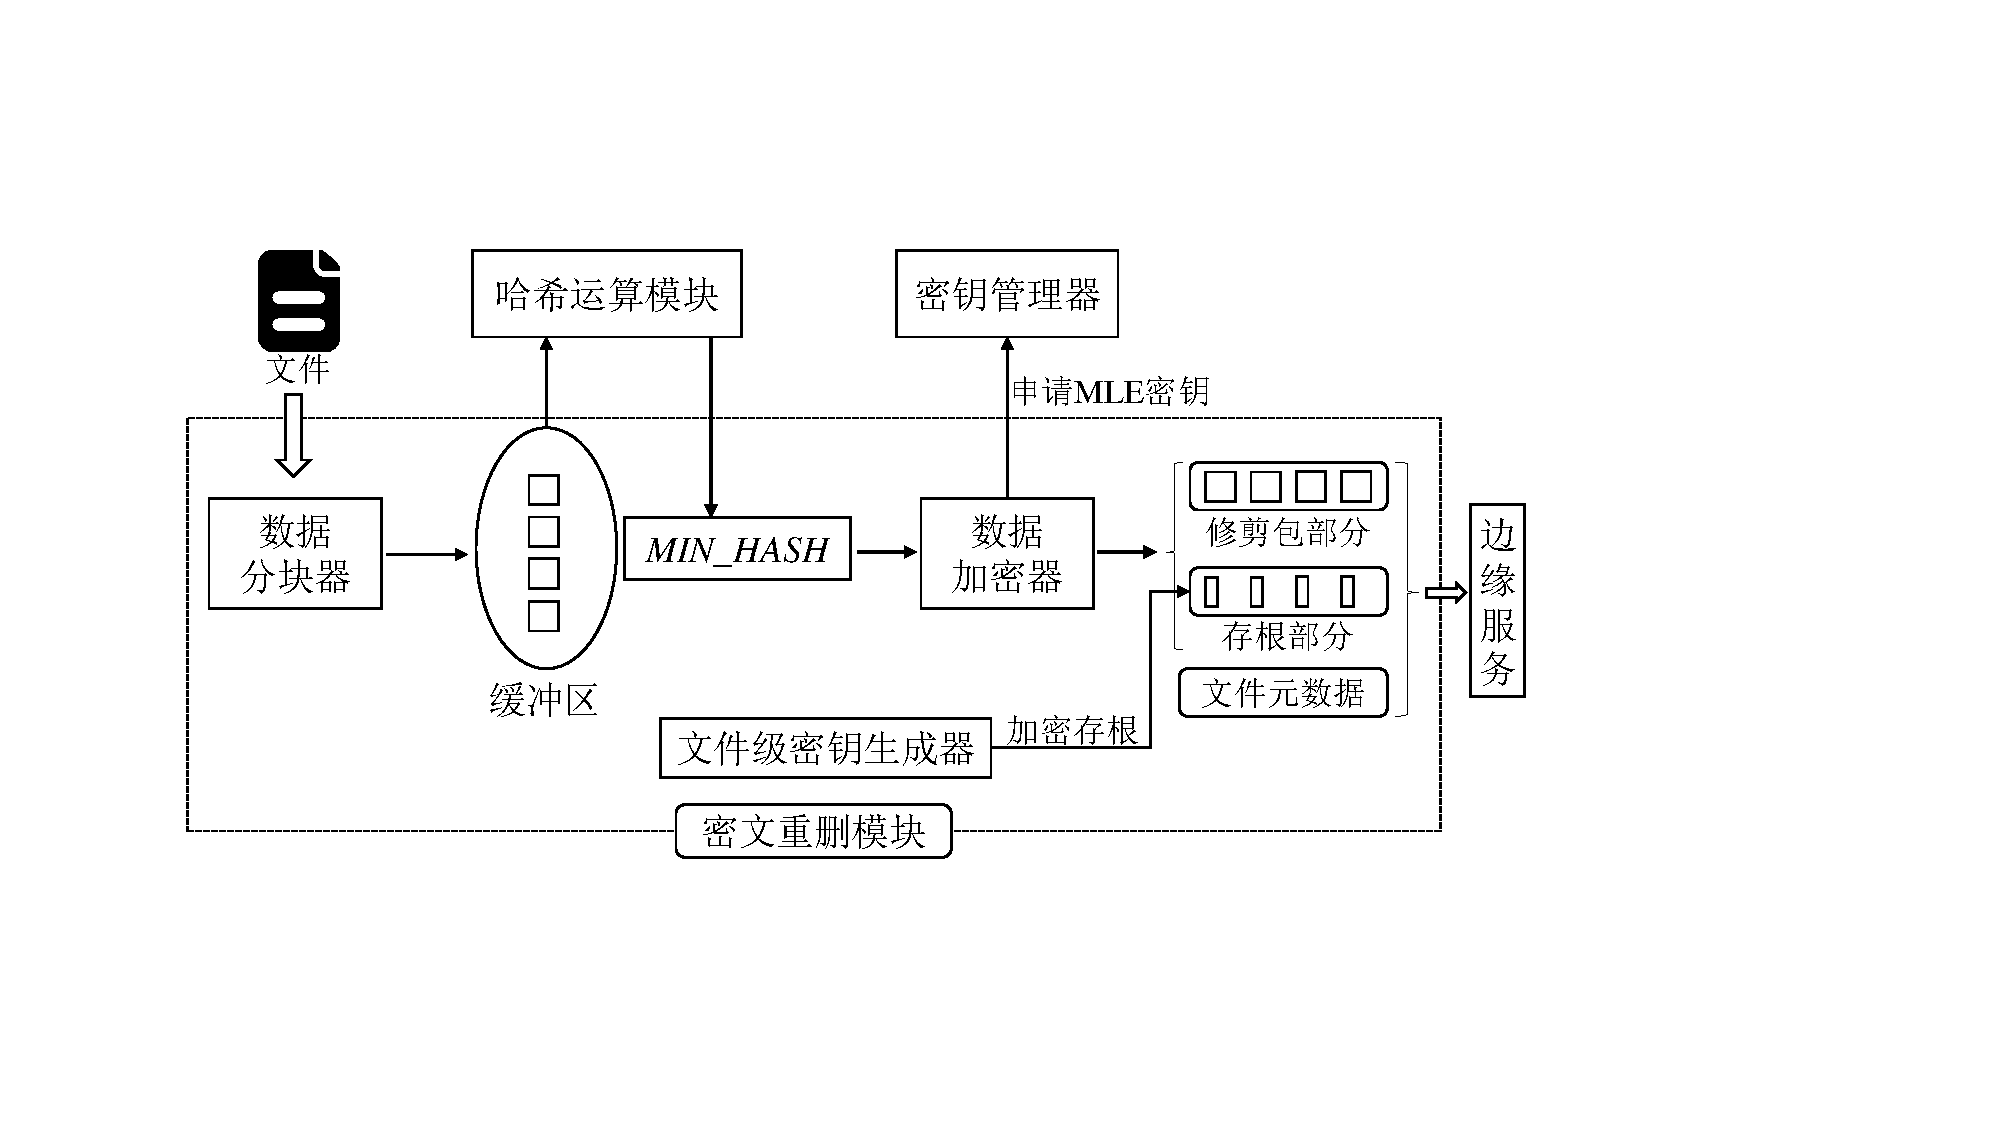
\includegraphics[width = 1.0\linewidth]{pic/密文重删模块.pdf}
    \caption{客户端密文去重模块上传文件关键组件}
    \label{密文去重模块上传文件关键组件}
\end{figure}

上文说提及的文件级密钥,和文件解密以及密钥更新都相关,在此段做详细交代。文件级密钥生成器在初始化时,会选择一个随机的密钥状态值$S_F$(其中$F$代表客户端要上传的某一个文件),利用哈希运算模块计算其哈希值作为文件级密钥$K_F$。由客户端指定一个策略然后用CP-ABE(本论文使用CP-ABE的工具包实现\citing{cpabe})加密密钥状态值$S_F$,该策略信息和被加密的$S_F$也是需要被记录在文件元数据信息表中的,用于其他用户解密获取密钥状态值$S_F$。

上文只关注了文件上传时具体实现,下面将详细介绍文件被下载访问和密钥更新的两种情况。值得注意的是,这两个操作也是在密文去重模块完成的,只不过因为实现并不复杂而没有列出具体组件。

当用户下载一个文件时,客户端会获取$S_F$加密值,并用访问私钥去解密得到密钥状态值明文。然后利用哈希运算模块计算出文件级密钥$K_F$。客户端收到边缘服务器传送的修剪包和存根之后,然后用$K_F$解密所有的存根并按照\ref{CAONT}章节中的加密方案进行反向解密,最后按照文件元数据信息表中的数据块指纹序列(file recipe)形成文件明文。

当用户进行密钥更新时,同样地先获取密钥状态$S_F$明文值,然后使用基于RSA的密钥回归方案\citing{fu2006key}产生新的密钥状态值$S'_F$,由用户指定新策略然后基于CP-ABE加密$S'_F$,将新状态值密文和新策略更新至文件元数据信息表中。系统初始化时,倘若指定积极更新的动态访问控制策略,那么客户端还需要下载文件$F$的所有存根并用密钥状态值$S'_F$生成的文件级密钥重加密,在上传至边缘服务器;倘若指定的是懒惰更新的动态访问控制策略,那么当某客户端在访问时,才会触发重加密操作。根据密钥回归技术,该客户端拥有新密钥状态值,必然能推导出旧密钥状态值,能用旧密钥状态值生成旧文件密钥,再用旧文件密钥解密存根,然后用新文件密钥重加密存根再上传。

最后,简单交代一下客户端上传的文件元数据信息表的详细内容以及安全处理方式。文件元数据信息表是文件被加密存储和解密恢复的重要依据,其包含的重要信息有:文件的标识符(文件的唯一标识)、数据块指纹序列(file recipe)、密钥状态值和密钥状态值被CP-ABE加密所选的策略信息。当然,文件元数据信息表被上传至服务端还会被添加进新的内容,放至服务端实现讲解。本系统采用加密哈希函数模糊化了文件元数据中敏感信息。

(3)密文检索模块

密文检索模块主要支持关键词的安全检索功能,其关联信息的收集主要由关键词切分器和关联信息初始化器两个组件支撑。其中关键词切分器主要用于对明文文件的关键词切分;关联信息初始化器主要用来对切分出来的关键词间,以及关键词与文件之间建立关联,并初始化关联值。下面先简述这两个核心组件在文件上传时收集关键词关联信息的操作,然后再讲述整个模块在密文检索过程中参与的工作。

关键词切分器底层是一个分词器,本系统拟采用一款开源的、高性能中文分词器friso\citing{friso},它使用流行的mmseg算法实现\citing{friso},支持中英或英中混合词的识别。将切分的关键词先利用哈希值运算模块计算出关键词指纹值,将关键词指纹值丢进一个hash表中统计每个关键词出现的次数,供关联信息初始化器获取文件包含的单词的频率,也就是公式\ref{关键词-文件关联度公式}中的$f_{d, KW}$。然后建立关键词-文件的倒排索引(inverted index),本系统采用hash表作为倒排索引的数据结构,用文件的指纹值(文件指纹值是文件的唯一标识符,通过哈希运算模块计算出来的)作为hash表的key值,而hash表的value值是一个列表,列表的每一个元素应该包含关键词的指纹值和关联度初始值(采用\ref{关键词-文件关联度公式}公式计算)两个重要信息。客户端将这些信息发送给边缘服务器,至于边缘服务器用什么样的数据结构高效维护关键词-文件间的关联信息放在\ref{边缘服务器的实现}中详细介绍。

至于关键词与关键词间的关联度信息的提取工作。系统在实现时,指定了参数$len$为0,也就是说,本系统实现时只统计了相邻关键词之间的关联度而忽略了其他距离的关键词关联信息。关联信息初始化器还是以hash表记录每一对关键词的关联度信息。此时,hash表的key应该是某一个关键词指纹值,value应该是一个列表,列表的每一个元素包含两个重要信息:与key代表的关键词相邻的其他关键词指纹值和成对相邻出现的次数。也就是说,相邻关键词出现次数被记录了两次,这样的冗余记录是有必要的:无向图的的相邻结点也是成对出现的,冗余记录两次有助于从任何一个结点找到另一个相邻结点。然后,计算明文文件长度,带入公式\ref{关键词-关键词关联度公式}更新刚刚的hash表的列表中次数值为关联度值。最后,客户端发送hash表至边缘服务。边缘服务器组织和维持关联度信息放在\ref{边缘服务器的实现}章节讲述。

本系统在实现密文检索模块的分词器时,还考虑到一种情况:支持用户不使用系统的分词器而是自己指定文件的关键词。那么这个时候,关联信息初始化器无法完成初始化关联信息操作,需要用户去指定关键词和文件的关联度初始值和关键词间的关联度初始值而不是。为了简单表述这两种初始值等级,本项目统计了若干文件的两种关联度初始化值并选择一个大致的范围:0.1-0.5。所以,为了简化整个系统实现,只给用户五个等级选择:0.1/0.2/0.3/0.4/0.5。初值越小代表着初始关联度越低;初值越大代表着初始关联度越高。

密文检索模块不仅支持收集文件中关联信息,还支持密文关键词的检索。当客户端要检索某一个关键词时,先利用哈希运算模块计算该关键词的指纹值,客户端在检索时带上该指纹值。当边缘服务器返回目标文件的标识符后,密文检索模块会将目标文件的标识符转移给密文去重模块,由密文去重模块完成后续的权限校验和解密恢复明文工作。密文去重模块的后续工作在上述模块中已经详细交代了,此处再简单交代一下:密文去重模块会根据指定文件标识符下载边缘服务器上的文件元数据信息表,根据其中的CP-ABE的策略进行权限验证,合法才能解密其中的密钥状态值并哈希运算得到文件级密钥解密该文件的所有存根部分。

\subsection{边缘服务器}\label{边缘服务器的实现}
边缘服务器核心模块主要是密文去重模块和密文关键词检索模块。其中密文去重模块主要支持文件级的重复辨识和顺序存储文件级密文信息,密文关键词检索模块主要支持整合边缘服务下的所有用户的文件关联信息并维护和更新整个边缘的关联信息。下面分述这两种模块。

(1)密文去重模块

密文去重模块主要由文件元数据索引、修剪包索引、I/O 和磁盘的若干数据分区组成。修剪包索引由磁盘上已经存储的文件的修剪包总指纹和修剪包磁盘起止位置(修剪包是顺序存放的)构成;元数据索引由文件的标识符和文件的元数据信息表存放的磁盘位置信息构成,在内存和磁盘上都有副本,初始化是从磁盘上拷入内存加块系统访问速。值得注意的是,修剪包的总指纹和文件的存根部分位置信息也会被存放在该文件元数据信息表中。I/O主要负责读写磁盘数据,由文件系统提供给用户态的系统调用(read/write)实现。密文去重模块还在磁盘上分出四个区域,修剪包区用来顺序存放文件的修剪包,存根区用来顺序存放文件的存根,元数据区专门用来存放文件元数据信息,索引区用来存放文件的元数据索引表和修剪包索引表,如图\ref{边缘服务器的密文去重模块}。
\begin{figure}[htbp]
    \centering
    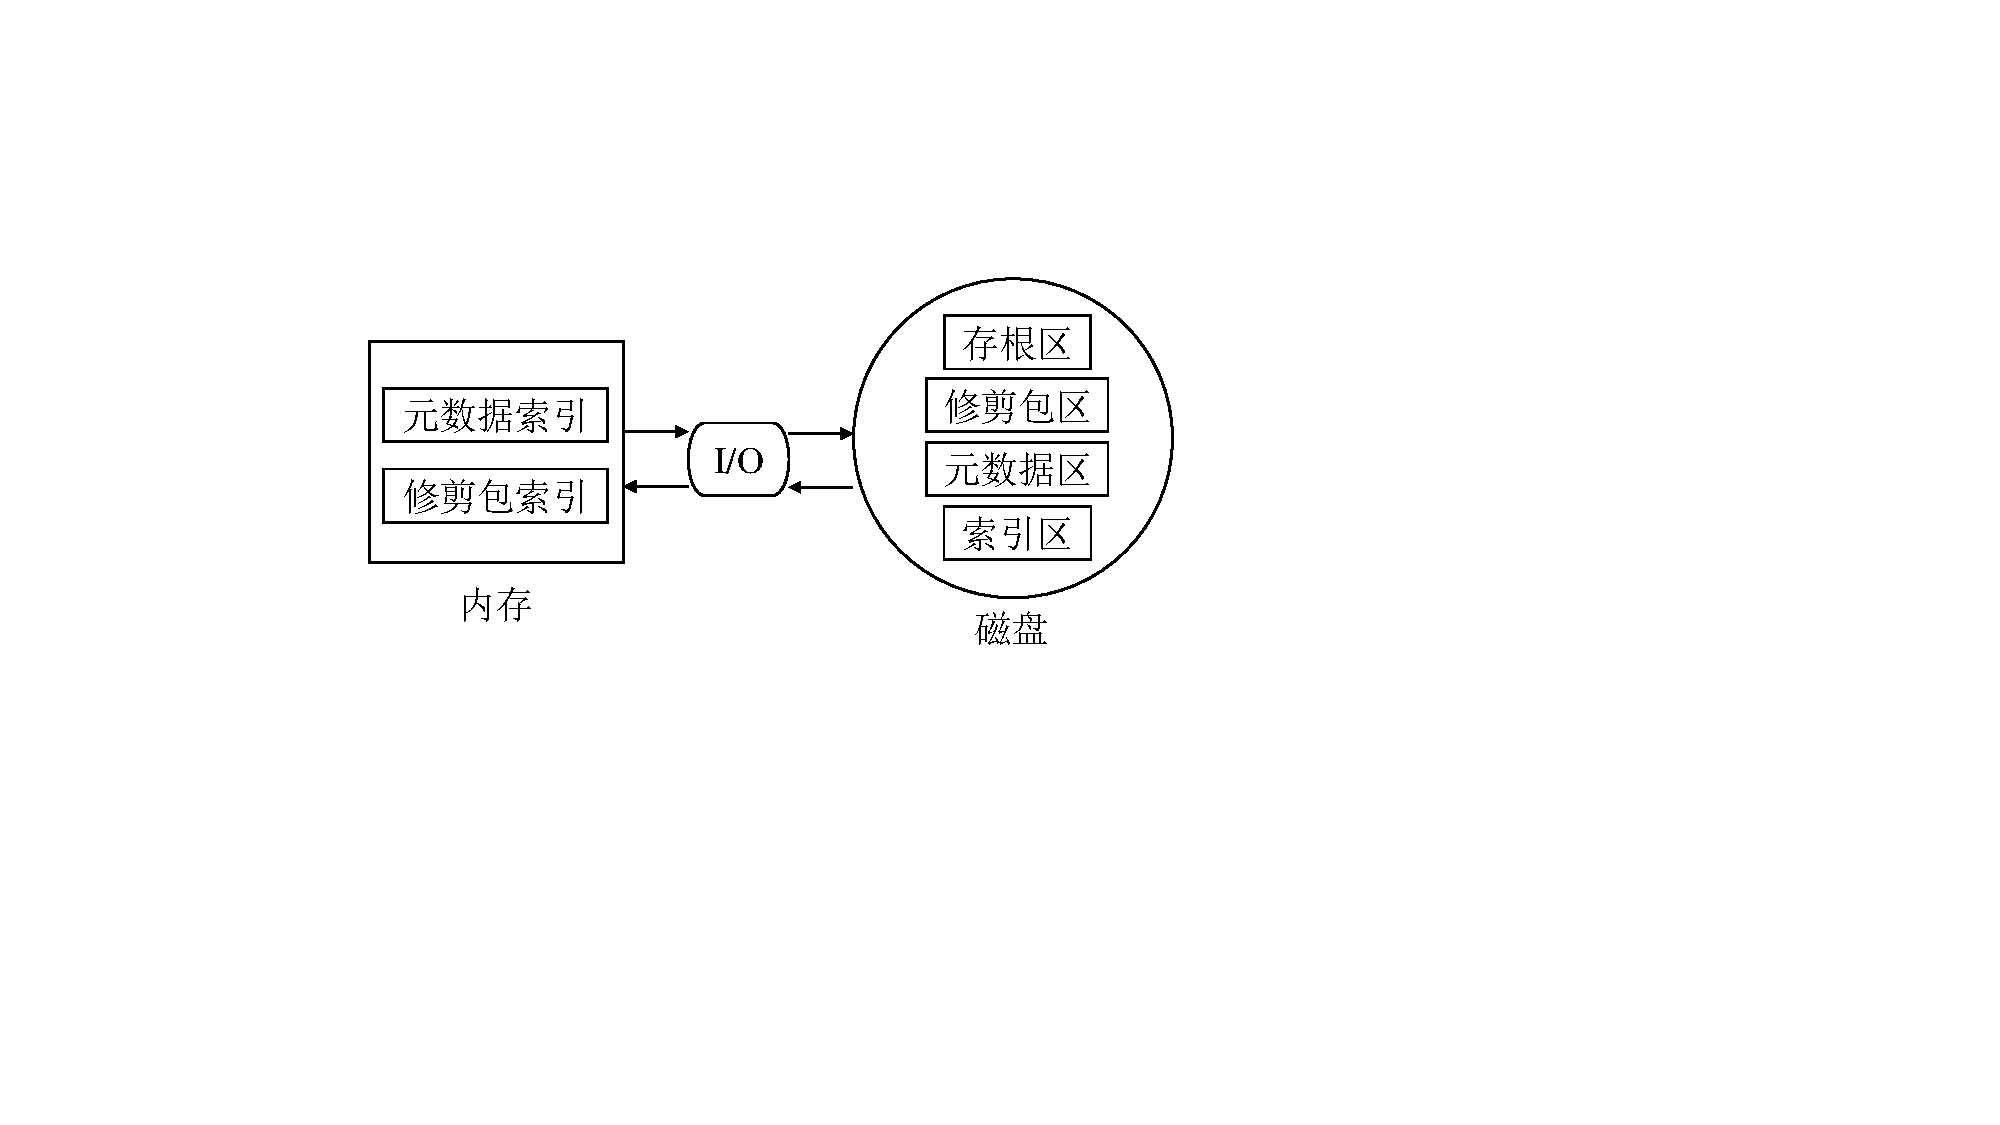
\includegraphics[width = 0.7\linewidth]{pic/边缘服务器的密文重删模块.pdf}
    \caption{边缘服务器的密文去重模块}
    \label{边缘服务器的密文去重模块}
\end{figure}


边缘服务器会将收到的文件的每一个修剪包计算其哈希值然后拼接在一起并对拼接结果计算其哈希值,作为文件的修剪包整体的总指纹并记录在文件元数据信息表中。不得不说明的是再次计算修剪包部分的指纹值的必要性:\ding{172}以此作为该文件修剪包是否在边缘服务器上存储过的标识;\ding{173}文件元数据信息表记录修剪包指纹值有助于访问该文件的用户恢复该文件明文信息。边缘服务器会将总指纹值对照修剪包索引判断文件是否存储过。若没存储过,边缘服务器会调用I/O将修剪包和存根分别顺序写入磁盘的指定区域,并在修剪包索引表和元数据信息表中分别记录下修剪包和存根的磁盘起止位置;若存储过,边缘服务器只会将存根顺序写入磁盘指定区域并在文件元数据信息表中记录下存根的磁盘起止位置。无论文件的修剪包是否被存储过,密文重删模块都要将修建包总指纹记录在文件的元数据信息表中。客户端实现了文件级的去重其实就是实现了文件中修剪包部分的去重,而存根部分可能会被不同的用户用不同的文件级密钥加密所以不支持去重。

当客户端下载文件时,指定文件的标识符后,边缘服务器会检索文件元数据索引找到文件元数据信息表。按照元数据信息表记录的修剪包总指纹查找修剪包索引找到修建包整体;按照元数据信息表中的存根位置信息找到存根部分。将这两个部分和记录在文件元数据信息表中的文件数据块指纹序列信息(file recipe)一并发送给客户端。

上文提及了元数据索引和修建包索引,并没有详细讲解其具体索引结构,我们会在此章节详细开展。现有的研究表明文件级的去重率并不高\citing{chen2015bl},那么对于索引的更新也是写多读少的场景。所以在系统实现时,采用了日志结构合并树(Log-Structured Merge-Tree,LSM-Tree)作为索引结构\citing{o1996log}。LSM-Tree延迟批处理索引变更,然后类似归并排序的方式串联起一个基于内存的组件和若干基于磁盘的组件上面的所有变更信息。相比于传统的B树访问方式大大减少磁盘臂的移动开销。

(2)密文检索模块

密文检索模块主要是收集边缘下各个客户端的关联信息,建立整个边缘的关联并维护更新,涉及两个数据结构:\ding{172}关键词和文件关联的倒排索引;\ding{173}关键词和关键词的无向图。这两个数据结构在\ref{keyword_search}已经详细介绍过,此章节会具体介绍实现部分。

关键词和文件的倒排索引底层采用hash表和大根堆(Max-heap)实现。hash表的key值是关键词的指纹值,hash表的value是大根堆。大根堆的每一个元素包含着两个重要的信息:与它关联文件的指纹值和该文件和key的关键词之后的关联度值,排序是基于关联度值的。在做关联分析和推荐时,边缘服务器返回大根堆的前10项(如果数量足够的话),也就是关联度值最高的10项。然后边缘服务器会向云服务器询问来自其他边缘服务的5项最高关联度的文件,至于云服务收到这样的咨询后续底层实现放在\ref{云服务的实现}中讲解。若客户端选中其中的某一项文件,会在申请文件访问时带上文件的指纹和是否是本边缘服务器下的标识。若来自本边缘服务器,本边缘服务器直接提取文件相关的元数据,存根和修剪包发送给客户端;若来自其他边缘,本边缘带上文件指纹向云服务申请数据,云服务向各边缘服务器申请数据的操作会放在\ref{云服务的实现}中讲解。此外,将选中的文件项会放进一个新的、暂时的大根堆中维持它们的大根堆特性,当某一项被用户选中时,将选中的项中的关联度值加上相应的值:本边缘服务下关联度值增加1,其他边缘服务器下增加0.5。将更新之后的项丢进新的大根堆中,需要维持大根堆特性的时间开销是$O(\log n)$,其中$n$为新大根堆中已有的元素个数。将旧大根堆中还有被选中的数据全部拷贝至新大根堆中,因为这些剩余数据已经拥有了大根堆特性所以不需要进行和父节点大小比较以及重排序。然后将新大根堆设置为hash表的value值,旧的作为暂时空间待下次更新时使用。若没有命中用户想要的文件,边缘服务器会找到次最关联的11项,并向云服务器申请其他边缘服务器上的6个次最关联的的文件,一起返回给客户端。此后,没有命中的话选中的文件项个数会逐步加1,线性扩大推荐的文件范围。

关键词和关键词的无向图底层采用hash表存储,hash的key是关键词指纹值,value是大根堆。大根堆的每一个元素也包含了两个重要的信息:与它关联的关键词及两个关键词之间的关联度,基于关联度排序的。为了存储无向图,也就是说方便无向图的双向查找,同一个边的信息会存放在两个hash表中各一份。例如,在图\ref{关键词-关键词关联度示例图}中$KW_1$和$KW_2$两个关键词的的关联度为$C_{1-2}$,那么在第一个hash表中存在key是$KW_1$且其对应的value是含有\{$KW_2$,$C_{1-2}$\}的大根堆,在第二个hash表中存在key是$KW_2$且其对应的value是含有\{$KW_1$,$C_{1-2}$\}的大根堆。此外,在收集到客户端的各个文件的关键词关联信息时会将这些信息汇总到关键词备案表中。再对不同文件的相同的关键词的关联值做加权处理,比如,在图\ref{关键词-关键词关联度示例图}中$KW_1$和$KW_2$两个关键词的的关联度为$C_{1-2}$,然后这个关联值在不同文件或者客户端都存在,那么边缘服务器会收集加权做为初始值。在做关联分析和推荐时,边缘服务器先找到关键词最相邻的10个关键词(如果足够的话),对得到十个最关联关键词依次执行上段的流程得到的本边缘下100个文件和其他边缘的50个文件,将两部分分别安得分公式\ref{得分公式}计算出结果并置于两个小顶堆$HEAP_1$和$HEAP_2$中,维持小根堆中存放的一定是最关联的若干项,详细算法见\ref{更新小顶堆算法},$HEAP_1$和$HEAP_2$的初始大小分别是10和5。当命中客户端的要求文件时,从关键词备案表中找到该文件所有的相邻关键词并对其间的关联度更新:本边缘增加1,其他边缘的增加0.5,至于快速更新并保持大根堆的结构,还是要借助一个新的、暂时的空大根堆完成;若没有命中,对上述查找相关的变量增加1,也就是说边缘服务器会查找次关联的11个关键词(如果足够的话),并将$HEAP_1$和$HEAP_2$的大小更新为11和6,关键词与文件的范围查找的参数也要增1,比如本边缘下的关联文件个数变成11和其他边缘下的关联文件个数变成6,后面没命中依次线性增大查找参数。


\subsection{云服务器}\label{云服务的实现}
云服务器的底层也是分成两个模块的:密文去重模块和密文检索模块。密文去重模块主要支持数据块级别的去重和共享不同边缘之间的数据;密文检索模块主要支持接受某边缘服务器的密文关键词的询问并转发给各边缘,收取信息返回给边缘服务器。下面细述这两个模块。

(1)密文去重模块

在云服务上主要进行数据块级别的去重,主要需要全局的数据块指纹索引支持。边缘服务器在上传真实数据块之前会先上传文件元数据信息表,云服务器会对照数据块指纹索引标记还没存储过的但在文件元数据信息表中存在的数据块。此后,边缘服务器可根据标记信息上传指纹数据块。云服务器调用系统I/O将数据块随机写入外存,并在数据块指纹索引插入新记录行。在云服务的索引实现中需要考虑到索引过大内存放不下的情况,简单分析一下为什么云服务器需要对索引做出优化而边缘服务器不需要:在\ref{客户端}中提及对文件的指纹提取是用的SHA-256哈希函数,也就是在数据块指纹索引中光指纹占用了32byte,不妨假设磁盘位置信息占4byte\citing{el2012primary},当云服务上有一百万个数据块时,仅指纹占用的空间大约是$100万 * (32byte + 4byte) = 36MB$,当云服务上存储的数据越来越大时,再算上指纹索引中存储着数据块的磁盘位置信息,索引会线性增长下去且占用极大的空间;而边缘服务器上存放的是文件级的索引信息且数据量不会像云服务如此大,内存是绰绰有余的。因此特做出了以下的优化。

优化的核心思想是在内存中存放一个只有2byte大小的压缩索引,它是对数据块指纹的再索引,使用布谷鸟哈希(cuckoo hash)\citing{pagh2004cuckoo}解决哈希函数冲突问题。内存的压缩索引因为将32byte的数据块指纹压缩成2byte,那么会出现内存索引命中但是磁盘的数据块索引中不存在记录的情况(原理和布隆过滤器误判情况类似),同时充当布隆过滤器会筛选掉很大一部分对磁盘的数据块指纹也不存在记录的访问。内存索引对每一个数据存储信息的条目只需要6byte,其中2byte是压缩索引大小(不具有唯一性),4byte是数据块索引条目的磁盘位置信息,那么同样的100万个数据块,只需要占用内存$100万 * 6byte = 6MB$,缩小了6倍,内存空间能够扛得住。此外,为了达到批量I/O的目的,云服务器还实现了写缓冲区(write butter)和预读缓冲区(prefatch cache)。当数据块不存在(新数据块)时,对磁盘中数据块索引的插入操作先写入写缓冲区中,批量插入追加到磁盘的数据块索引日志中;当没有命中内存压缩索引但磁盘的数据块索引却存在时,批量读取10000条数据块索引放于预读取缓冲区供下次访问使用,这充分利用了空间局部性原理。索引的整体架构和流程如下图\ref{云服务器上块级去重的索引架构和查找流程}。
\begin{figure}[htbp]
    \centering
    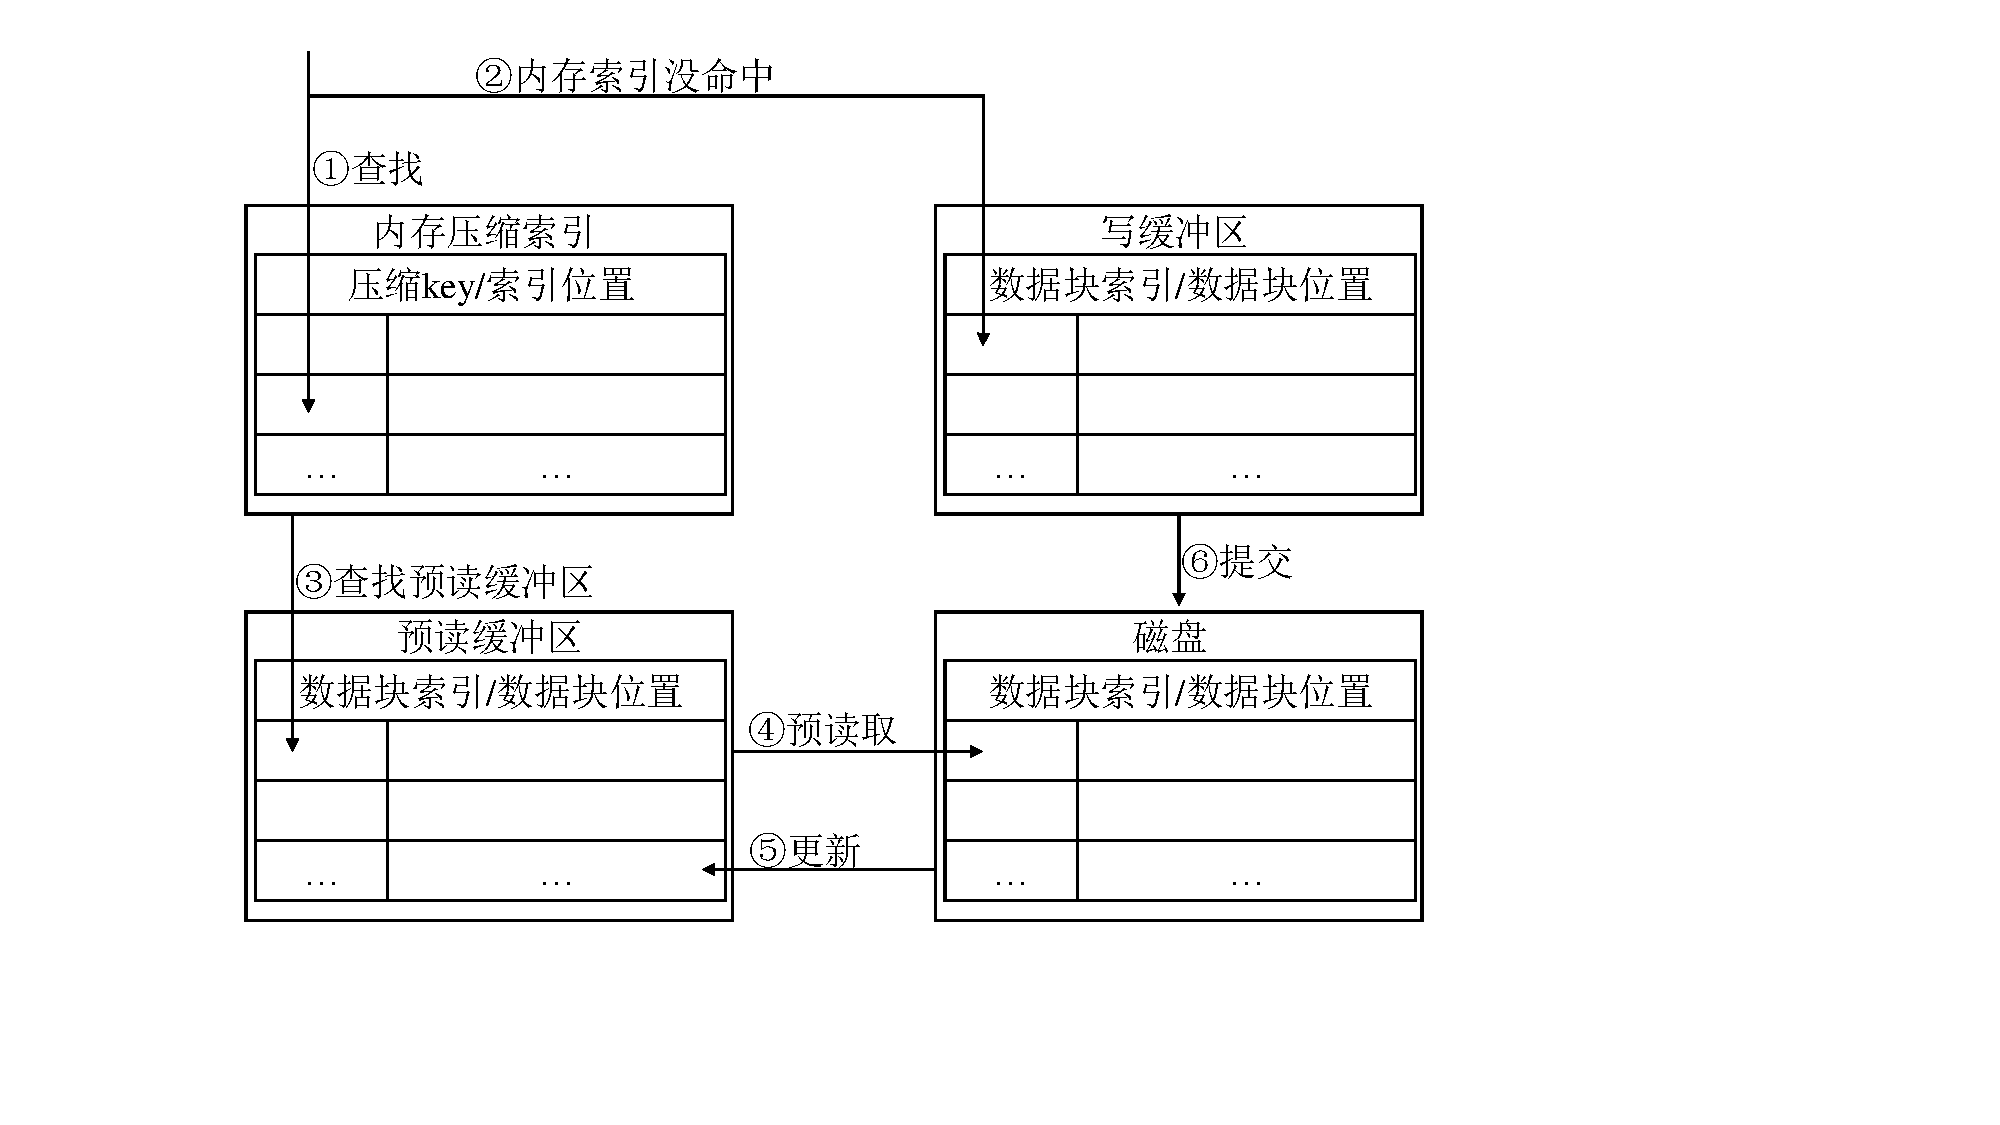
\includegraphics[width = 0.8\linewidth]{pic/云服务器上块级重删的索引架构和查找流程.pdf}
    \caption{云服务器上块级去重的索引架构和查找流程}
    \label{云服务器上块级去重的索引架构和查找流程}
\end{figure}

对数据的块级存储涉及大量的数据块指纹索引的查找操作,对索引的查找和更新可以简化为如下几步:\ding{172}先查找内存的压缩索引,若果不命中说明磁盘中一定没有对应记录存在(原理和布隆过滤器相似),也就是说磁盘一定不存在这个新数据块,那么云服务端需要调用磁盘I/O写入这个数据块,然后记录下磁盘的位置信息并追加到在写缓冲区中,由于磁盘中的数据块索引是基于日志结构的,那么能轻易计算该数据块指纹索引的磁盘位置信息(因为数据块指纹索引条目固定36byte大小,且在内存记录下日志的终点位置即可,当前新条目的起始为磁盘索引日志的终点位置,下一个条目的起始位置为索引日志终点位置加上36byte)。将新数据块索引信息更新至内存压缩索引中,更新索引信息完成。\ding{173}当命中内存压缩索引时,并不能说明磁盘上一定存在对应的条目(反例是布隆过滤器的误判操作),转入下一步。\ding{174}命中内存压缩索引需要去查询预读缓冲区看看真实索引是否存在于读缓冲区中,若不存在还是不能说明磁盘索引中没有对应条目(可能是预读取没命中),转入下一步。\ding{175}根据内存压缩缓冲区查找所有的磁盘索引位置并比对数据的唯一指纹是否是待查找的项,若存在则预读取10000条相邻条目只预读缓冲区并新增一条至内存压缩索引中,其key为压缩索引值,索引位置为刚刚找到的位置信息;若不存在则写入写缓冲区更新内存压缩索引同第\ding{172}。值得注意的是,每次查询真正落到磁盘之前要先对写缓冲区的数据执行提交操作(commit),避免信息已经插入写缓冲区还没落盘的空指针异常问题。此外,系统还设计了背景线程(background thread)每秒对读缓冲进行写提交操作。

云服务器支持不同边缘服务器之间的数据共享主要体现在云服务器收到某边缘服务器对其他边缘服务器的数据访问时,这时云服务器会先向指定边缘服务器索要目标文件的元数据信息表和文件存根部分,然后根据元数据信息提取被存储在磁盘上的数据块一并发送给边缘服务器。换句话说,云服务器只需要将存放在本地的数据块提取出来而不需要向边缘服务再次索要。因为云服务器索引精巧的设计而数据恢复和处理能力要远大于边缘服务器,所以云服务对数据块的随机读写性能相比边缘服务顺序读写的劣势完全可以忽略。此外,还能降低边缘服务到云服务数据块传送产生的网络占用。

(2)密文检索模块

密文检索模块主要为了支持某边缘服务的对其他边缘服务器上文件检索功能。当某边缘服务器$EDGE_1$对云服务器发起其他边缘服务器上文件的检索请求时,云服务收到后会转发给其他的所有边缘服务器,云服务器充当了检索的客户端。当云服务收到边缘服务器所有返回的数据时,它会维持一个大根堆并将所有查询结果置于大根堆中(该大根堆是基于关联度的),然后按照该边缘服务$EDGE_1$查询请求返回相应数量的查询结果,即初次查询返回最关联的5项结果,没命中的话再反回次最关联的6项查询结果,往后依次增大。

\subsection{密钥管理器}
密钥管理器是提供客户端加密数据块过程中所使用的MLE密钥的,使用基于SSL/TLS的授权信道与客户端进行交互。密钥生成的过程完全和DupLESS的OPRF协议\citing{keelveedhi2013dupless}一致。密钥管理器配置了系统范围的公钥/私钥对,该密钥对是基于1024位的RSA生成的。客户端向密钥管理器发送每一个数据块的盲指纹,然后密钥管理器计算盲指纹上的RSA签名,最后客户端对盲签名做签名校验和结果求解并将该结果做哈希运算得到最终的MLE密钥。

\subsection{优化}
以上几个部分分别讲述了系统的各个实体的底层实现,但是没有交代这些实体的技术优化。本小节将在批量操作和并行化操作这两个方面阐述系统实现层面的优化。

(1)批量操作

本系统批量处理小请求以减少网络和I/O开销。如果客户端向密钥管理器发送单独的每个区块MLE密钥生成请求,则会产生大量的往返开销,特别是如果处理许多小尺寸的区块。所以对每个区块的多个密钥生成请求进行批处理,以减少往返开销。此外,在文件上传过程中,客户机在内存缓冲区(当前我们将其大小设置为4MB)中批量处理多个修剪的包,并在缓冲区已满时将批量处理的包发送到服务器。此外,服务器在数据去重后的独特精简包批处理为4MB单元,然后将其存储在存储后端,以减少I/O开销。

(2)并行化操作

本系统利用并行化来提高性能。首先,每个客户端通过多线程并行化加密和解密:它将块分派给多个线程,每个线程对被派分给自己的数据块执行加密和解密。边缘服务器使用多路I/O复用机制的方式响应客户端的各种请求(包括密文检索、上传文件和下载文件等),本系统采用了libevent库\citing{libevent}来实现的边缘服务器和客户端的网络通讯。云服务器只需要和固定数量且为数不多的边缘服务器进行通讯,所以使用了固定的线程和边缘服务器进行通讯(每个边缘服务器对应一个云服务上线程)。

\section{实验实施方案及数据集}
在由多台机器组成的局域网测试台上评估本系统,每台机器都配备了一个24核2.40GHz Intel E5-2620的CPU、20TB的硬盘和32GB内存条,并安装了64位Ubuntu 20.04.1 LTS的操作系统。所有机器都通过1Gb/s交换机连接。

为了性能测试的准确性,本论文给出了10次运行的平均结果。本论文没有将方差结果包括在结果的图中,因为它们在评估中通常很小。本论文中,使用一个合成数据集、两个真实数据集和一个抽样数据集进行评估。

(1)合成数据集

具体来说,自己生成一个2GB的合成数据文件,其中包含全局唯一的块(即,块没有重复的内容)。在每次实验之前,将合成数据加载到内存中,以避免产生任何磁盘I/O开销。合成数据集主要用来测量MLE密钥生成性能、加密性能、上传和下载性能和密钥更新性能。

(2)真实数据集

真实数据集是两个开源的数据集:FSL和VM。其中,FSL数据集由石溪大学(Stony Brook University)的文件系统和存储实验室(File systems and Storage Lab,FSL)收集。原始FSL数据集包含共享文件系统中不同用户的主目录的每日备份。本论文实验专注于2013年的Fslhomes数据集\citing{fsl},该数据集包括2013年1月22日至2013年6月17日的147个每日快照。每个快照代表一个每日备份,由平均8KB块大小的可变大小块的48位指纹集合表示。

VM数据集由虚拟机(Virtual Machine,VM)映像快照组成,是作者的硕士生导师Li等人的研究工作中的数据集\citing{li2015cdstore}。2014年春季,Li等人为参加大学编程课程的学生提供了156个虚拟机。他们在三个月内为每个虚拟机拍摄了26张完整的每日快照。每个快照的大小为10GB,整个数据集包含39.61TB的数据。每个每日快照以4KB固定大小块上的SHA-1指纹表示。删除了已知在VM映像中占主导地位的所有零填充块使得大小减少到28.83TB。
真实数据集主要用来测量存储效能和不涉及分块步骤的上传和下载性能。

(3)抽样数据集

抽样数据集是本人收集的自己以及教研室同门的个人电脑上5G的文本文档数据,这些文本文档数据的拓展名主要是.docx、.doc、.txt、.ppt、.key、和.pages等。这些明文数据主要用来测量提取的关联信息存储空间、建立关联信息的性能和关键词检索性能。

\section{实验结果}
\subsection{MLE密钥生成性能}\label{MLE密钥生成性能}
本小节用合成数据集对客户端和密钥管理器之间的MLE密钥生成性能做出测评。客户端使用基于Rabin指纹的可变大小分块,以指定的平均分块大小创建输入的2GB文件的分块。客户端还将块分组为具有指定平均段大小的可变大小段。客户端计算每个段的最小指纹,并向密钥管理器请求段级MLE密钥。本实验测量MLE密钥生成速度,定义为文件大小(即2GB)与从分块完成到从密钥管理器获得所有MLE密钥的总时间之比,该时间包括计算分段最小hash值时间(若每个分段只有一个数据块,则为0)和申请MLE密钥时间之和。

\ref{密钥生成速度1}展示了段级MLE密钥生成速率随着平均数据块大小变化趋势,其中蓝颜色实线是分段级的密钥生成速度趋势线(固定分段段大小为64KB,例如当平均块大小为2KB时,则32个数据块形成一个分段),红色虚线为数据块级的密钥生成速率趋势线。从块级趋势线看出:块级密钥生成速率基本和平均块大小一样成倍数上涨。此时,更大的数据块意味着更少的数据块数,那么申请MLE的次数也会成倍下降,即密钥生成速度也是成倍上涨。从段级趋势线不难观察到:速度随着平均块大小的增加而增加且增长幅度明显降低(尤其是在块大小为8KB时)。段级密钥生成速度增长是因为分段大小固定说明申请MLE次数固定但是一个分段数据块个数却成倍数减少,客户端需要更少的时间计算分段的代表hash值;增长幅度减小是因为随着段中数据块减少,计算段代表hash值的时间减少幅度逐渐下降而网络带宽(1Gb/s)成为新的瓶颈。

当平均块大小为8KB时,段级密钥生成速度在3.28GB/s左右。当块在2-16KB变动时,MLE密钥生成速率都小于2.5GB/s,其中在平均块大小为8KB时,块级密钥生成速率为1.38GB/s,而分段密钥生成速率大约是其2.6倍。当然,块级密钥生成速率也会随着数据块大小增大而增加,原因在于同一个MLE密钥可以为更大的数据块服务,并且数据块级密钥生成速度不存在饱和线。

\begin{figure}
    \centering
    \begin{subfigure}{0.40\textwidth}
        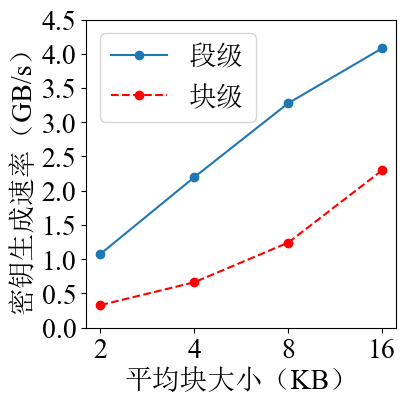
\includegraphics[width=1\linewidth]{pic/gudingfenduan_1.png}
        \centering
        \captionsetup{width=\textwidth}
        \caption{段大小固定为64KB}
        \label{密钥生成速度1}
    \end{subfigure}
    \begin{subfigure}{0.405\textwidth}
        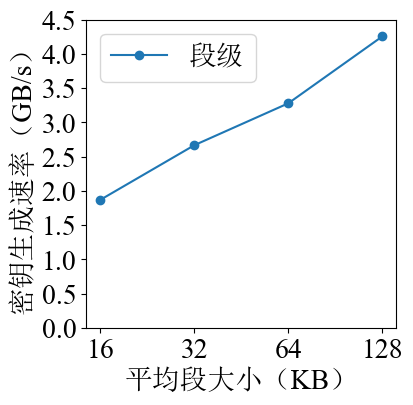
\includegraphics[width=1\linewidth]{pic/gudingfenkuai_1.png}
        \centering
        \captionsetup{width=\textwidth}
        \caption{块大小固定为8KB}
        \label{密钥生成速度2}
    \end{subfigure}\\

    \caption{MLE密钥生成速率变化趋势}
    \label{密钥生成速度}
\end{figure}

当固定数据块大小为8KB时,随着平均分段大小的增大,MLE密钥生成速率增大的趋势如图\ref{密钥生成速度2}所示。速度随着平均段大小而增加,因为较大的段大小意味着要生成的MLE密钥更少。在分段大小在16KB时,密钥生成速率是1.87GB/s;分段大小在128KB时,密钥生成速率是4.26GB/s。分段大小扩大到原来的8倍,而密钥生成速率只扩大到原来的2.27倍密钥生成速度增幅远小于段大小的增加幅度。此处主要的原因有两点:\ding{172}网络带宽只有1Gb/s,严重限制了MLE请求的速度;\ding{173}随着分段中块数量增多,计算最小哈希值作为代表哈希值的计算时间也会变长。总体来说,基于相似性的密钥生成技术使得MLE密钥的计算不再是整个密文去重系统的瓶颈。

\subsection{加密性能}\label{加密性能}
本实验在合成数据集上测量了基本加密方案和增强加密方案的性能。假设客户机已经创建了具有可变大小分块的块,并从密钥管理器获得了MLE密钥。在这里,我们测量的加密速率,定义为文件大小(即2GB)与将所有块加密为修建包和存根的总时间之比。

图\ref{两种加密方案的加速率对比图}显示了基本加密方案和增强加密方案的加密速率与平均块大小的关系(注意,平均段大小对加密速率没有影响)。两种加密方案的吞吐量都随着平均块大小的增加而略微增加,这主要是需要处理的块更少,而增加幅度不大的主要是即使块数变少但是块所含字符变多因而需要更复杂的位运算。基本方案比增强方案更快,因为增强方案引入了额外的加密(见增强加密方案\ref{caont-enhanced})。例如,对于平均块大小8KB,基本方案具有200.20MB/s,比加密速率为125.42MB/s的增强方案中快了60.9\%。尽管两种加密方案之间差距较大,但是两种加密速率在8kb以后都是高于测试台的网络带宽(1Gb/s)的,所以加密不是本系统的主要性能瓶颈。
\begin{figure}[ht]
    \centering
    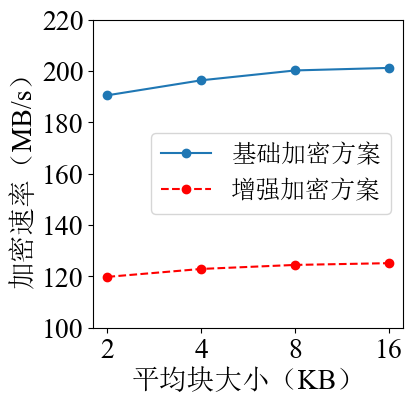
\includegraphics[width = 0.40\linewidth]{pic/jiamisulv.png}
    \caption{两种加密方案的加速率对比图}
    \label{两种加密方案的加速率对比图}
\end{figure}
\subsection{基于合成数据集的上传和下载性能}\label{基于合成数据集的上传和下载性能}
\begin{figure}[h]
    \centering
    \begin{subfigure}{0.40\textwidth}
        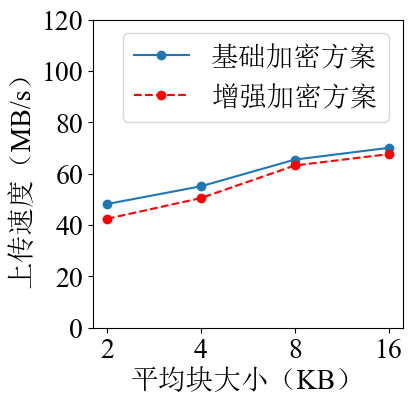
\includegraphics[width=1\linewidth]{pic/upload_chunk_size.png}
        \centering
        \captionsetup{width=\textwidth}
        \caption{上传速度VS块大小}
        \label{上传下载速度1}
    \end{subfigure}
    \begin{subfigure}{0.40\textwidth}
        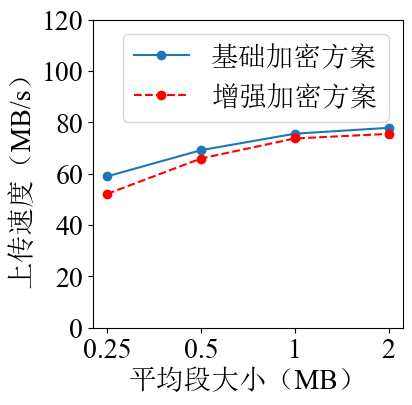
\includegraphics[width=1\linewidth]{pic/upload_segment_size.png}
        \centering
        \captionsetup{width=\textwidth}
        \caption{上传速度VS段大小}
        \label{上传下载速度2}
    \end{subfigure}\\
    \begin{subfigure}{0.40\textwidth}
        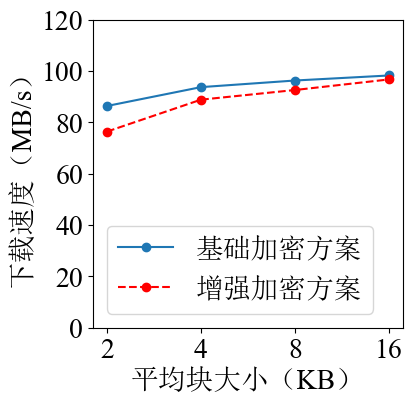
\includegraphics[width=1\linewidth]{pic/download_chunk_size.png}
        \centering
        \captionsetup{width=\textwidth}
        \caption{下载速度}
        \label{上传下载速度3}
    \end{subfigure}
    \begin{subfigure}{0.40\textwidth}
        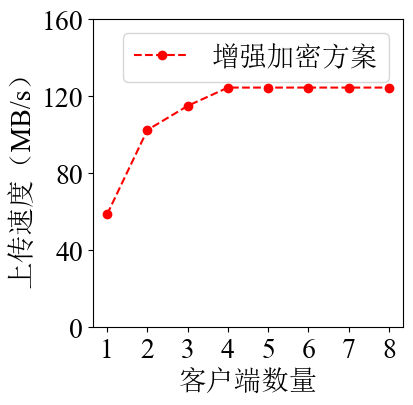
\includegraphics[width=1\linewidth]{pic/upload_client.png}
        \centering
        \captionsetup{width=\textwidth}
        \caption{总上传速度}
        \label{上传下载速度4}
    \end{subfigure}\\
    \caption{上传下载速度}
    \label{上传下载速度}
\end{figure}
% \begin{figure}[h]  
%     \centering  
%     \begin{subfigure}{0.40\textwidth}
%         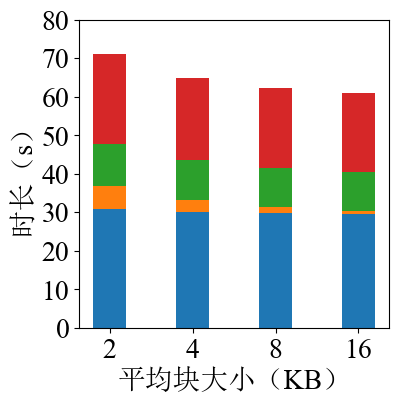
\includegraphics[width=1\linewidth]{pic/basic_encryption_ratio.png}
%         \centering
%         \captionsetup{width=\textwidth}
%         \caption{基础加密方案}
%         \label{上传文件关键步骤时间对比1}
%     \end{subfigure}
%     \begin{subfigure}{0.40\textwidth}
%         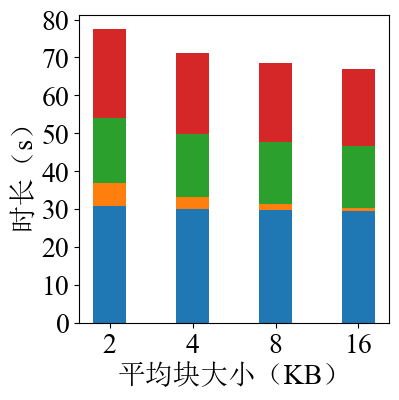
\includegraphics[width=1\linewidth]{pic/enhanced_encryption_ratio.png}
%         \centering
%         \captionsetup{width=\textwidth}
%         \caption{增强加密方案}
%         \label{上传文件关键步骤时间对比2}
%     \end{subfigure}\\
%     \caption{上传文件关键步骤时间对比}
%     \label{上传文件关键步骤时间对比}
% \end{figure}

\begin{figure}[ht]
    \centering
    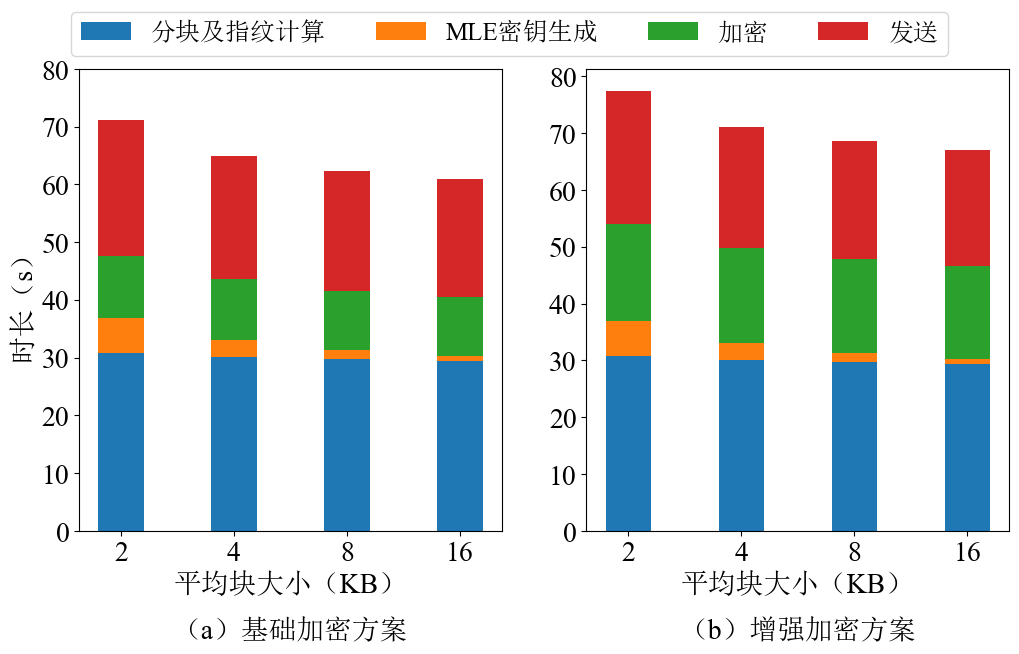
\includegraphics[width = 0.90\linewidth]{pic/basic_enhanced_ratio.png}
    \caption{上传文件关键步骤对比}
    \label{上传文件关键步骤对比}
\end{figure}
本组实验在合成数据集上测量上传和下载性能。对于性能比较,我们还包括了基本加密方案,尽管它在基于相似度的MLE密钥生成中被证明是不安全的。我们首先考虑单个客户的情况。客户端首先上载一个2GB的数据文件,然后下载这个2GB文件。我们将上传速度定义为文件大小与向服务器发送所有文件数据成功的总时间(因为在系统实现时,数据分块、申请MLE密钥、数据加密和数据发送是放在不同的线程中执行的,所以总时间定义为用户输入文件到收到边缘服务器成功接收信号之间的时间差)的比率,将下载速度定义从客户端发出下载请求到恢复所有原始数据的文件大小与总时间(该总时间定义为输入下载请求到接收到客户端恢复成功信号之间的时间差)的比率。在MLE密钥生成性能(见\ref{MLE密钥生成性能})和加密性能\ref{加密性能}两个测量实验中,我们排除了分块的时间,但在本组实验中需要将其纳入时间统计。

图\ref{上传下载速度1}显示了两种加密方案下的上传速度与平均块大小的关系,其中我们将分段平均大小固定为64KB。我们看到,上传速度随着平均块大小的增加而增加。当平均块大小为16KB时,基本方案和增强方案的上传速度分别为70.1MB/s和67.6MB/s。两者离测试台网络带宽(1Gb/s)差距在44\%左右。

图\ref{上传下载速度2}显示了两种加密方案下的上传速度与平均段大小的对比,其中我们将平均块大小固定为8KB。与图\ref{上传下载速度1}类似,上传速度随平均段大小而增长并且两者差距比基于固定分段大小(图\ref{上传下载速度1})还小。例如,当平均段大小为2MB时,基本方案和增强方案的上传速度分别为77.9MB/s和75.5MB/s。两者离测试台网络带宽(1Gb/s)差距在37\%左右。

图\ref{上传下载速度3}显示了两种加密方案下的下载速度与平均块大小的关系(还是固定分段平均大小为64KB)。当平均块大小超过8KB时,两种加密方案的下载速度基本很接近(例如,在块大小为16KB时,基础加密方案的下载速度为98.2MB/s,增强加密方案下载速度为96.7MB/s)。两者比测试台网络带宽(1Gb/s)慢了20\%左右并且下载速率比上传速度要快30\%左右,原因有两点:\ding{172}上传时需要申请MLE密钥;\ding{173}上传数据时需要对数据进行分块操作和数据块指纹计算而恢复数据只需要按照文件元数据表不断拼接数据块。

我们还考虑了多个客户端的情况。将边缘服务器数量设置为1,云服务器的数量设置为1,客户端的数量设置从1个到8个不等,每个客户端运行在不同的进程中(用同一台物理机上的一个进程模拟一个客户端机器)。这里,我们将重点放在增强加密方案下的聚合上载性能上,即每个客户端同时上载一个2GB的唯一数据文件。我们测量总上传速度,定义为文件数据总量(即2GB乘客户端数量)与所有上传完成的总时间之比。图\ref{上传下载速度4}显示了总上传速度与客户端数量的关系,其中我们将平均块大小固定为8KB,平均段大小固定为1MB(128个数据块)。我们看到,速度随着客户端数量的增加而增加,当有8个客户端时,总上传速度达到124.6MB/s,基本接近测试台的网络带宽。

最后,为了说明本轮文的技术点不是整个密文去重系统的瓶颈,特以文件上传为例分析文件上传客户端个阶段的时间比例。文件上传时,需经历四个阶段:数据分块及数据块指纹计算、MLE密钥申请、数据块加密和数据发送。由于在系统实现时,采用了并行化优化手段,这四个步骤放在四个线程中协同完成,所以在各自线程中单独统计每个步骤的时长(也就是完成2G合成数据集上传的各自步骤时间)。分块方式或分段方式对除MLE密钥申请以外的其他三个步骤时长不具备实质干扰,所以我们以分块方式为例,分别考察基础加密方案和增加加密方案下的各个步骤时长,并将其绘制在堆积柱状图中。图\ref{上传文件关键步骤对比}中左图和右图分别展示了基础加密方案和增强加密方案关键步骤在各自线程中的运行时长。不难发现,数据分块和指纹计算时长大于其他各步骤。例如,在增强加密方案中当数据块大小为8KB时,数据分块及指纹计算时间为29.7s,而MLE密钥生成、数据加密和数据发送时间分别为1.6s、16.5s和20.8s。作为下游的三个操作都快于上游的数据分块和指纹计算操作,而又受限于上游。即使采用了并行化的操作,分块及指纹计算也成了整个系统的瓶颈所在,当然这也是其他密文去重系统仍没有解决的问题。所以,分块及指纹计算成了文件上传速度低于测试台带宽(1Gb/s)40\%左右的主要原因。

\subsection{密钥更新性能}

我们在合成数据集上测量了主动更新和懒惰更新方案中的密钥更新性能。本系统的重加密操作需要使用原始策略进行CP-ABE解密,并使用新策略进行另一次CP-ABE加密。本系统将每个策略视为具有连接所有授权用户标识符的或门的访问树,这意味着CP-ABE解密时间是恒定的,而其加密时间随着新策略中授权用户的数量而增长。因此,我们重点评估重加密操作中三个参数的影响:\ding{172}用户总数,即原始策略中的授权用户数;\ding{173}撤销比率,将被撤销并从访问树中删除的用户数量的百分比;以及\ding{174}文件大小,即重新加密文件的大小。我们测量重加密的延迟,定义为执行所有重加密步骤的总时间,包括:下载和解密密钥状态、导出新的密钥状态、加密和上传密钥状态以及重加密存根部分(仅对主动更新而言)。

图\ref{密钥更新性能1}显示了重加密延迟与用户总数的关系,同时我们将重加密的文件大小固定为2GB,撤销率固定为20\%。两种撤销方案的重密钥延迟都随着用户总数的增加而增加,这主要是因为CP-ABE加密开销随着访问树的增大而增加。然而,两种更新方案中的重加密延迟都在4秒内。具体来说,懒惰更新比主动更新快大约0.4秒,因为它将重新加密过程推迟到下一次文件更新。

图\ref{密钥更新性能2}显示了重加密延迟与撤销率的关系,同时我们将重加密的文件大小固定为2GB,用户总数固定为500。随着撤销率的提高,新策略的授权用户减少,从而缩短了撤销时间。当撤销率为50\%时,懒惰更新和主动更新方案的重加密延迟分别为2.90s和2.49s。

图\ref{密钥更新性能3}显示了重加密延迟与重加密文件大小的关系,同时我们将用户总数固定为500,撤销率固定为20\%。重加密文件大小对懒惰撤销没有影响,其中重加密延迟保持在3.11s左右。对于主动更新,随着文件大小的增加,它将花费更多的时间来传输和重新加密存根文件。因此,例如,对于8GB文件,重加密延迟增加到4.55s。然而,如果我们将主动更新的重加密延迟与在网络中传输整个文件的时间(例如,1Gb/s网络中至少65秒)进行比较,那么重加密延迟是无关紧要的。因此,本系统中的重加密操作总体上是轻量级的。

\begin{figure}[h]
    \centering
    \begin{subfigure}{0.40\textwidth}
        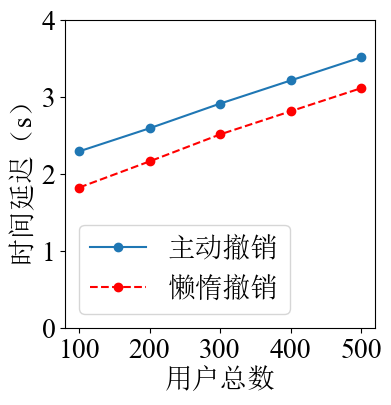
\includegraphics[width=1\linewidth]{pic/user_num.png}
        \centering
        \captionsetup{width=\textwidth}
        \caption{时间延迟VS用户量}
        \label{密钥更新性能1}
    \end{subfigure}
    \begin{subfigure}{0.40\textwidth}
        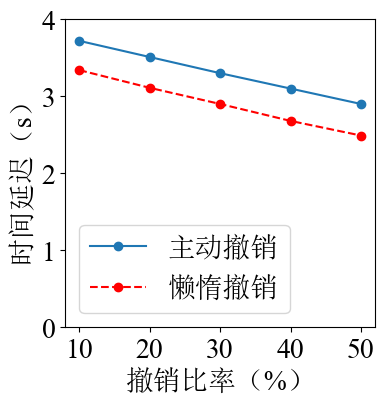
\includegraphics[width=1\linewidth]{pic/revocation_ratio.png}
        \centering
        \captionsetup{width=\textwidth}
        \caption{时间延迟VS撤销率}
        \label{密钥更新性能2}
    \end{subfigure}\\
    \begin{subfigure}{0.40\textwidth}
        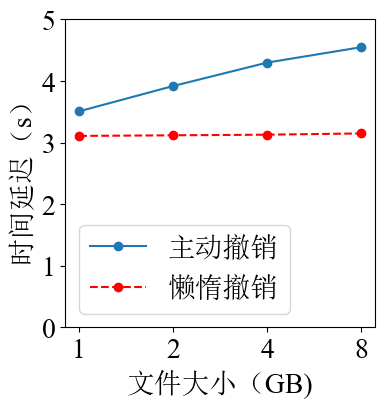
\includegraphics[width=1\linewidth]{pic/file_size.png}
        \centering
        \captionsetup{width=\textwidth}
        \caption{时间延迟VS文件大小}
        \label{密钥更新性能3}
    \end{subfigure}
    \caption{密钥更新性能}
    \label{密钥更新性能}
\end{figure}

\subsection{数据去重的存储开销}\label{存储开销实验}
本组实验是在两个真实数据集上测量存储开销。我们将两个真实数据集尽量均等地分成2MB为大小的片段中,以分段方式申请MLE密钥。
\begin{figure}
    \centering
    \begin{subfigure}{0.40\textwidth}
        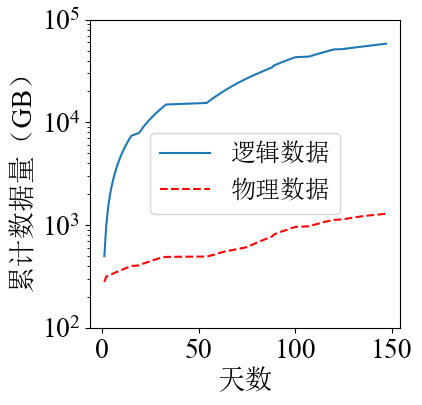
\includegraphics[width=1\linewidth]{pic/fsl_overhead.png}
        \centering
        \captionsetup{width=\textwidth}
        \caption{去重前后(FSL)}
        \label{存储开销1}
    \end{subfigure}
    \begin{subfigure}{0.40\textwidth}
        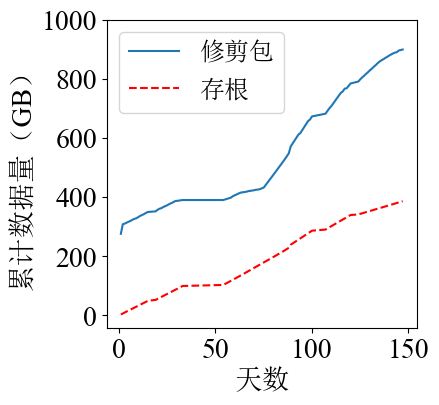
\includegraphics[width=1\linewidth]{pic/fsl_phy_stub.png}
        \centering
        \captionsetup{width=\textwidth}
        \caption{修建包和存根(FSL)}
        \label{存储开销2}
    \end{subfigure}\\
    \begin{subfigure}{0.40\textwidth}
        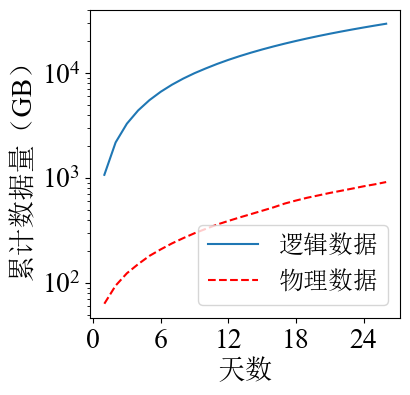
\includegraphics[width=1\linewidth]{pic/ms_overhead.png}
        \centering
        \captionsetup{width=\textwidth}
        \caption{去重前后(VM)}
        \label{存储开销3}
    \end{subfigure}
    \begin{subfigure}{0.40\textwidth}
        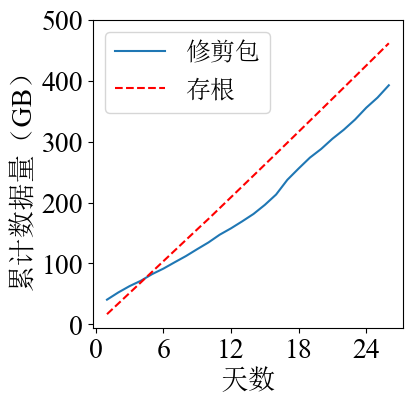
\includegraphics[width=1\linewidth]{pic/ms_phy_stub.png}
        \centering
        \captionsetup{width=\textwidth}
        \caption{修建包和存根(VM)}
        \label{存储开销4}
    \end{subfigure}\\
    \begin{subfigure}{0.40\textwidth}
        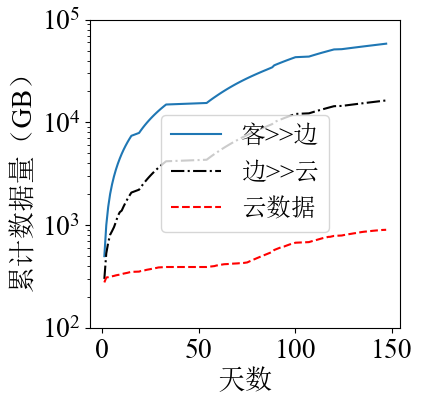
\includegraphics[width=1\linewidth]{pic/fsl_edge_cloud.png}
        \centering
        \captionsetup{width=\textwidth}
        \caption{云/边存储的数据量(FSL)}
        \label{存储开销5}
    \end{subfigure}
    \caption{存储开销}
    \label{存储开销}
\end{figure}

首先测量本系统的存储开销。即使本系统只能对一部分数据块(即修建包)进行数据去重,它仍然通过数据去重来保持存储效率。我们定义了两种类型的数据:\ding{172}逻辑数据,即任何加密或数据去重之前的原始数据;\ding{173}存根,所述加密存根文件被存储;\ding{174}修剪包,所述经修剪的包在数据去重之后被存储。我们聚合所有用户的数据,并测量每个数据类型的总大小。

图\ref{存储开销1}显示了存储所有用户的FSL每日备份的天数内的累积数据大小。每个FSL每日备份包含所有用户的290-680GB逻辑数据,但本系统在数据去重后实际存储的修剪包数据和存根数据平均每天仅为8.75GB。147天后,总共有58435.4GB的逻辑数据,而本系统在数据去重后仅生成1285.6GB的物理数据(即修剪包和存根的总和)。总节约97.8\%。这表明,仍然通过数据去重保持了较高的存储效率。

图\ref{存储开销2}比较了数据去重后修剪包和存根的累积大小。三类数据的大小随着时间的推移而增加。147天后,有899.2GB的修建包,还有386.4GB的存根数据,其中存根部分增幅相对较大。值得注意的是,由于存根数据由可更新的文件密钥加密,因此无法对其进行数据去重。然而,根据图\ref{存储开销1},数据去重有效地减少了总体存储空间。

VM数据集的去重前后变化趋势见图\ref{存储开销3}。图\ref{存储开销3}比较了逻辑数据的大小与物理数据(包括修剪包和存根)的大小。经过26次每日备份,我们总共有29526.8GB的逻辑数据。数据去重将物理数据空间减少到945.2GB。存储节省率为96.8\%。图\ref{存储开销4}显示了一个细节:我们观察到存根数据的大小随每日备份的数量呈线性增长。原因是存根数据大小取决于逻辑块的数量,但每个VM每日备份都有相似数量的逻辑块(不包括零填充块)。26天后,本系统存储483.8GB修建包,461.4GB存根数据。这表明,在VM数据集上任然通过数据去重保持较高的存储效率。

我们进一步比较了基于相似性的方法与原始基于块的方法的存储开销,该方法以块的粒度执行数据去重(FSL为8KB,VM为4KB)。表\ref{使用不同去重方法的物理数据和存根大小对比}显示了修建包和存根大小,以及与原始逻辑数据大小相比节省的存储空间。基于相似性的方法相较于基于块的方法减小了的MLE密钥生成开销,同时导致修剪包的大小增加35.3\%和45.8\%(其中FSL数据集逻辑数据总量58435.4GB,VM数据集逻辑数据总量29526.8GB)。请注意,数据去重技术不会改变逻辑块的总数,因此对于每个数据集而言两种方法的存根数据大小相同。尽管如此,基于相似性的方法仍然为两个数据集实现了与基于块的方法几乎相同的存储节省。本系统专注于通过数据去重技术来保持逻辑数据的高存储节约,但我们观察到,随着存储更多备份,存根数据在物理存储中占主导地位(或者更一般地,对于具有高数据去重节约的工作负载)。为了减轻存根数据的存储开销,一种选择是增加块大小;事实上,已经表明,通过减少元数据开销,更大的块大小可以实现更高的有效存储节省\citing{sun2016long}。

\begin{table}[htbp]
    \begin{center}
        \caption{使用不同去重方法的修剪包和存根大小对比}
        \label{使用不同去重方法的物理数据和存根大小对比}
        \begin{tabular}{|c|c|c|c|}
            \hline
            \multicolumn{2}{|c|}{\textbf{数据}}     & \textbf{基于数据块} & \textbf{基于数据片段}                   \\
            \hline\hline
            \multirow{2}{*}{FSL}                    & 修剪包              & 665.4GB                       & 899.2GB \\

            \cline{2-4}
                                                    & 存根                & \multicolumn{2}{|c|}{386.4GB}           \\
            % \cline{2-4}
            % & 关联信息 &  \multicolumn{2}{|c|}{20.2GB}\\
            \hline
            \multicolumn{2}{|c|}{\textbf{存储节约}} & 98.2\%              & 97.8\%                                  \\
            \hline\hline
            \multirow{2}{*}{VM}                     & 修剪包              & 395.0GB                       & 453.9GB \\
            \cline{2-4} %表示画一条2列-4列的横线
                                                    & 存根                & \multicolumn{2}{|c|}{461.3GB}           \\
            % \cline{2-4}
            % & 关联信息 &  \multicolumn{2}{|c|}{8.5GB}\\
            \hline
            \multicolumn{2}{|c|}{\textbf{存储节约}} & 97.1\%              & 96.9\%                                  \\
            \hline
        \end{tabular}
    \end{center}
\end{table}

最后,我们测量客户端发送给边缘服务器、边缘服务器发送给云服务器以及云服务器上存放的数据量。我们选用一台物理机作为边缘服务器,一台物理机作为云服务器,统计三个阶段的数据量,见图\ref{存储开销5}。在第147天时,从客户端发送给边缘服务器的数据量是58435.4GB,而边缘服务器发送给云服务器的数量为1632.0GB,云服务器上经过数据去重后的数据量是899.2GB(实际上就是修剪包部分数据量),不难发现边缘服务器的文件级去重使得转递给云服务器的数据量下降了72\%。边缘服务器作为云服务器的中间缓存层,对大数据流进行了预去重(即文件级去重)的效果显著。

\subsection{基于trace驱动的上传和下载性能}
\begin{figure}[H]
    \centering
    \begin{subfigure}{0.92\textwidth}
        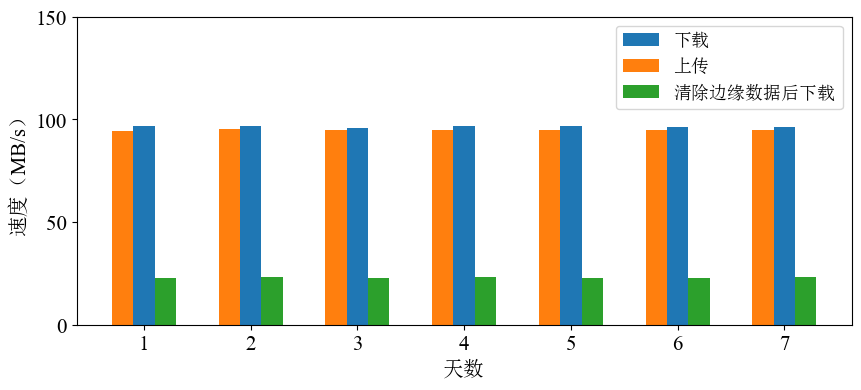
\includegraphics[width=1\linewidth]{pic/real_fsl_upload_download.png}
        \centering
        \captionsetup{width=\textwidth}
        \caption{FSL}
        \label{基于trace驱动的上传和下载性能1}
    \end{subfigure}
    \begin{subfigure}{0.60\textwidth}
        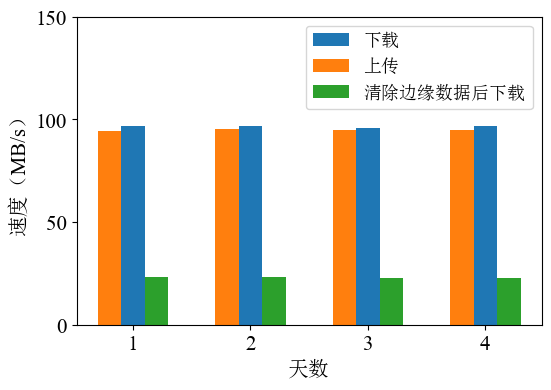
\includegraphics[width=1\linewidth]
        {pic/real_vm_upload_download.png}
        \centering
        \captionsetup{width=\textwidth}
        \caption{VM}
        \label{基于trace驱动的上传和下载性能2}
    \end{subfigure}
    \caption{基于trace驱动的上传和下载性能}
    \label{基于trace驱动的上传和下载性能}
\end{figure}


我们使用两个真实世界数据集(FSL和VM)来评估单个客户端的上传和下载速度,而不是实验\ref{基于合成数据集的上传和下载性能}中的合成数据集的上传和下载性能。由于FSL和VM数据集都只包括块指纹和块大小,我们通过重复将其指纹写入备用块来重建块,直到达到指定的块大小;这确保了相同指纹返回相同的块。重构的块被客户端当做数据分块器执行的分块结果。因此,我们在这个实验中不包括分块时间。此外,存储开销实验显示边缘存储开销较大,所以本组实验中测试下载性能时,我们还做了对比:将边缘服务器上的修剪包数据清除掉,每次下载时边缘服务器向云存储索要修剪包的下载性能测试实验。

客户端(代表所有用户)上载所有每日备份。由于数据集很大,我们只运行部分数据集以减少评估时间。具体而言,对于FSL数据集,我们为九个用户选择了7次连续的每日备份,在数据去重之前,总计3471.7GB的数据;对于VM数据集,我们为所有用户选择了4次每日备份,在数据去重之前总共备份4407.3GB的数据。我们使用与实验\ref{基于合成数据集的上传和下载性能}中相同的设置,并使用增强的加密方案。

图\ref{基于trace驱动的上传和下载性能}显示了几天内的上传和下载速度。从这幅图不难出来两点:\ding{172}没有分块操作的上传下载性能很接近网络带宽(基本在95MB/s以上);\ding{173}清空边缘服务器上的修剪包后再下载的速度远低于从边缘获取修剪包的下载速度,约是其20\%左右。所以,在边缘服务上存储较大冗余的数据能获取很大的下载性能收益。此外,在多机边缘的现实场景中,并行下载的速度理论上成倍上涨。


\subsection{关联信息存储开销与关键词检索性能}
\begin{figure}[htbp]
    \centering
    \begin{subfigure}{0.40\textwidth}
        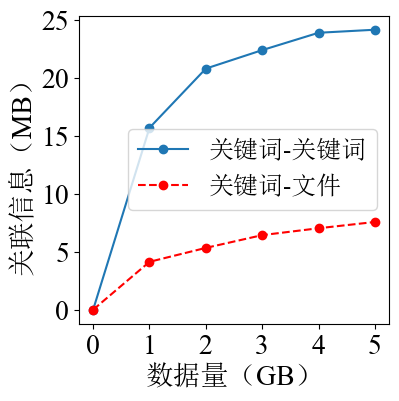
\includegraphics[width=1\linewidth]{pic/keyword_storage.png}
        \centering
        \captionsetup{width=\textwidth}
        \caption{关联信息存储开销}
        \label{关联信息存储开销}
    \end{subfigure}\\
    \begin{subfigure}{0.40\textwidth}
        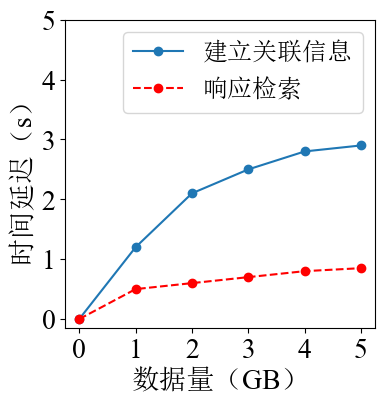
\includegraphics[width=1\linewidth]{pic/keyword_search.png}
        \centering
        \captionsetup{width=\textwidth}
        \caption{两种时间占用对比}
        \label{关键词检索性能1}
    \end{subfigure}
    \begin{subfigure}{0.425\textwidth}
        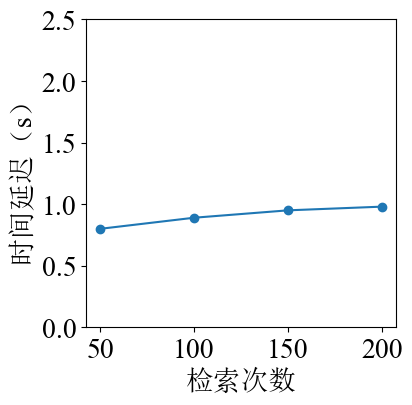
\includegraphics[width=1\linewidth]{pic/time_search_num.png}
        \centering
        \captionsetup{width=\textwidth}
        \caption{关联信息更新}
        \label{关键词检索性能2}
    \end{subfigure}
    \caption{关联信息存储开销与关键词检索性能}
    \label{关联信息存储开销与关键词检索性能}
\end{figure}
为了支持密文关键词检索功能,本系统在边缘服务器上存储了关联信息。那么在本组实验中,我们用抽样数据集对存储关联信息的存储开销和检索性能两方面做了测量。

首先对关联信息存储开销做出测量,图\ref{关联信息存储开销}展示了关键词间的关联信息和关键词与文件的关联信息的存储开销。不难发现,关键词间的关联信息占空间比关键词与文件间的关联信息更大,例如在数据量达到5GB时关键词间的关联信息是24.1MB而关键词与文件间的关联信息是7.6MB。此外,两种关联信息总和占逻辑数据0.62\%,也就是说,对于数据去重系统而言,这点存储开销是微乎其微的。其次,两种关联信息涨到幅度都是先快后慢,这是因为逻辑数据逐步增大,新关键词(unique keyword)个数和新逻辑文件(unique file)个数不会线性增加而是不断重复出现已有的关键词和文件,即关键词和文件的频率增加,那么收集关联信息就演变成更新频率值,存储关联信息的数据结构也不会线性增大。

然后,将两种时间延迟随着数据量变化的曲线绘制在下图\ref{关键词检索性能1}中,不难发现:响应检索的时间占比很小,例如,在数据量达到5GB时,建立关联信息的时间为2.9s而响应检索的时间为0.85s,响应检索的时间占比22.6\%左右。还有一点值得注意的是:随着数据量的不断增大,建立关联的信息和响应检索的时间增幅会逐步减小。原因和关联信息存储开销相似。

此外,以上文200GB已经提取好关联信息并存储在边缘服务上为目标,分别检索任意10个关键词50次、100次、150次和200次并将其响应检索的时间取平均值,绘制成折线图如下\ref{关键词检索性能2}。不难发现,检索次数增加而更新关联信息对响应检索时间延迟的影响是微乎其微的(图中的折线只有轻微涨动)。


\section{本章小结}
本章主要分为两个部分,第一部分详细地介绍了整个系统各个组成的底层实现和优化,其中至关重要的是客户端的实现。作为和用户的交互接口,边缘服务器直接为客户端提供服务,云服务器的实现核心在于对庞大的数据块索引进行压缩索引方式的优化加快了索引访问速度;第二部分主要是整个实验环节:先交代了实验的实施方案,然后从各个方面展示实验的结果以及本系统的性能优势。

\chapter{全文总结与展望}\label{展望}
\section{全文总结}
在过去的十几年期间,数据去重技术飞速发展,其中包括对数据块分块融合机器学习算法的研究、对文件级和数据块级多粒度的去重研究和对整个密文去重系统架构的研究,还有相关研究涉及密文去重系统里面的数据恢复、密文系统中关键词检索以及多服务器的分布式密文去重系统。本文算得上鲜有的涉及“云边协同”架构下的兼容关键词检索的密文去重技术的工作。

本文的主要贡献有三个:

(1)本文较为全面完整的介绍了整个密文去重系统,不仅包括了核心思想,还包括了底层各组件的实现。其中对CAONT技术转化,很好地升级数据加密和去重的核心功能点,与此同时,还能为提供主动和懒惰更新的动态访问控制提供坚实的基础。经过实验验证,整体上数据的存储开销可节约95\%以上,其中边缘服务器存储开销节约70\%左右而云服务器上的存储开销节约高达97\%。在保障尽可能节约存储开销的前提下,数据的上传和下载性能、数据的加密和解密效率等各方面较为优秀。

(2)本论文首次提出了一种全新的、适用于动态更新关联信息以备启发后来检索行为的主动分析和推荐的密文检索技术。该技术不仅能让服务器在线学习用户的检索行为,还能保证极好的用户检索体验,此外关联信息占用空间极小。实验数据表明:关联信息占用物理空间仅占去重之后的所有物理数据的2\%,而经过200次随机的检索,对用户检索响应时间稳定在0.8s左右。

(3)本文的密文去重技术和密文检索技术不是空中建楼阁,而是对“云边协同”架构具有很好的适配性:边缘服务器作为客户端直接服务的提供者,与客户端进行信息交换;云服务器作为各个边缘共享数据的中间者,不仅和各个边缘服务器建立唯一的通信信道,还充当密文检索请求的转发者和共享修建包的数据提供者。

\section{后续展望}
本论文的系统看似完美,实则还有很多不足,未来的工作可在以下几个方面做进一步研究:

(1)服务器高可用性设计。系统设计时只考虑了云服务器中心化设计,而落地时还需要考虑到高可用性的设计:需要将云服务器搭建成主从模式,当主节点宕机后,立马从从节点中选出可用的新主来保证云服务器的各个功能的高可用。边缘服务器也是同理。

(2)服务器存储的可扩展性。本文系统的设计没有考虑到存储容量达到单台机器上限的情况,而工业生成的情况相当复杂,且数据量十分庞大。将机器扩展成集群模式需要考虑到数据的均匀存储和容灾备份的设计。

(3)数据恢复问题。数据去重系统都要面临一个棘手的数据恢复(data restore)问题:用户总是期望系统能在极短的时间内从容器中提取出数据并按照元数据恢复成文件原始内容。因此,研究者在设计系统时总是将热点数据多备份存储以便更快地并行化提取。

\thesisacknowledgement

% 硕士研究生生活是既漫长又短暂的。漫长在于三年的学习生活期间仿佛做了很多有成就的事情:从化学跨考的计算机专业,从懵懂无知的计算机小白到对计算机专业有了初步的系统了解,从对专业知识一问三不知的状态到研究生各科成绩较为优秀并获得过专业一等奖学金的小成就,从刚进入电子科技大学内心的紧张和对未来的迷茫到快毕业时找到了工作的踏实;短暂在于三年的研究生生涯如白云苍狗一晃而逝,依稀记得刚入学的不安与惶恐。但无论如何,研究生三年该在此画上圆满的句号,感谢我身边的每一个人,正是他们的出现才使得我的生活充分乐趣和满足。

% 首先,感谢我的导师李经纬老师。李老师是一位做研究严谨认真,做学问孜孜不倦的人。李老师在我懈怠时勉励我前进,在我学习、做研究过程中给我带来极大的帮助和支持,包容我的缺陷和不足,支持我的一切选择。此外,有幸在研二的时候参加了李老师的婚礼并做了李老师的伴郎,见证了李老师的爱情,终生难忘。作为李老师最拉胯的、最不听话的学生,在毕业之际衷心地祝愿李老师身体健康,工作顺利。

% 其次,感谢我身边的同学们。我的室友卢辉同学机智幽默,乐观豁达。在做研究上总是能高瞻远瞩,乐此不疲;在生活方面,总是能以幽默的语言面对、诙谐的行为处理各种生活的坎坷。从卢辉同学身上,我总能学到一切难以从书本上获取的思维方式,这是他经过学习和揣摩后的独到的知识见解。我的同门唐兴鹏同学沉稳内敛,给我的学习和研究带来了很多帮助和支持;我的两位师兄任彦璟和黄苏豫,知识渊博、涉猎广泛,黄苏豫师兄温柔善良,给了我很多帮助,总能从他身上学会了很多东西。

%  最后,感谢我的父母。我想如果天使真能降落人间的话,那一定是我们每个人的父母。他们总是把生命中最宝贵的东西给我们,让我们有砥砺前行的基石、有披荆斩棘的智慧、有乘风破浪的勇气。

\thesisbibliography[large]{reference} % 参考文献

% \thesisappendix
% \chapter{xxxx} % 直接填写附录内容,写法与正文一致

% 攻读学位期间成果(本科不添加),例如:
\begin{thesistheaccomplish}
    % \section{学术论文}
    % \bibitem{SGXDedup} \textbf{Ren, Yanjing} and Li, Jingwei and Yang, Zuoru and Lee, Patrick PC and Zhang, Xiaosong. Accelerating Encrypted Deduplication via SGX[C]. Proc.of USENIX ATC, 2021, 957-971. \textbf{CCF-A}
    % \section{发明专利}
    % \bibitem{CN111338572B} 李经纬, 杨祚儒, \textbf{任彦璟}, 李柏晴, 张小松. 一种可调节加密重复数据删除方法:CN111338572B[P]. 2021-09-14.
    % \section{参与项目}
    \bibitem{2022YFB4501200} 云边融合的安全存储系统,国家重点研发计划青年科学家项目: 2022YFB4501200. 2023.03 - 2026.02(参与)
    \bibitem{2022YFB3103503} 多媒体大数据安全查询与高效验证技术,国家重点研发计划课题: 2022YFB3103503. 2022.12 - 2025.11(参与)
    \bibitem{2021YFG0167} 面向加密重复数据删除的元数据安全管理及应用, 四川省重点研发计划项目: 2021YFG0167. 2020.04 - 2023.03(参与)

    % \section{奖学金}
    \bibitem{三等奖学金} 电子科技大学学业三等奖学金. 2022.12
    \bibitem{一等奖学金} 电子科技大学学业一等奖学金. 2021.12
    \bibitem{二等奖学金} 电子科技大学入学二等奖学金. 2020.09
\end{thesistheaccomplish}

% 以下为本科同学专用,插入文献翻译
%\thesistranslationoriginal
%\section{Tahoe-LAFS: The Least-Authority File System}
% \insertPDFPage{} % 用于插入单页PDF文件,例如原始文献(该操作会导致页码被取消,请谨慎使用)

%\thesistranslationchinese
%\section{Tahoe-LAFS:最小权限文件系统}

\end{document}